\documentclass[a4paper,12pt]{article}
\usepackage[latin1]{inputenc} %entrada usando ISO-Latin1
\usepackage{listings}
\usepackage{color}
\usepackage{a4wide}
\usepackage{graphicx}
\usepackage{subfig}
\usepackage{wrapfig}
\usepackage{hyperref}
\usepackage{amsmath}
\usepackage{tikz}
\usetikzlibrary{shapes, arrows}
\usepackage{appendix}

\usepackage{bm, amssymb, pifont, pgfplots, multirow, float, soul, color, verbatim, indentfirst}

\newcommand{\be}{\begin{equation}}
\newcommand{\ee}{\end{equation}}

\lstset{
   breaklines=true,
   basicstyle=\ttfamily}
% \usepackage{draftwatermark}
\usepackage[figurewithin=section,tablewithin=section]{caption}
%\usepackage{subfigure}
\setcounter{secnumdepth}{4}

\pagestyle{headings}

\title{\textbf{LCLS-II System simulations:\\Back-end}}
\author{LBNL LLRF Team}

\date{\today}

\begin{document}
\numberwithin{equation}{section} 
\maketitle
\setcounter{tocdepth}{2}
\tableofcontents

\newpage

\section{Overview}

\begin{figure}
\centering
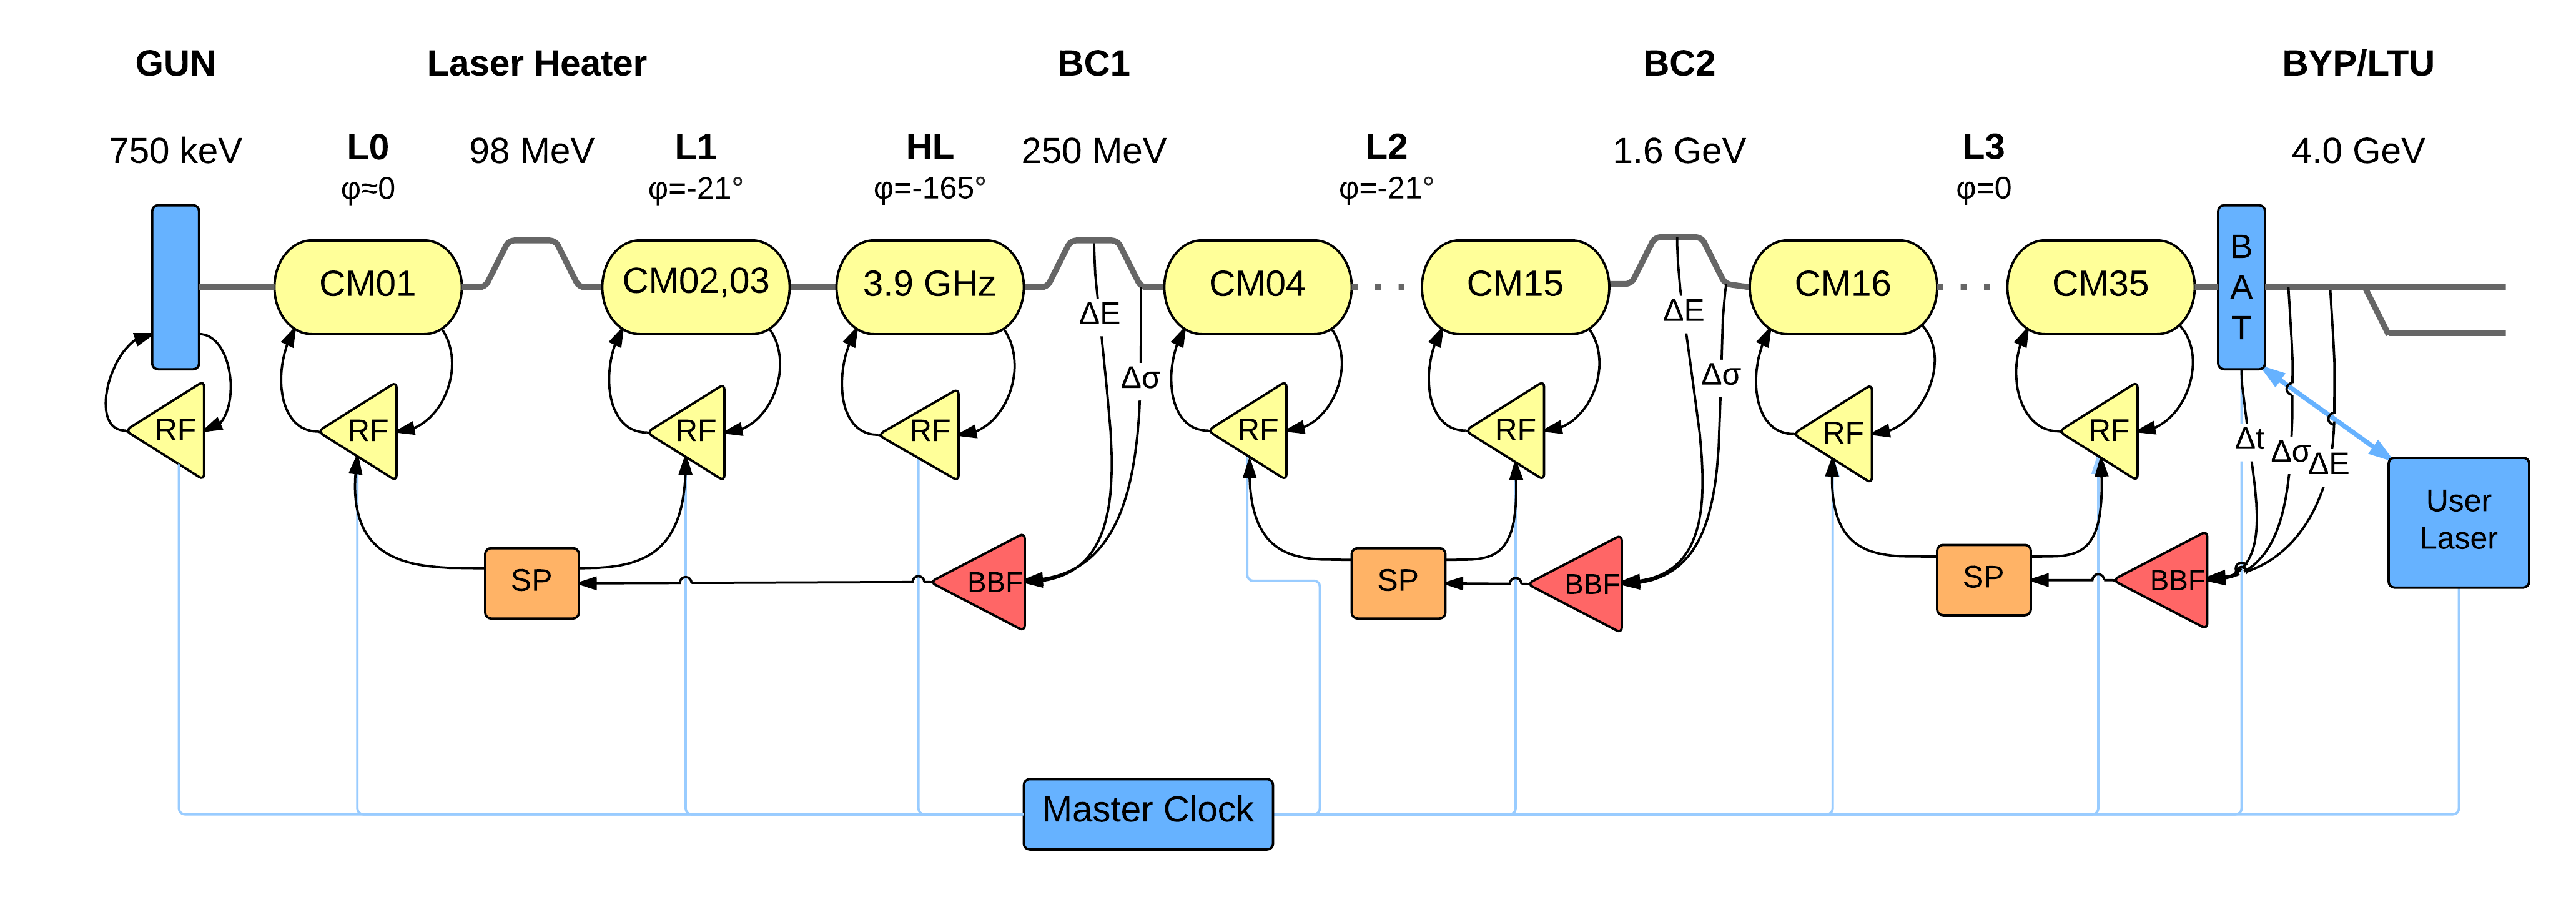
\includegraphics[scale=0.11]{../figures/LCLS-II_feedback_layout.png}
\caption{LCLS-II feedback layout.}
\label{fig:lclsII-feedback_layout}
\end{figure}

During the design, commissioning and operations of a Linac-driven FEL it is useful to have modeling capabilities to abstract and analyze some of the complex problems involved in LLRF and beam-based feedback in the comfortable environment of computer simulations. The simulation framework presented here is a dramatic improvement of a previous version written in Octave/Matlab~\cite{ref:model-paper}, where extensively tested LLRF models are integrated with a longitudinal phase space tracking simulator~\cite{ref:litrack} along with the interaction between the two via beam-based feedback using a computationally efficient simulation engine. 

The models include beam instrumentation, considerations on loop delays for in both the LLRF and beam-based feedback loops, as well as the ability to inject noise (both correlated and uncorrelated) at different points of the machine including a full characterization of the electron gun performance parameters. The Linac is divided into generic compounds composed of an accelerating section followed by a bunch compressor (where the bunch compressor can be enabled/disabled) and beam performance parameters are measured at any stage of the machine for characterization and/or for use to apply beam-based feedback. Time-series data is computed at a configurable simulation step size and results can be visualized in both time and frequency domain, including transfer functions between any noise source and beam performance parameters.

Figure~\ref{fig:lclsII-feedback_layout} shows a high-level representation of the LCLS-II layout, as configured at the time of this writing. The model described here represents each component of the machine in a way that configuration parameters can be adapted as the machine layout and configuration evolves (during the design or in future upgrades), where the contribution of each noise source (correlated or uncorrelated) to the machine performance budget can be quantified, including the ability to represent the effectiveness of different feedback loops to reduce noise contributions under different configurations. 

\section{Model hierarchy}

\begin{figure}
\centering
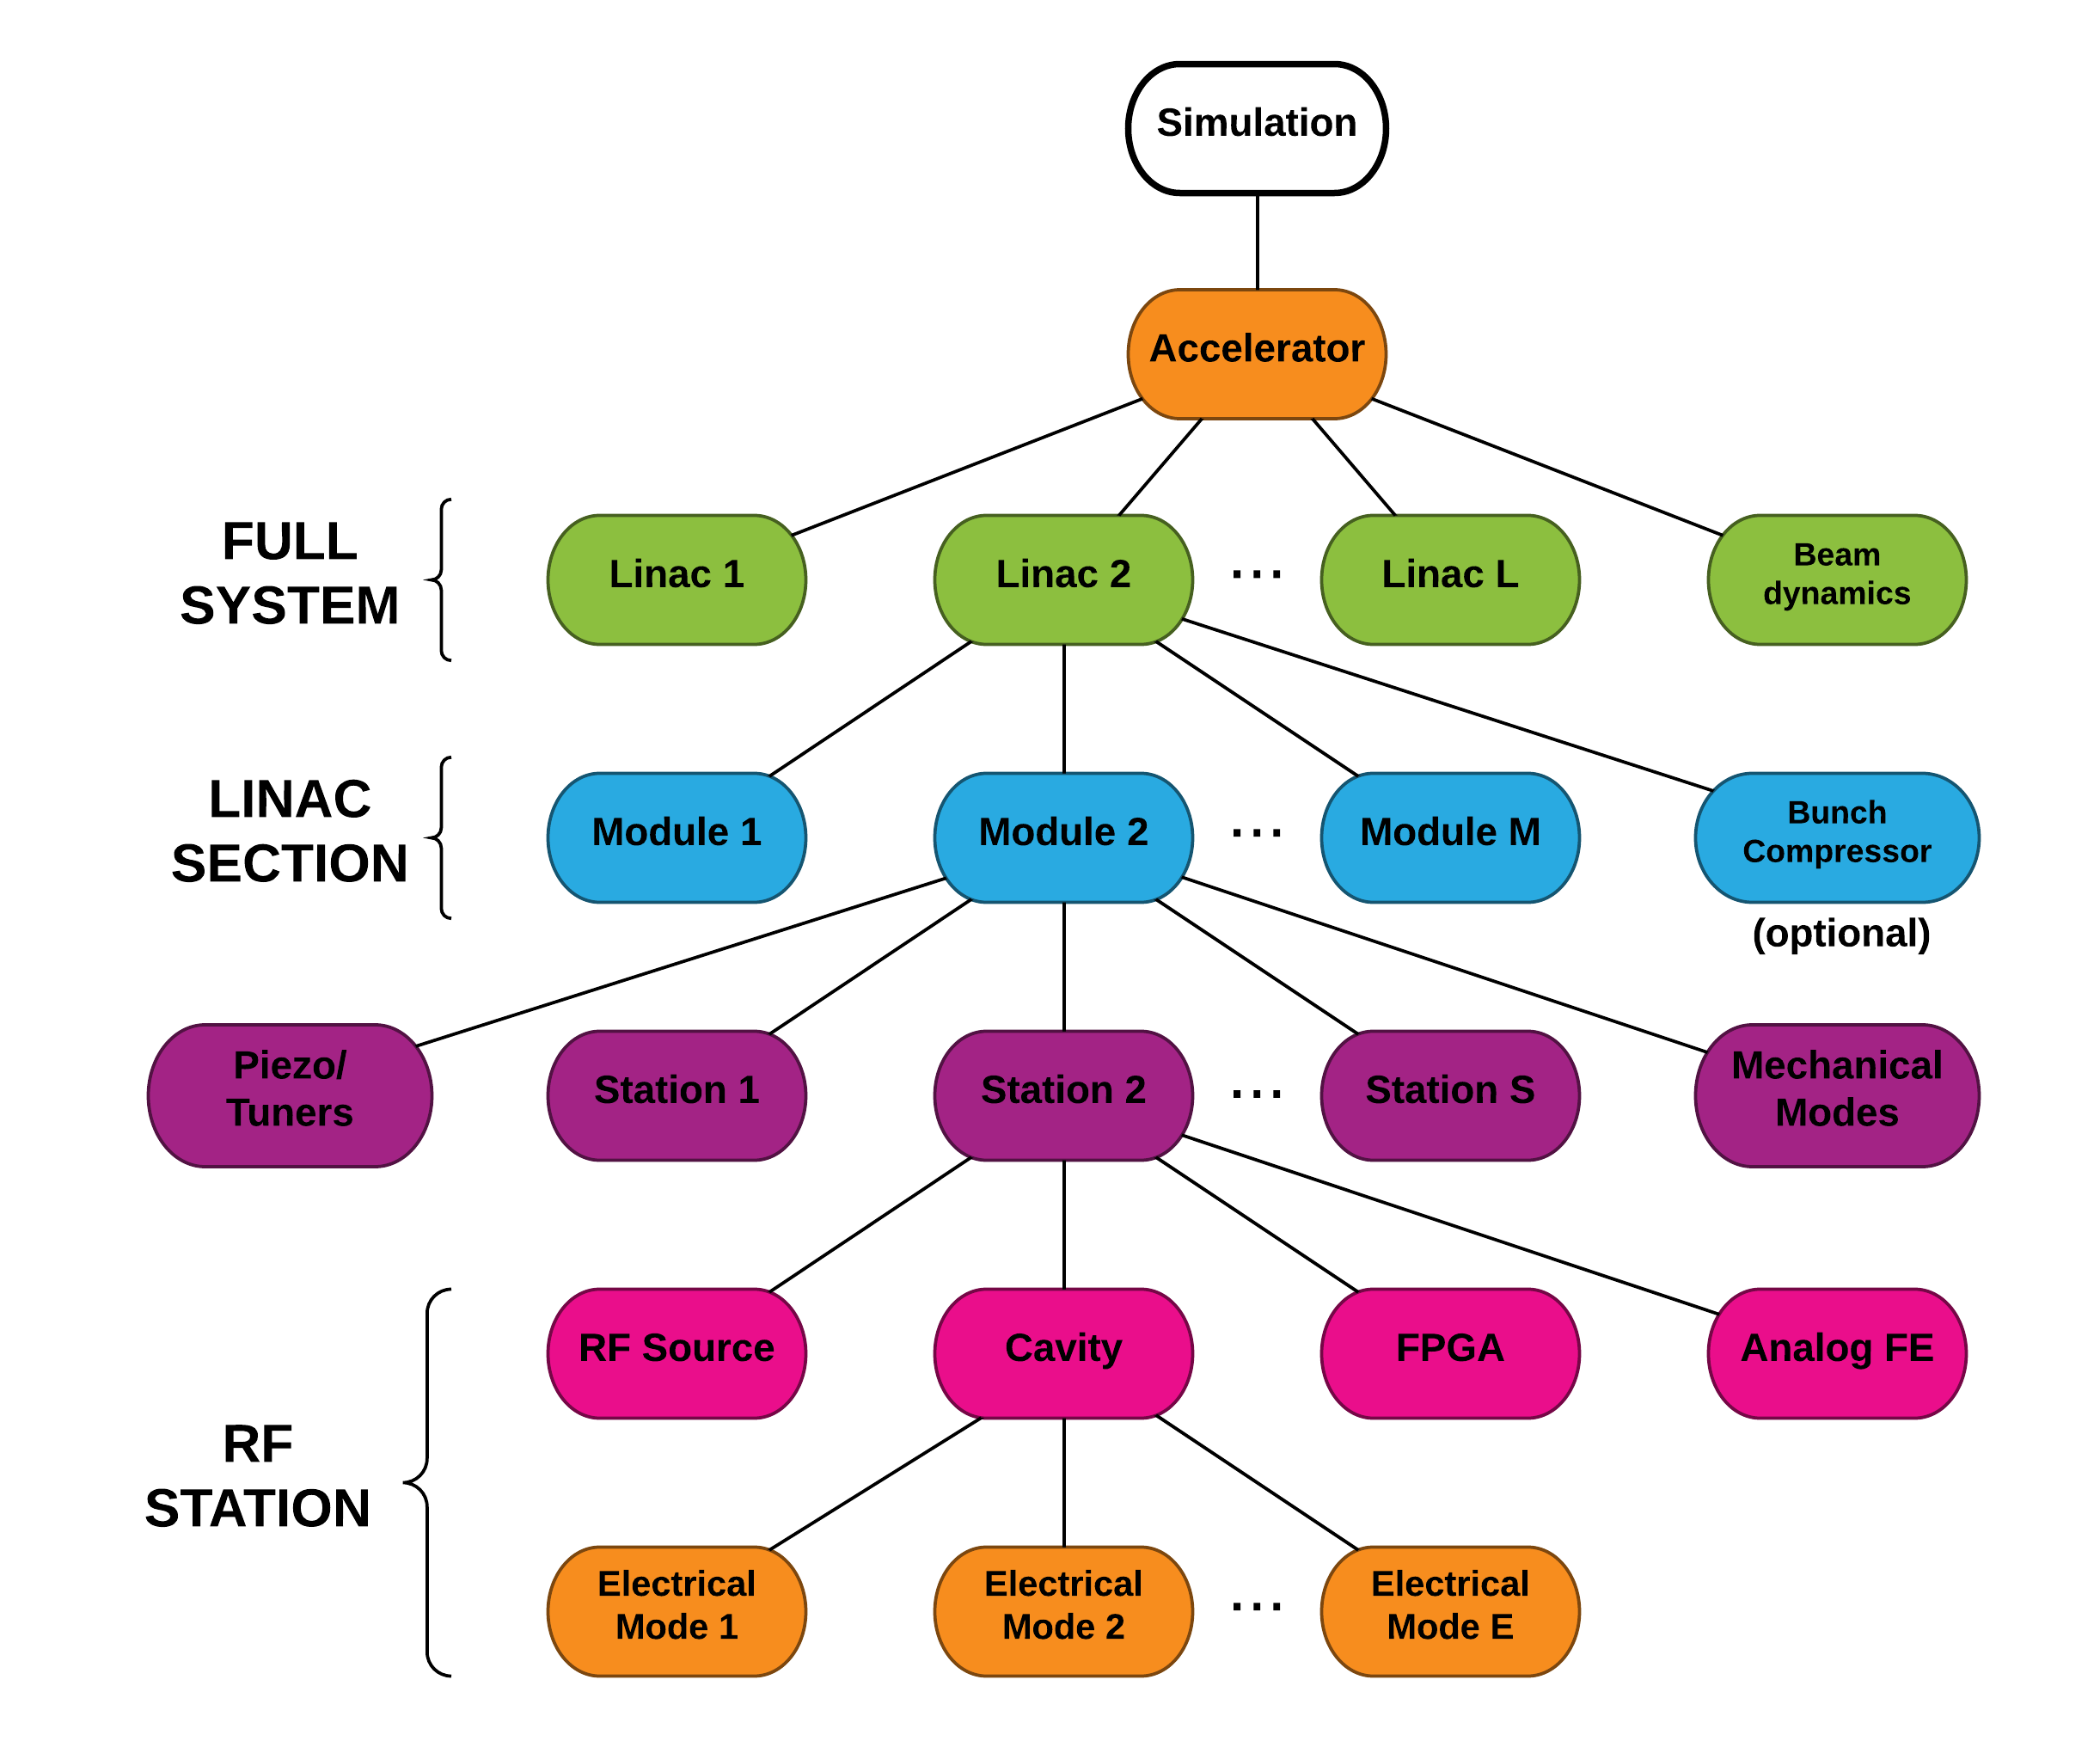
\includegraphics[scale=0.6]{../figures/Model_hierarchy.png}
\caption{Model hierarchy.}
\label{fig:model_hierarchy}
\end{figure}

The accelerator model is intended to be modular in order to adapt to different configurations. The motivation behind this partitioning is to allow for different types of studies. For example, one can focus on some localized effects at the RF station level where only one station is simulated, or inspect how different cavities interact mechanically inside a cryomodule, or run studies at a machine level in order to analyze slow beam-based feedback performance where not much detail on the internals of RF stations is desired.

The different model configurations described above are put in practice using a model hierarchy shown in Figure~\ref{fig:model_hierarchy}. The first component is a simulation entity, which describes simulation parameters such as time step size, total simulation time, etc. The simulation then includes an accelerator which can be composed of one or more Linac sections, including a longitudinal beam dynamics simulation to represent beam propagating from one Linac section to the next. One linac section is then represented as a series of cryomodules, optionally followed by a bunch compressor. This is the fundamental building block of the accelerator, where one can imagine to have the case of L1 in Fig.~\ref{fig:lclsII-feedback_layout} with two cryomodules and no bunch compressor, followed by HL (with different frequency, beam phase relative to the RF, etc), this time followed by a bunch compressor (BC1 in this case).

Each cryomodule is then represented by a collection of RF stations, including inter-station interactions through a model of the mechanical resonances in the cryomodule. The electro-mechanical couplings between the mechanical eigenmodes and individual electrical eigenmodes in the cavities are represented, as well as the effect of tuners and piezos on the mechanical resonances. Each RF station is composed of the typical RF system components, with an N-cell cavity (including a configurable number of normal modes), a high-power RF source, an FPGA controller, and the analog front-end (which represents anti-alias filtering, LLRF noise, etc). The last stage of the hierarchy is the cavity electrical eigenmodes, which each have their own resonance frequency, Qs and couplings with mechanical modes in a cryomodule.

In the next few sections we describe the models used in each layer of the hierarchy shown in Fig.~\ref{fig:model_hierarchy}, starting bottom up so that the reader progressively understands every component in each layer without making any assumptions.

\newpage

\section{RF Station}
\label{sec:rf_station}

\begin{figure}
\centering
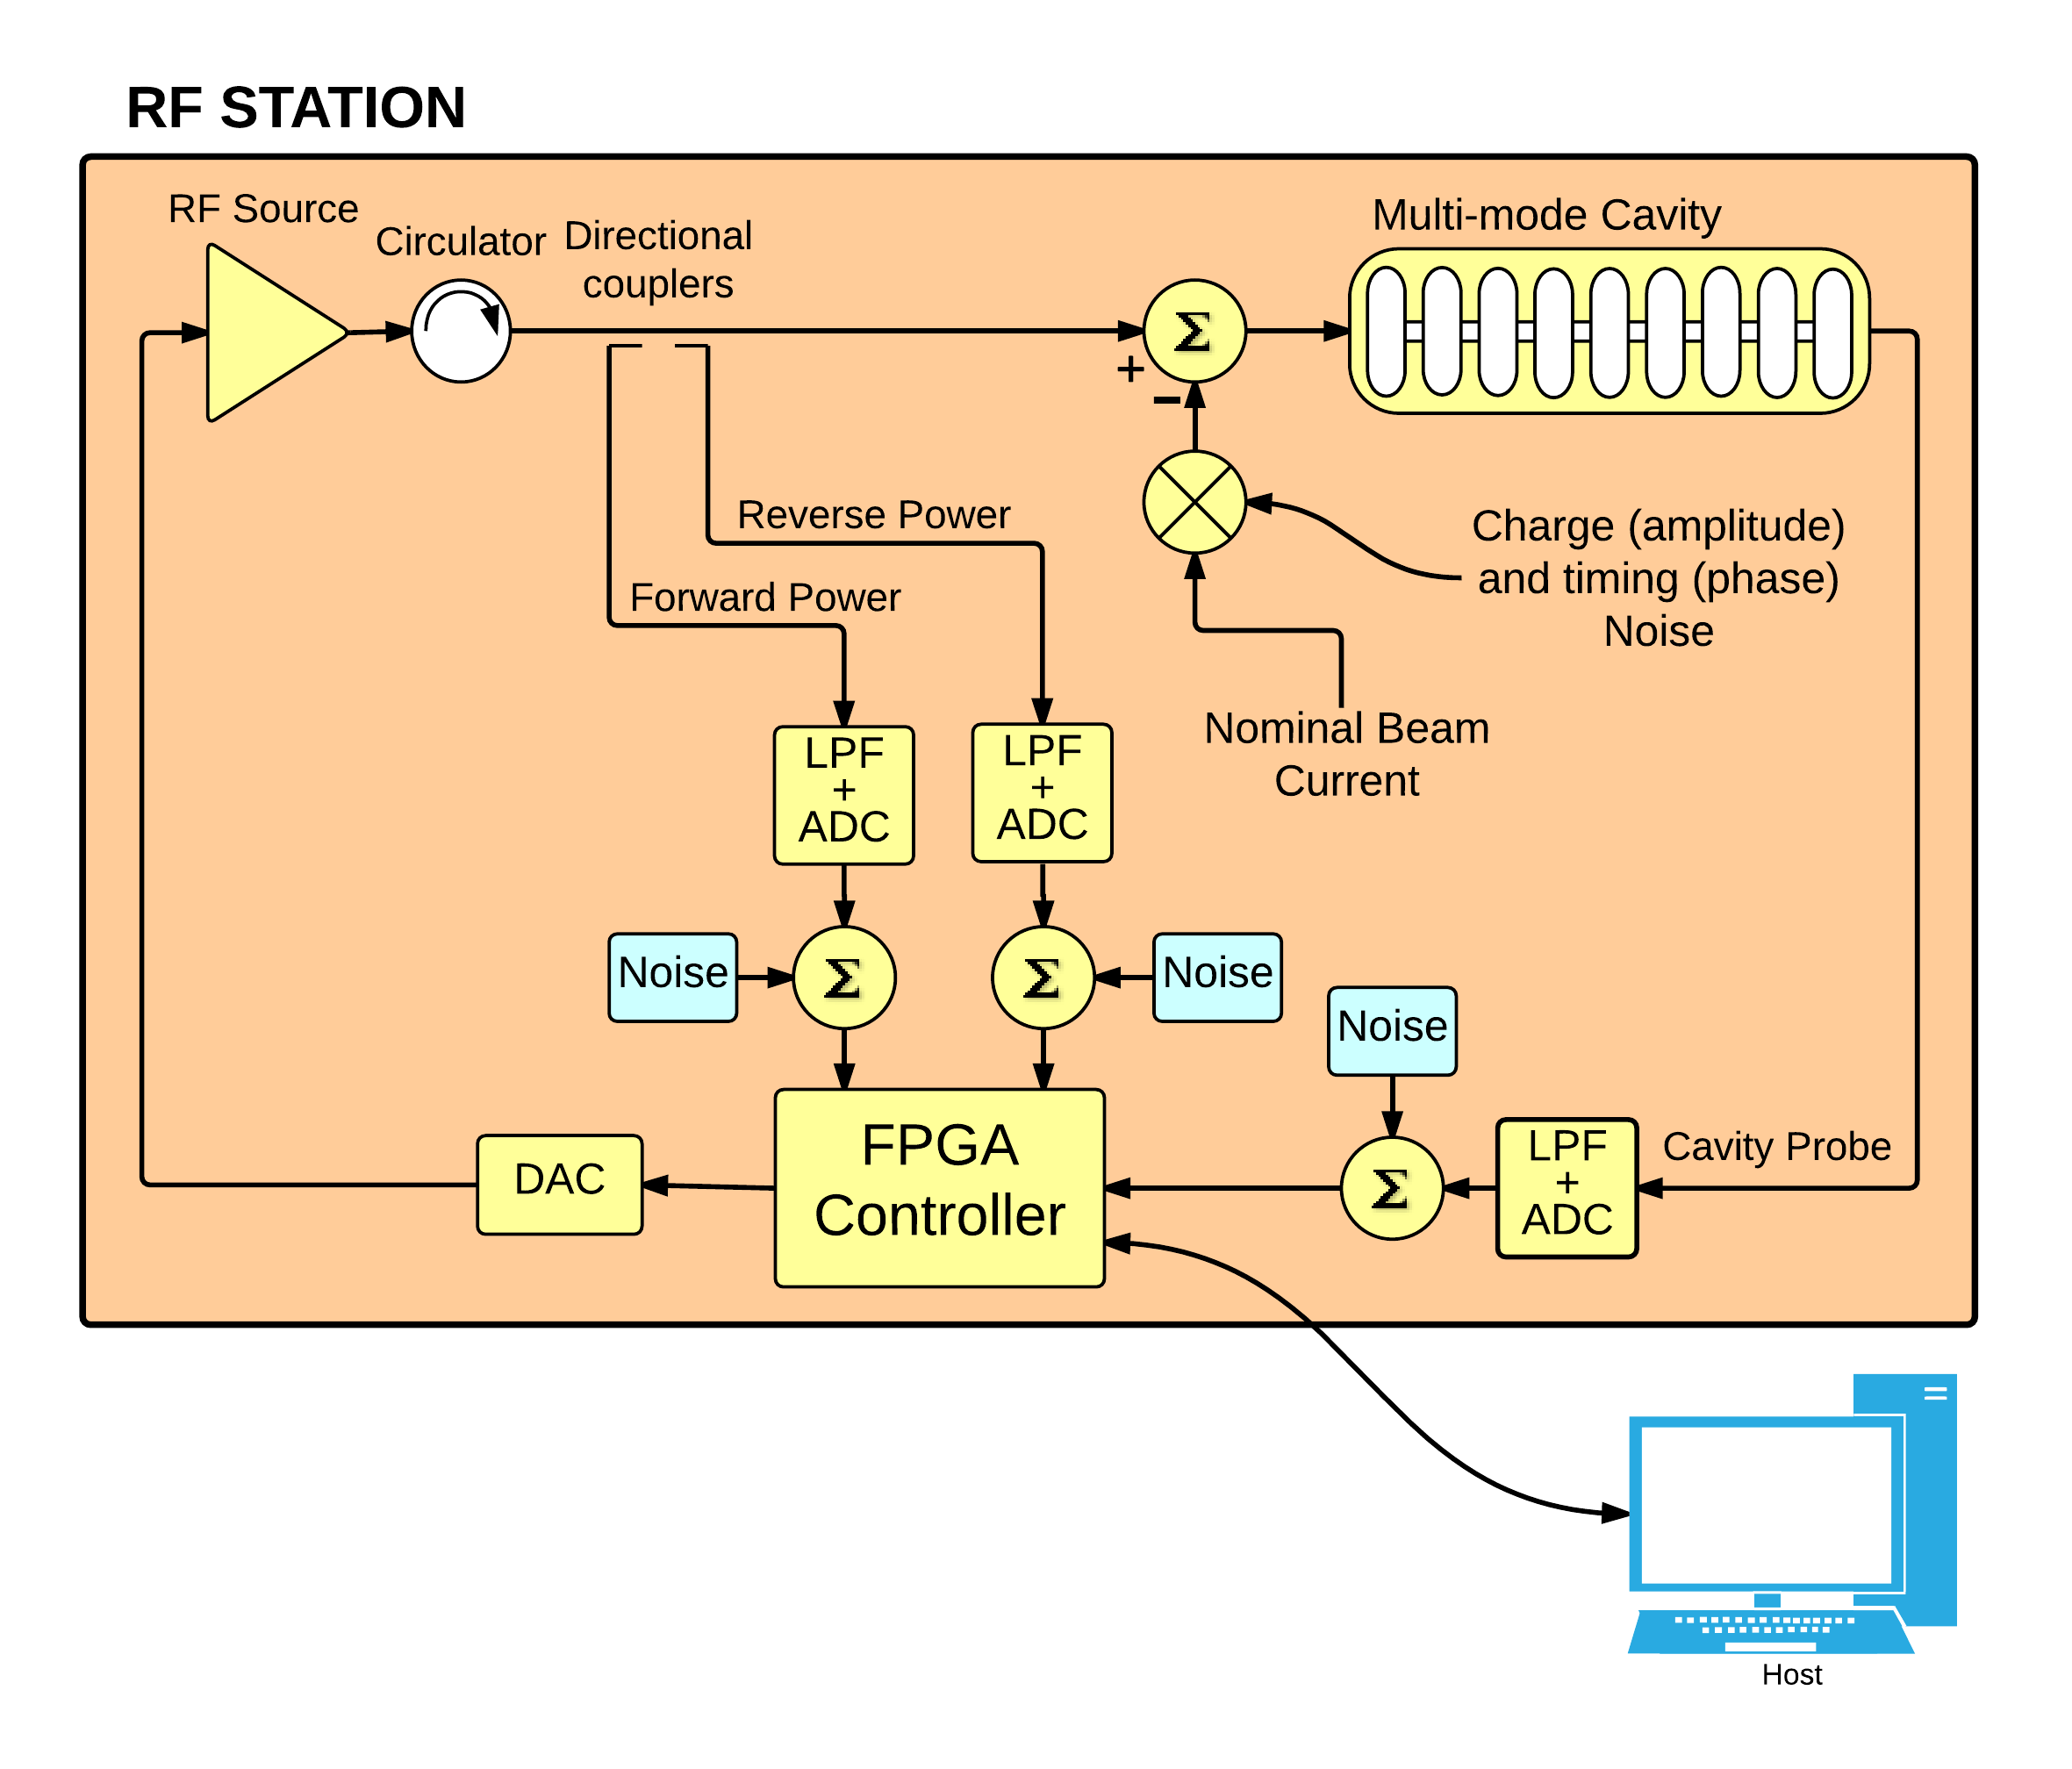
\includegraphics[scale=0.75]{../figures/Station_rf_blocks.png}
\caption{RF Station block diagram.}
\label{fig:Station_block_diagram}
\end{figure}

The RF station model includes a multi-cell cavity (including different normal modes, detuning and their different couplings), an FPGA controller, a saturation model for the RF source, filters, etc. The RF station is modeled at baseband, where up and down conversions in the real system are not considered and only the slowly varying amplitude and phase modulations (or In-phase and Quadrature, I\&Q) of a carrier at the RF reference frequency are represented. The FPGA controller in a real system typically works on I-Q sampled cavity fields. Representing the rest of the components in the RF station model at baseband allows for a more computationally efficient implementation of the simulation code, while not losing information of interest on the different complex signals. This approximation will be specifically demonstrated when describing the cavity model equations.

The RF station model responds to the typical RF system topology, with an FPGA-based system controlling the EM field inside an accelerating cavity as shown in Fig.~\ref{fig:Station_block_diagram}. It also includes the cavity-beam interaction through beam loading, as well as different noise sources, which can be either correlated or non-correlated. The different components of the RF station model are described in the rest of this section.

\subsection{Cavity model}

From EM theory, we know $\vec{E}$ and $\vec{B}$ fields inside a cavity can be broken down into independent eigenmodes (independent solutions to Maxwell's equations inside a cavity or waveguide). For a 9-cell cavity, the highest $\vec{E}$ field along the cavity axis is obtained for the $\pi$-mode. Ideally we would like to only excite that mode applying the proper input signal, which is only is known from theory. However, this is hard to achieve in practice as some other modes are present due to geometrical errors in the cavity shape or further deformation due to mechanical forces that are generated.

The cavity model described here responds to a multi-cell cavity structure, with couplings to the RF source, a cavity field probe and the beam. There are two aspects to representing this problem: the complete EM field description inside the cavity and the equivalent circuit representation, where the field description is needed in order to define the equivalent circuit using simulation codes like Superfish~\cite{ref:superfish}. It is convenient to use the equivalent circuit representation in order to model the cavity behavior as well as its interactions with the RF system and the beam.

Ideally, we would like to measure the EM fields from each mode present in the cavity in order to control them appropriately. However, the best  we can do is measure the overall field in the cavity, designated here by $\vec E_{\rm probe}$. It is measured in practice using a probe antenna, and is theoretically given by

\begin{equation}
  \vec E_{\rm probe} = \sum_{\mu} \vec{V}_{\mu} /\sqrt{Q_{\rm p_{\mu}}(R/Q)_{\mu}}
  \label{eq:E_probe}
\end{equation}

\noindent where $\vec{V}_{\mu}$ is a representative measure of the energy stored in each electrical mode $\mu$, designated as mode cavity voltage, and where $Q_{\rm p_{\mu}}(R/Q)_{\mu}$ is the coupling impedance of the probe port for that mode.

Alternatively, the expression for reverse (a.k.a.~reflected) wave travelling outward from the fundamental port includes a prompt reflection term, yielding

\begin{equation}
  \vec E_{\rm reverse}=\sum_\mu \vec V_\mu / \sqrt{Q_{g_{\mu}}(R/Q)_\mu} - \vec K_g
  \label{eq:E_reverse}
\end{equation}

\noindent where $Q_{g_{\mu}}(R/Q)_\mu$ is the coupling impedance of the drive port of mode $\mu$.

\subsubsection{Electromagnetic eigenmode}

\begin{figure}
\centering
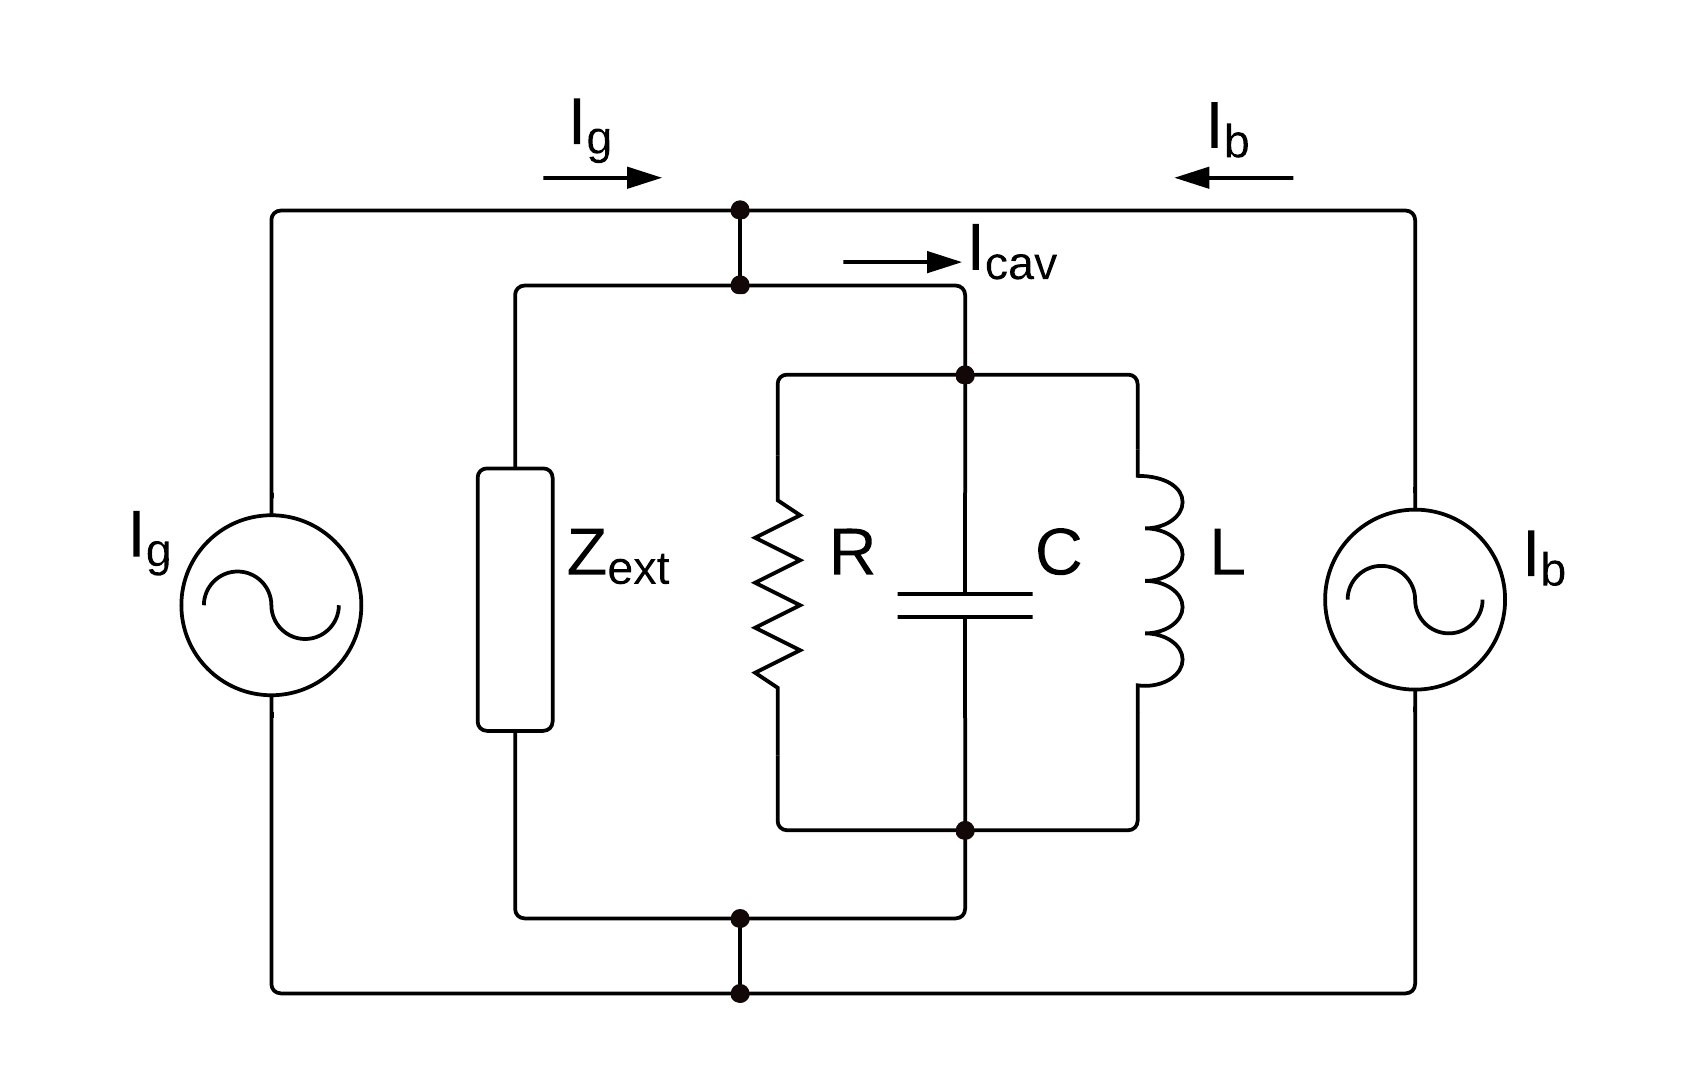
\includegraphics[scale=0.20]{../figures/cavity_eq_circuit.png}
\caption{Electromagnetic eigenmode equivalent circuit.}
\label{fig:cav_eq_circuit}
\end{figure}

A multi-cell cavity is represented by a series of coupled resonators (one per cell in the cavity), each represented by an RLC circuit~\cite{ref:montgomery}. Decomposing the EM cavity fields into eigenmodes and applying the principle of superposition we obtain the representation expressed by equation~\ref{eq:E_probe}~\cite{ref:cell_modes}. The equivalent circuit used to represent one cavity mode is shown in Fig.~\ref{fig:cav_eq_circuit}, where each mode's accelerating voltage is added in order to obtain the cavity overall accelerating voltage, as deduced from Equation~\ref{eq:E_probe}. Each mode has its own value of $\vec V$, $(R/Q)$, $Q_x$, and other characteristics that will be introduced later.

If we apply Kirchhoff's current law to the mode's RLC equivalent circuit (see figure~\ref{fig:cav_eq_circuit}, $\mu$ refers to a particular eigenmode), we get:

\begin{equation}
  \centering \vec I_{\mu} = \vec I_{\rm C_{\mu}} + \vec I_{\rm R_{\mu}} + \vec I_{\rm L_{\mu}}
  \label{eq:currents}
\end{equation}

\noindent where:

\begin{equation}
  \frac{d\vec I_{\rm C_{\mu}}}{dt} = C_{\mu} \cdot \frac{d^2\vec V_{\mu}}{dt^2}\text{,}\qquad \frac{d\vec I_{\rm R_{\mu}}}{dt} = \frac{1}{R_{\rm L_{\mu}}}\frac{d\vec V_{\mu}}{dt} \qquad \text{and}\qquad \frac{d\vec I_{\rm L_{\mu}}}{dt} = \vec V_{\mu}/L_{\mu}
  \label{eq:currents2}
\end{equation}

Differentiating both sides of equation~\ref{eq:currents} and substituting using eq.~\ref{eq:currents2}, the full vector (complex) differential equation for the cavity accelerating voltage $\vec V_{\mu}$ can be written as:

\begin{equation}
  \frac{d^2\vec V_{\mu}}{dt^2} + \frac{1}{R_{\rm L_{\mu}}C_{\mu}}\frac{d\vec V_{\mu}}{dt} + \frac{1}{L_{\mu}C_{\mu}}\vec V_{\mu} = \frac{1}{C_{\mu}}\frac{d\vec I_{\mu}}{dt}
\end{equation}

\noindent which can be expressed as a function of the mode's nominal resonance frequency $\omega_{0_{\mu}}$ ($1/L_{\mu}C_{\mu}=\omega_{0_{\mu}}^2$) and loaded Q ($1/R_{\rm L_{\mu}}C_{\mu}=\omega_{0_{\mu}}/Q_{\rm L_{\mu}}$):
 
\begin{equation}
  \frac{d^2\vec V_{\mu}}{dt^2} + \frac{\omega_{0_{\mu}}}{Q_{\rm L_{\mu}}}\frac{d\vec V_{\mu}}{dt} + \omega_{0_{\mu}}^2 \vec V_{\mu} = \frac{\omega_{0_{\mu}}^2 R_{\rm L_{\mu}}}{Q_{\rm L_{\mu}}}\frac{d\vec I_{\mu}}{dt}
  \label{eq:2nd_order}
\end{equation}

Taking the slowly varying envelope approximation~\cite{ref:svea} ($\omega_{f_{\mu}} \ll \omega_{0_{\mu}}$), separating voltage and current into real and imaginary parts, assuming that the detune frequency varies slowly with respect to the carrier frequency ($\omega_{d_{\mu}} \ll \omega_{0_{\mu}}$) and that $Q_{\rm L_{\mu}} \gg 1$, we can reduce the order of equation~\ref{eq:2nd_order} (a second-order band-pass filter centered at the resonance frequency) to a first-order low-pass filter at baseband~\cite{ref:schilcher}:

\begin{equation}
  \left(1-j\frac{\omega_{d_{\mu}}}{\omega_{f_{\mu}}}\right)\vec V_{\mu} + \frac{1}{\omega_{f_{\mu}}}\frac{d\vec V_{\mu}}{dt} = R_{\rm L_{\mu}} \vec I_{\mu}
  \label{eq:1st_order1}
\end{equation}

\noindent where $\omega_{f_{\mu}}=\omega_{0_{\mu}}/2Q_{L_{\mu}}$ is the mode's bandwidth and $\omega_{d_{\mu}}=2\pi\Delta f_{\mu}$ is the (time varying) detune frequency, given as $\omega_{d_{\mu}}=\omega_{0_{\mu}}-\omega_{ref}$, {\it i.e.}, the difference between actual eigenmode frequency $\omega_{0_{\mu}}$ and the accelerator's time base $\omega_{\rm ref}$.

Transposing the cavity drive term into a combination of the RF source incident wave and beam loading (opposite sign indicating energy absorption by the beam), we can express eq.~\ref{eq:1st_order1} as:

\begin{equation}
  \left(1-j\frac{\omega_{d_{\mu}}}{\omega_{f_{\mu}}}\right)\vec V_{\mu} + {\frac{1}{\omega_{f_{\mu}}}}\frac{d\vec V_{\mu}}{dt} =  2\vec K_{\rm g}\sqrt{R_{\rm g_{\mu}}} - R_{\rm b_{\mu}}\vec I_{\rm beam}
  \label{eq:1st_order2}
\end{equation}

\noindent where $\vec K_{\rm g}$ is the incident wave amplitude in $\sqrt{\rm Watts}$, $R_{\rm g_{\mu}}=Q_{\rm g_{\mu}}(R/Q)_{\mu}$ is the coupling impedance of the drive port, $\vec I_{\rm beam}$ is the beam current, and $R_{\rm b_{\mu}}=Q_{\rm L_{\mu}}(R/Q)_{\mu}$ is the coupling impedance to the beam.

The overall $Q_{\rm L_{\mu}}$ is given as $1/Q_{\rm L_{\mu}}=1/Q_{0_{\mu}}+1/Q_{g_{\mu}}+1/Q_{p_{\mu}}$, where $1/Q_{0_{\mu}}$ represents losses to the cavity walls, $1/Q_{g_{\mu}}$ represents coupling to the input coupler, and $1/Q_{p_{\mu}}$ represents coupling to the field probe. $(R/Q)_{\mu}$ is the shunt impedance of the mode in Ohms, a pure geometry term computable for each particular eigenmode using E\&M codes like Superfish. Physically, shunt impedance relates a mode's stored energy $U_{\mu}$ to the accelerating voltage it produces, according to 

\begin{equation}
  U_{\mu} = \frac{V_{\mu}^2}{(R/Q)_{\mu}\omega_{0_{\mu}}}
\end{equation}

The only assumptions in the above formulation are that the cavity losses are purely resistive, and thus expressible with a fixed $Q_{0_{\mu}}$, and that no power is launched into the cavity from the field probe.  If other ports have incoming power, there would be additional terms of the same form as $2\vec K_g\sqrt{R_g}$.

The $\frac{\omega_{d_\mu}}{\omega_{f}}\vec{V}_{\mu}$ term in \ref{eq:1st_order2} will be relatively small compared to the other terms. To appropriately take it into account it is better to isolate it by defining  a vector $\vec{S}_{\mu}$ such that:

\begin{equation}
\vec{V}_{\mu} = \vec{S}_{\mu}e^{j\theta_{\mu}}
\label{eq:V_mu}
\end{equation}

\begin{equation}
\frac{d\theta_{\mu}}{dt} = \omega_{d_\mu}
\label{eq: d0_dt}
\end{equation}

\noindent yielding:

\begin{equation}
\left(1 - j\frac{\omega_{d_\mu}}{\omega_{f_{\mu}}}\right)\vec{S}_{\mu}e^{j\theta_{\mu}} + \frac{1}{\omega_{f_{\mu}}}
    \left(\frac{d\vec{S}_{\mu}}{dt}e^{j\theta_{\mu}} + \vec{S}_{\mu} \cdot j\omega_{d_{\mu}}e^{j\theta_{\mu}}\right) = 2\vec{K}_{g}\sqrt{R_{g_{\mu}}} - R_{b_{\mu}}\vec{I}_{\rm beam}
\label{eq Gov_S}
\end{equation}

\noindent The governing equation for the mode's accelerating voltage can thus be written as a set of two first order differential equations (eqs.~\ref{eq: dS_dt} and~\ref{eq: d0_dt}):

\begin{equation}
  \frac{d\vec{S}_{\mu}}{dt} = -\omega_{f_{\mu}}\vec{S}_{\mu} + \omega_{f_{\mu}}e^{-j\theta_{\mu}}\left(2\vec{K}_g\sqrt{R_{g_{\mu}}} 
    - R_{b_{\mu}}\vec{I}_{\rm beam} \right)
\label{eq: dS_dt}
\end{equation}

Note that this state-variable equation is a pure low-pass filter, an advantage especially in the FPGA implementation.

\subsubsection{Software implementation}

\begin{figure}
\centering
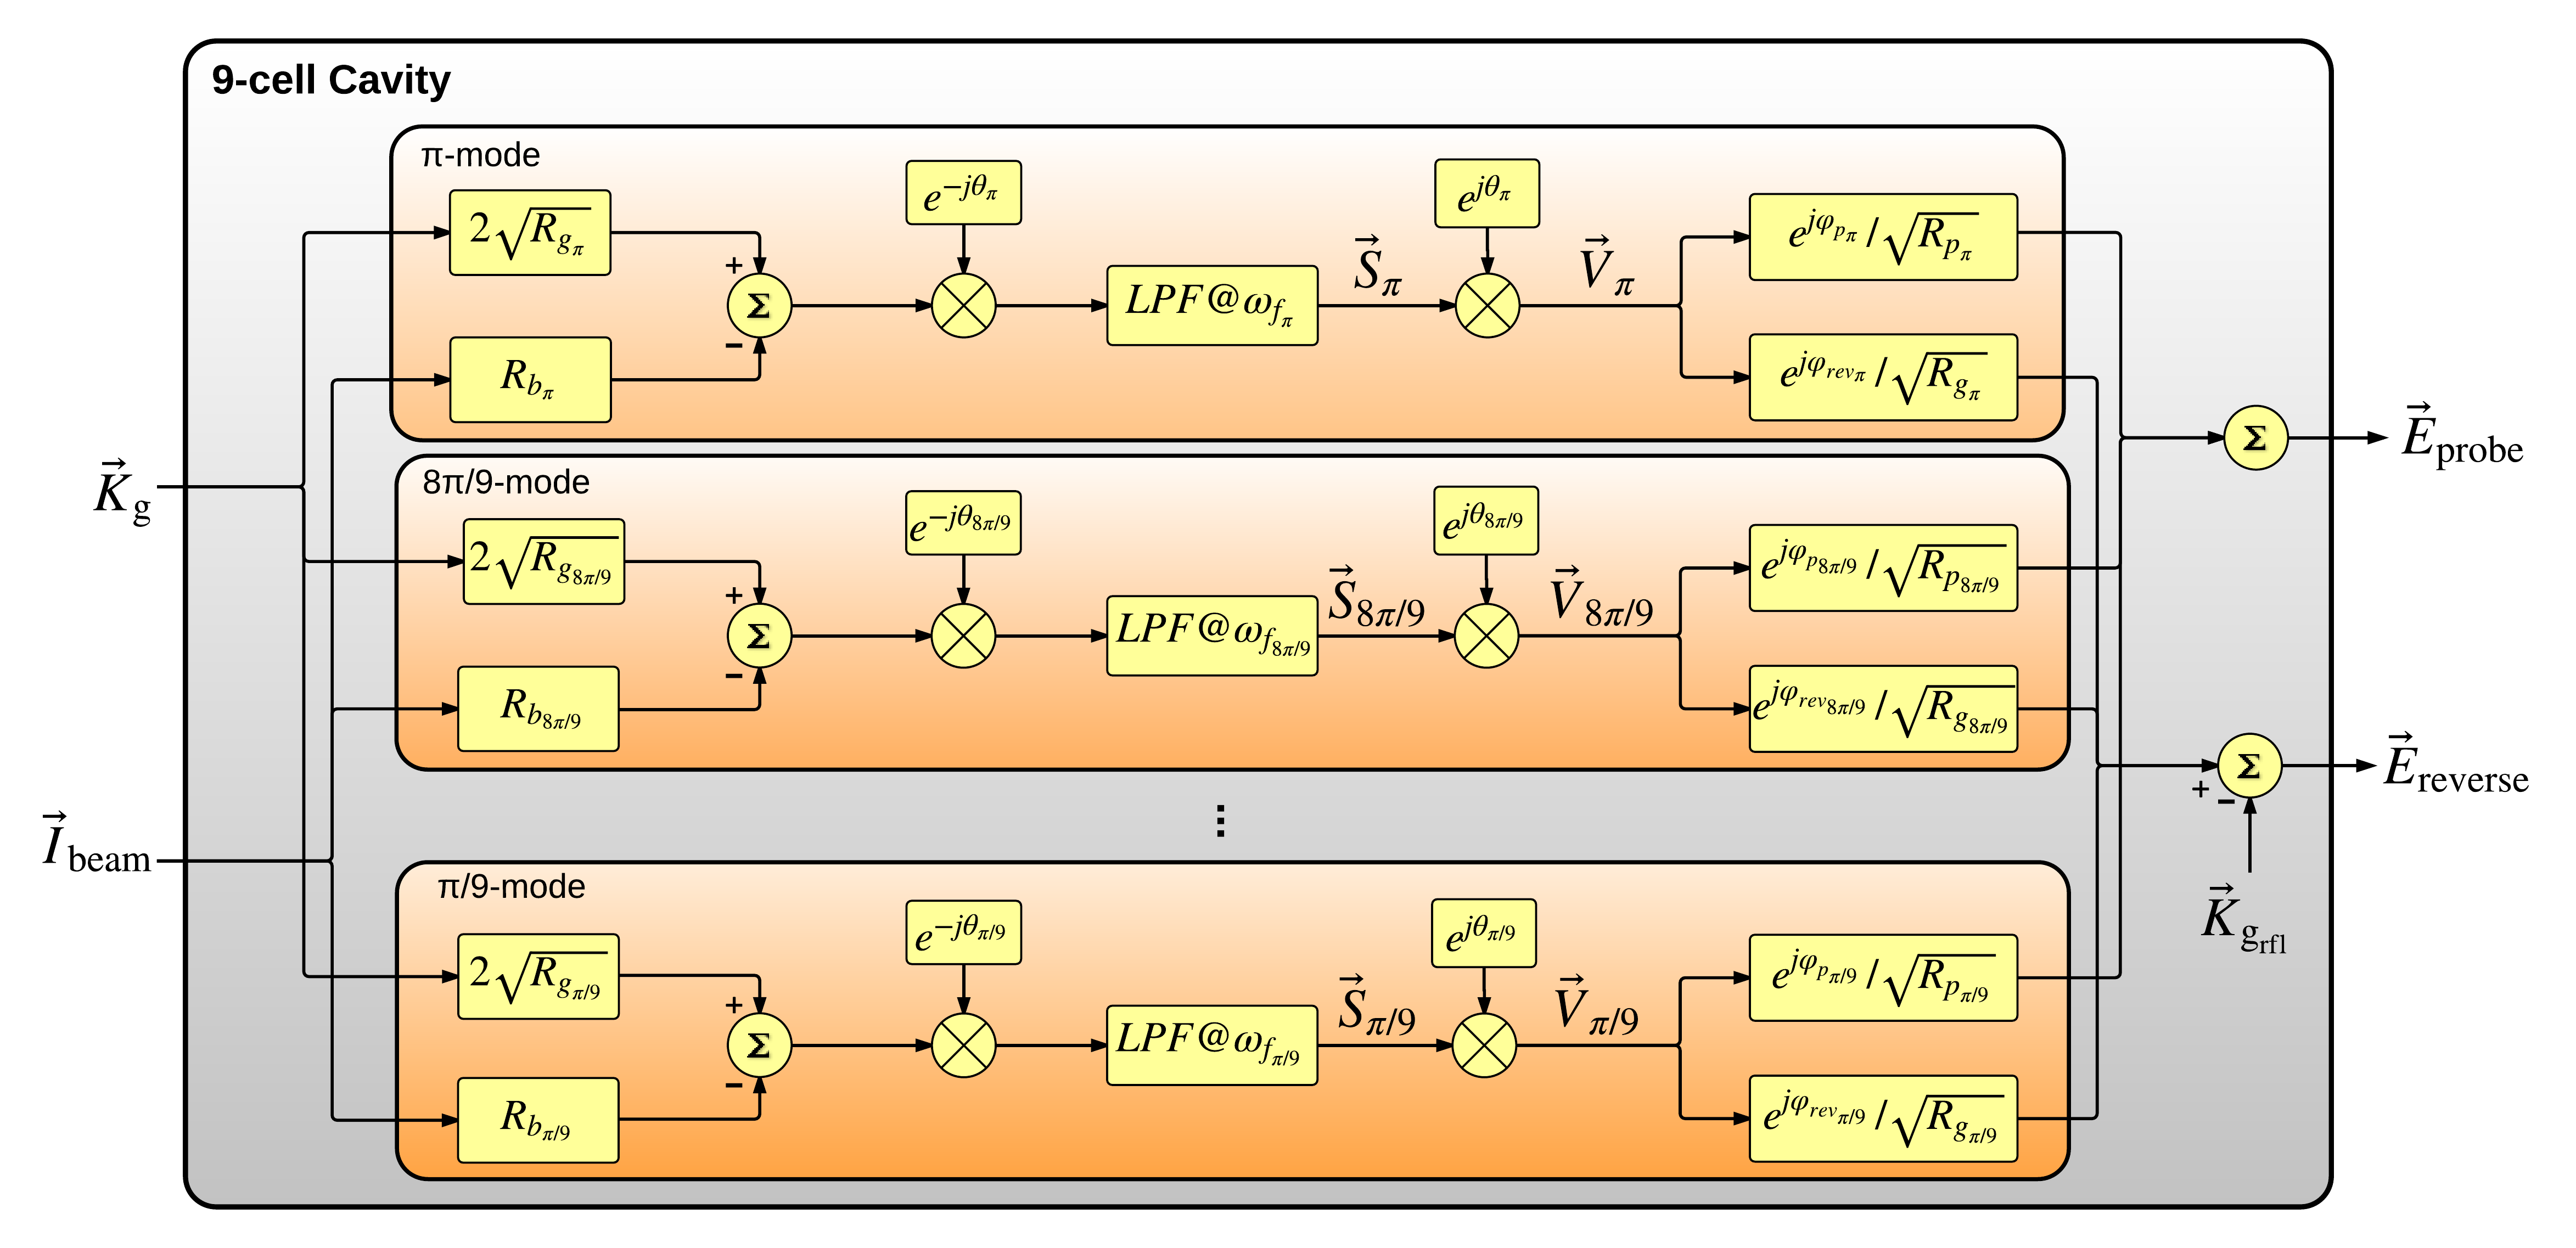
\includegraphics[scale=0.4]{../figures/Cavity_modes.png}
\caption{Data path for the computation of a 9-cell cavity model.}
\label{fig:RF_cavity_block_diagram}
\end{figure}

We started this section with the definition of $\vec E_{\rm probe}$ and $\vec E_{\rm reverse}$ (see Fig.~\ref{fig:Station_block_diagram}), given by equations \ref{eq:E_probe} and \ref{eq:E_reverse} respectively. These equations express the measured probe and reverse fields as a function of eigenmode voltages ($\vec V_\mu$) and their respective port couplings. We also defined the state-variable equation governing the accelerating voltage for each eigenmode in Equation~\ref{eq: dS_dt}, where $\vec{V}_{\mu} = \vec{S}_{\mu}e^{j\theta_{\mu}}$. We can therefore compute the cavity probe and reverse signals as a function of the incident wave $\vec K_{\rm g}$ and the beam current $\vec I_{\rm beam}$.

Figure~\ref{fig:RF_cavity_block_diagram} shows the data path implemented in software in order to compute the response of a nine-cell cavity (which can be configured for any type of cavity given the definition of the electrical eigenmodes and couplings). Each internal bock represents the implementation of Eq.~\ref{eq: dS_dt} for each eigenmode, and the summing junction at the end (taking the pre-factored eigenmode voltages) represents the computation of $\vec E_{\rm probe}$ and $\vec E_{\rm reverse}$ using Equations \ref{eq:E_probe} and \ref{eq:E_reverse}.

Note that there are two aspects represented in Fig.~\ref{fig:RF_cavity_block_diagram} which are not shown in the equations. The first one is the use of $\vec K_{\rm g_{rfl}}$ instead of $\vec K_{\rm g}$, as well as the terms $e^{j\varphi_{x}}$ in the factoring of each $\vec V_\mu$ term before the summing junctions. These terms represent frequency dependent propagation through cables and waveguides. In the case of the incident wave, if we define $TF_{\rm wg}(s)$ as the transfer function in Laplace domain of a wide-band filter representing the waveguide between the directional coupler on the high-power forward path and the cavity, we get:

\begin{equation}
 \vec K_{\rm g_{rfl}}(s) = \vec K_{\rm g}(s) \cdot TF_{\rm wg}(s)
\end{equation}

\noindent where the minus sign of the reflection on the cavity coupler is represented in the summing junction. This transformation takes into account the propagation of the reflection of the incident wave back to the directional coupler.
The cavity probe and reverse path also follow a similar transformation but in this case represented by a phase shift through the coaxial cable from the cavity probe and reverse ports and their respective ADCs in the LLRF. These phase shifts are represented by the $e^{j\varphi_{\rm rev_{\mu}}}$ and $e^{j\varphi_{\rm p_{\mu}}}$ terms in Fig.~\ref{fig:RF_cavity_block_diagram}, which are frequency dependent due to dispersion in the coaxial cables, and therefore need to be applied at this stage of the computation (before the summing junction).

The second aspect which has not been covered yet is the numerical discretization of the first-order low-pass filter in the cavity response, represented by the blocks labeled $LPF@\omega_{f_{\mu}}$ in Fig.~\ref{fig:RF_cavity_block_diagram}. The ODE integration is derived in Appendix~\ref{App:ODE_integration}, where Equation~\ref{eq: dS_dt} can be written as Equation~\ref{eq:exp_diff2}, where

\begin{equation}
 \vec V_{\rm out} = \vec S_{\mu} \mbox{ , } p = -\omega_f \mbox{ and, } \vec V_{\rm in} = e^{-j\theta_{\mu}} \left(2\vec{K}_g\sqrt{R_{g_{\mu}}} - R_{b_{\mu}}\vec{I}_{\rm beam}\right)
\end{equation}

\noindent as it can be deduced from Fig.~\ref{fig:RF_cavity_block_diagram}. This block solves for $\vec S_{\mu}$, which is transalated to the mode's accelerating voltage using equations~\ref{eq:V_mu} and~\ref{eq: d0_dt}, as indicated in the block diagram.

In summary, using the computations shown in Figure~\ref{fig:RF_cavity_block_diagram} (couplings, rotations, etc.) combined with the numerical discretization of the cavity filter described in Appendix~\ref{App:ODE_integration} applied every discrete simulation step, we can obtain time-series simulated data representing signal propagation through the multi-cell RF cavity, including the different eigenmodes and dispersion through cables and waveguides.

\subsubsection{Simulation results}

\begin{figure}
\centering
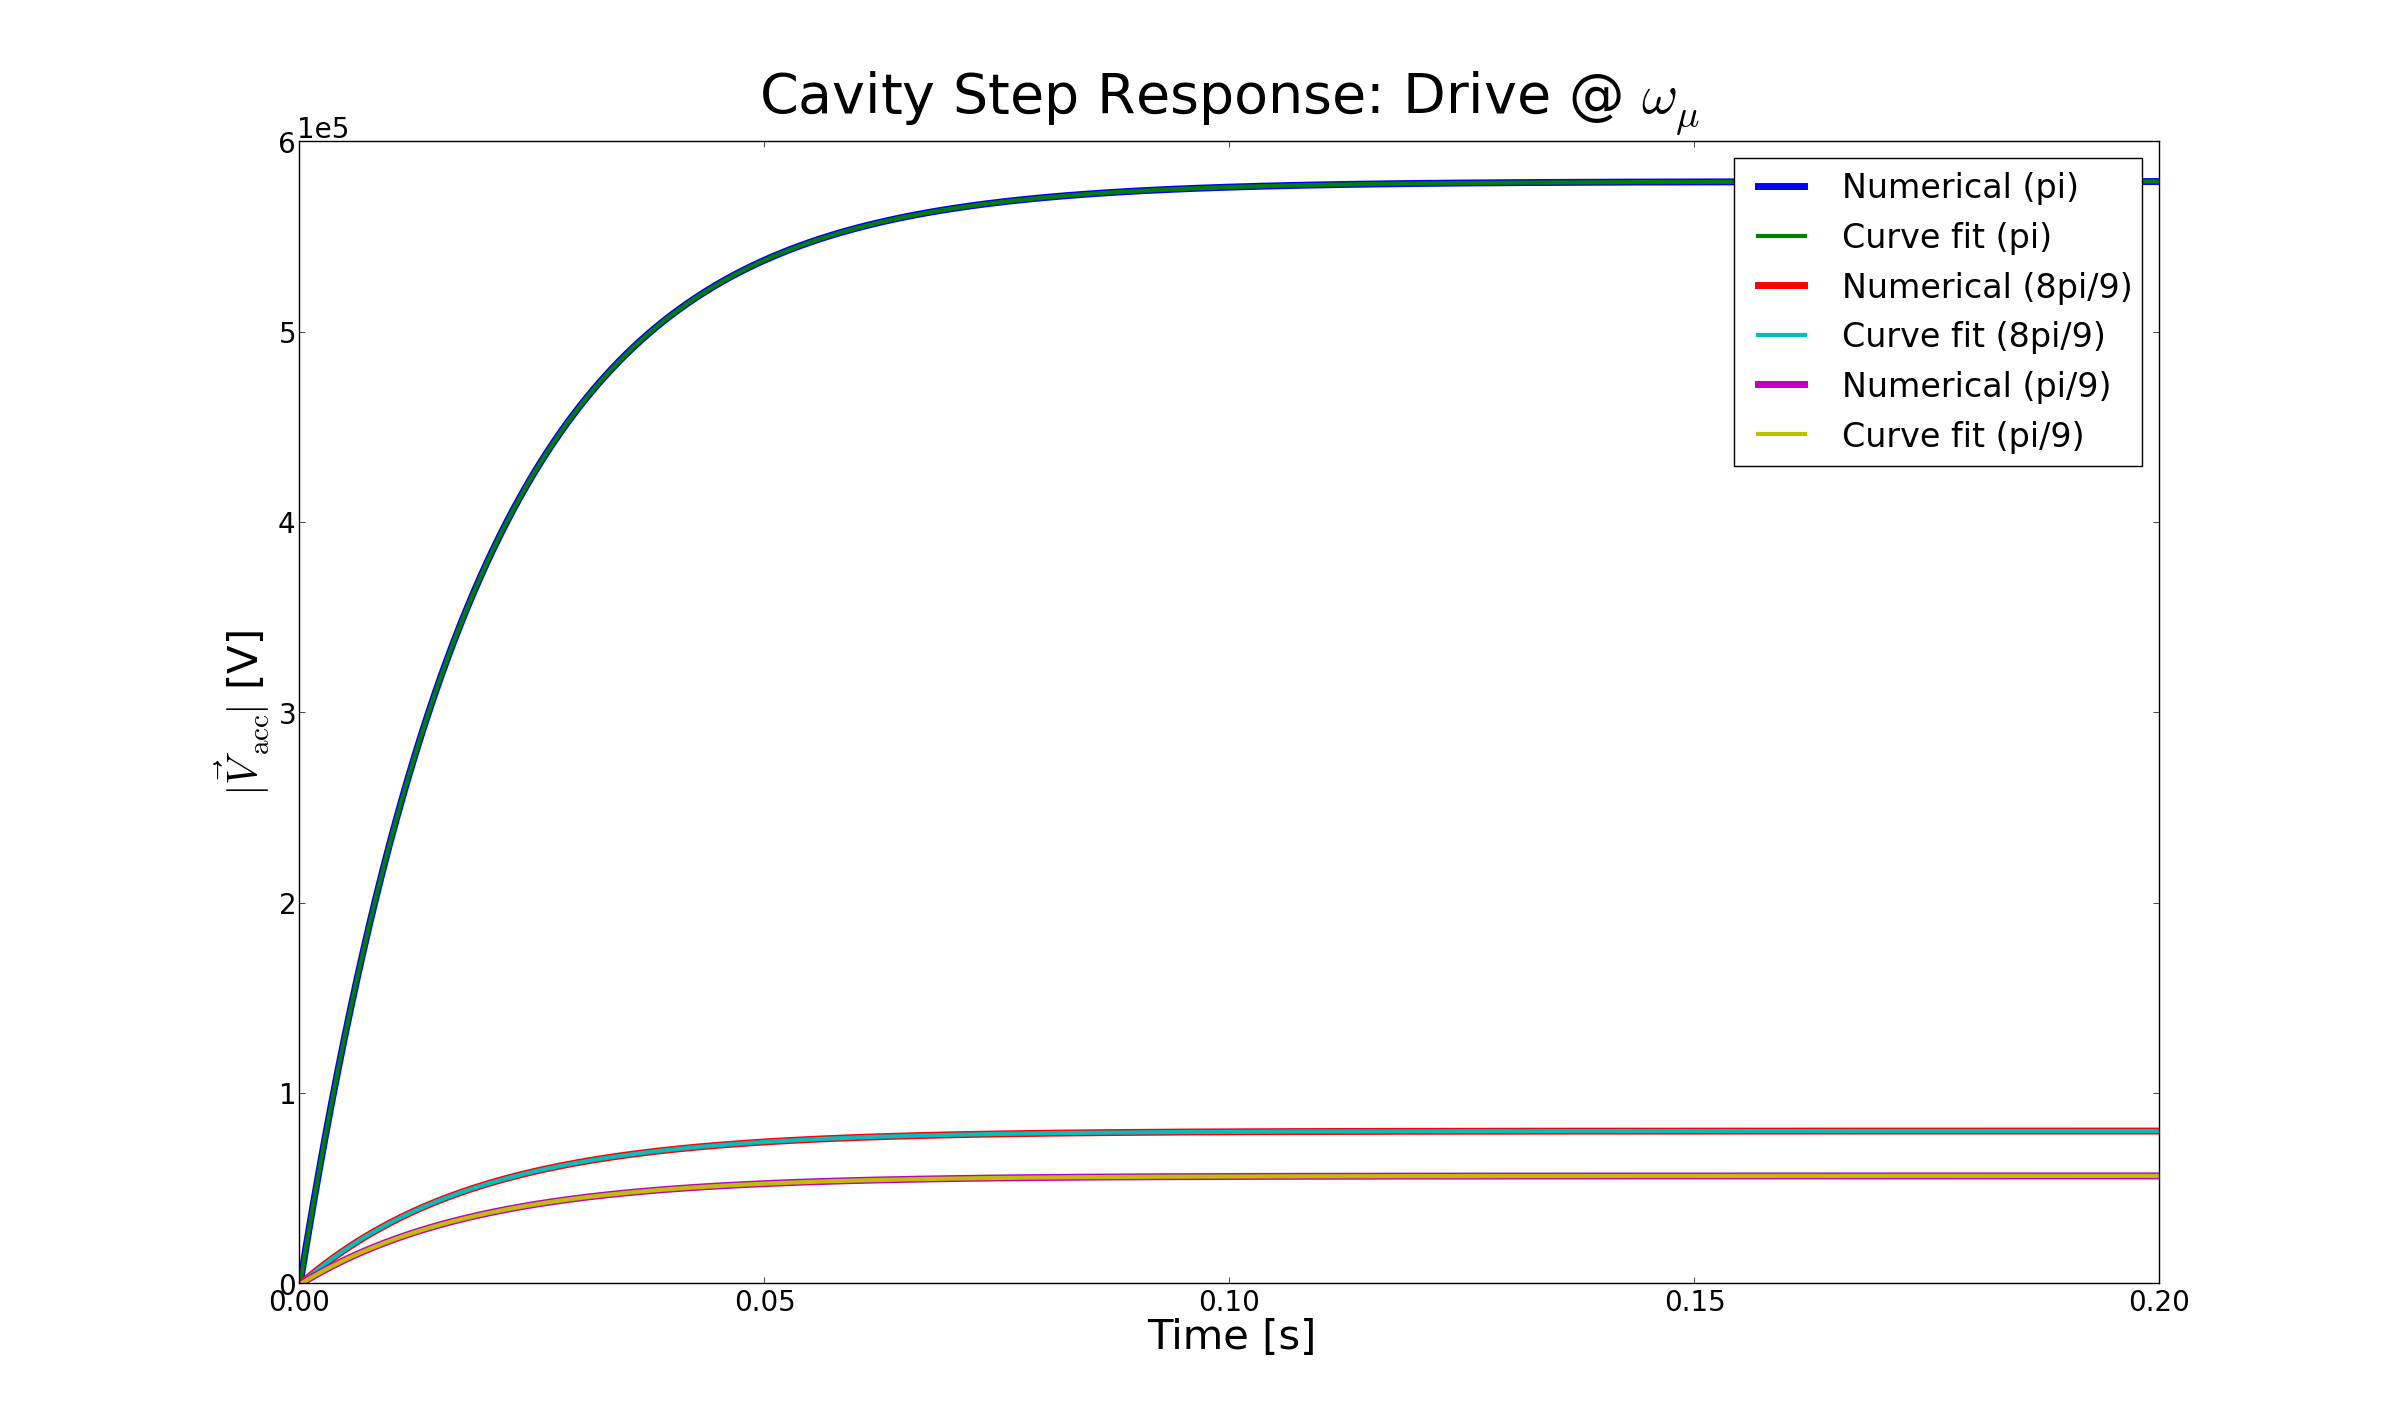
\includegraphics[scale=0.26]{../figures/cavity_test_drive.png}
\caption{Cavity unit test: Cavity response to a step function on the RF drive signal, where the input signal is at the each mode's resonance frequency.}
\label{fig:cav_step1}
\end{figure}

A few unit tests have been designed in order to check the correspondence between the numerical simulation results and the theoretical equations. The unit under test here is the cavity model illustrated in Fig.~\ref{fig:RF_cavity_block_diagram}. Some of these tests have little physical meaning and are even unrealizable in practice, however this is the beauty of the simulation world, where one can isolate effects in the calculations for different purposes, in this case in order to verify its own proper operation.

Figures~\ref{fig:cav_step1} and~\ref{fig:cav_step2} show the step response of three individual eigenmodes ($\pi$, $8\pi/9$ and $\pi/9$ modes in this case). In these tests, the cavity routine is configured to have one individual mode and the time-series simulation is run three times to obtain each one of the three curves on the plots. This allows us to fit the step response curves for each eigenmode individually, thus deducing mode bandwidths and couplings from the curve fit results. Both the numerical curves and the curve fits are shown for each simulation run, where (in the absence of noise as in this case) there is a very good correspondance between the two (in the order of $10^{-5}$ RMS errors).

\begin{figure}
\centering
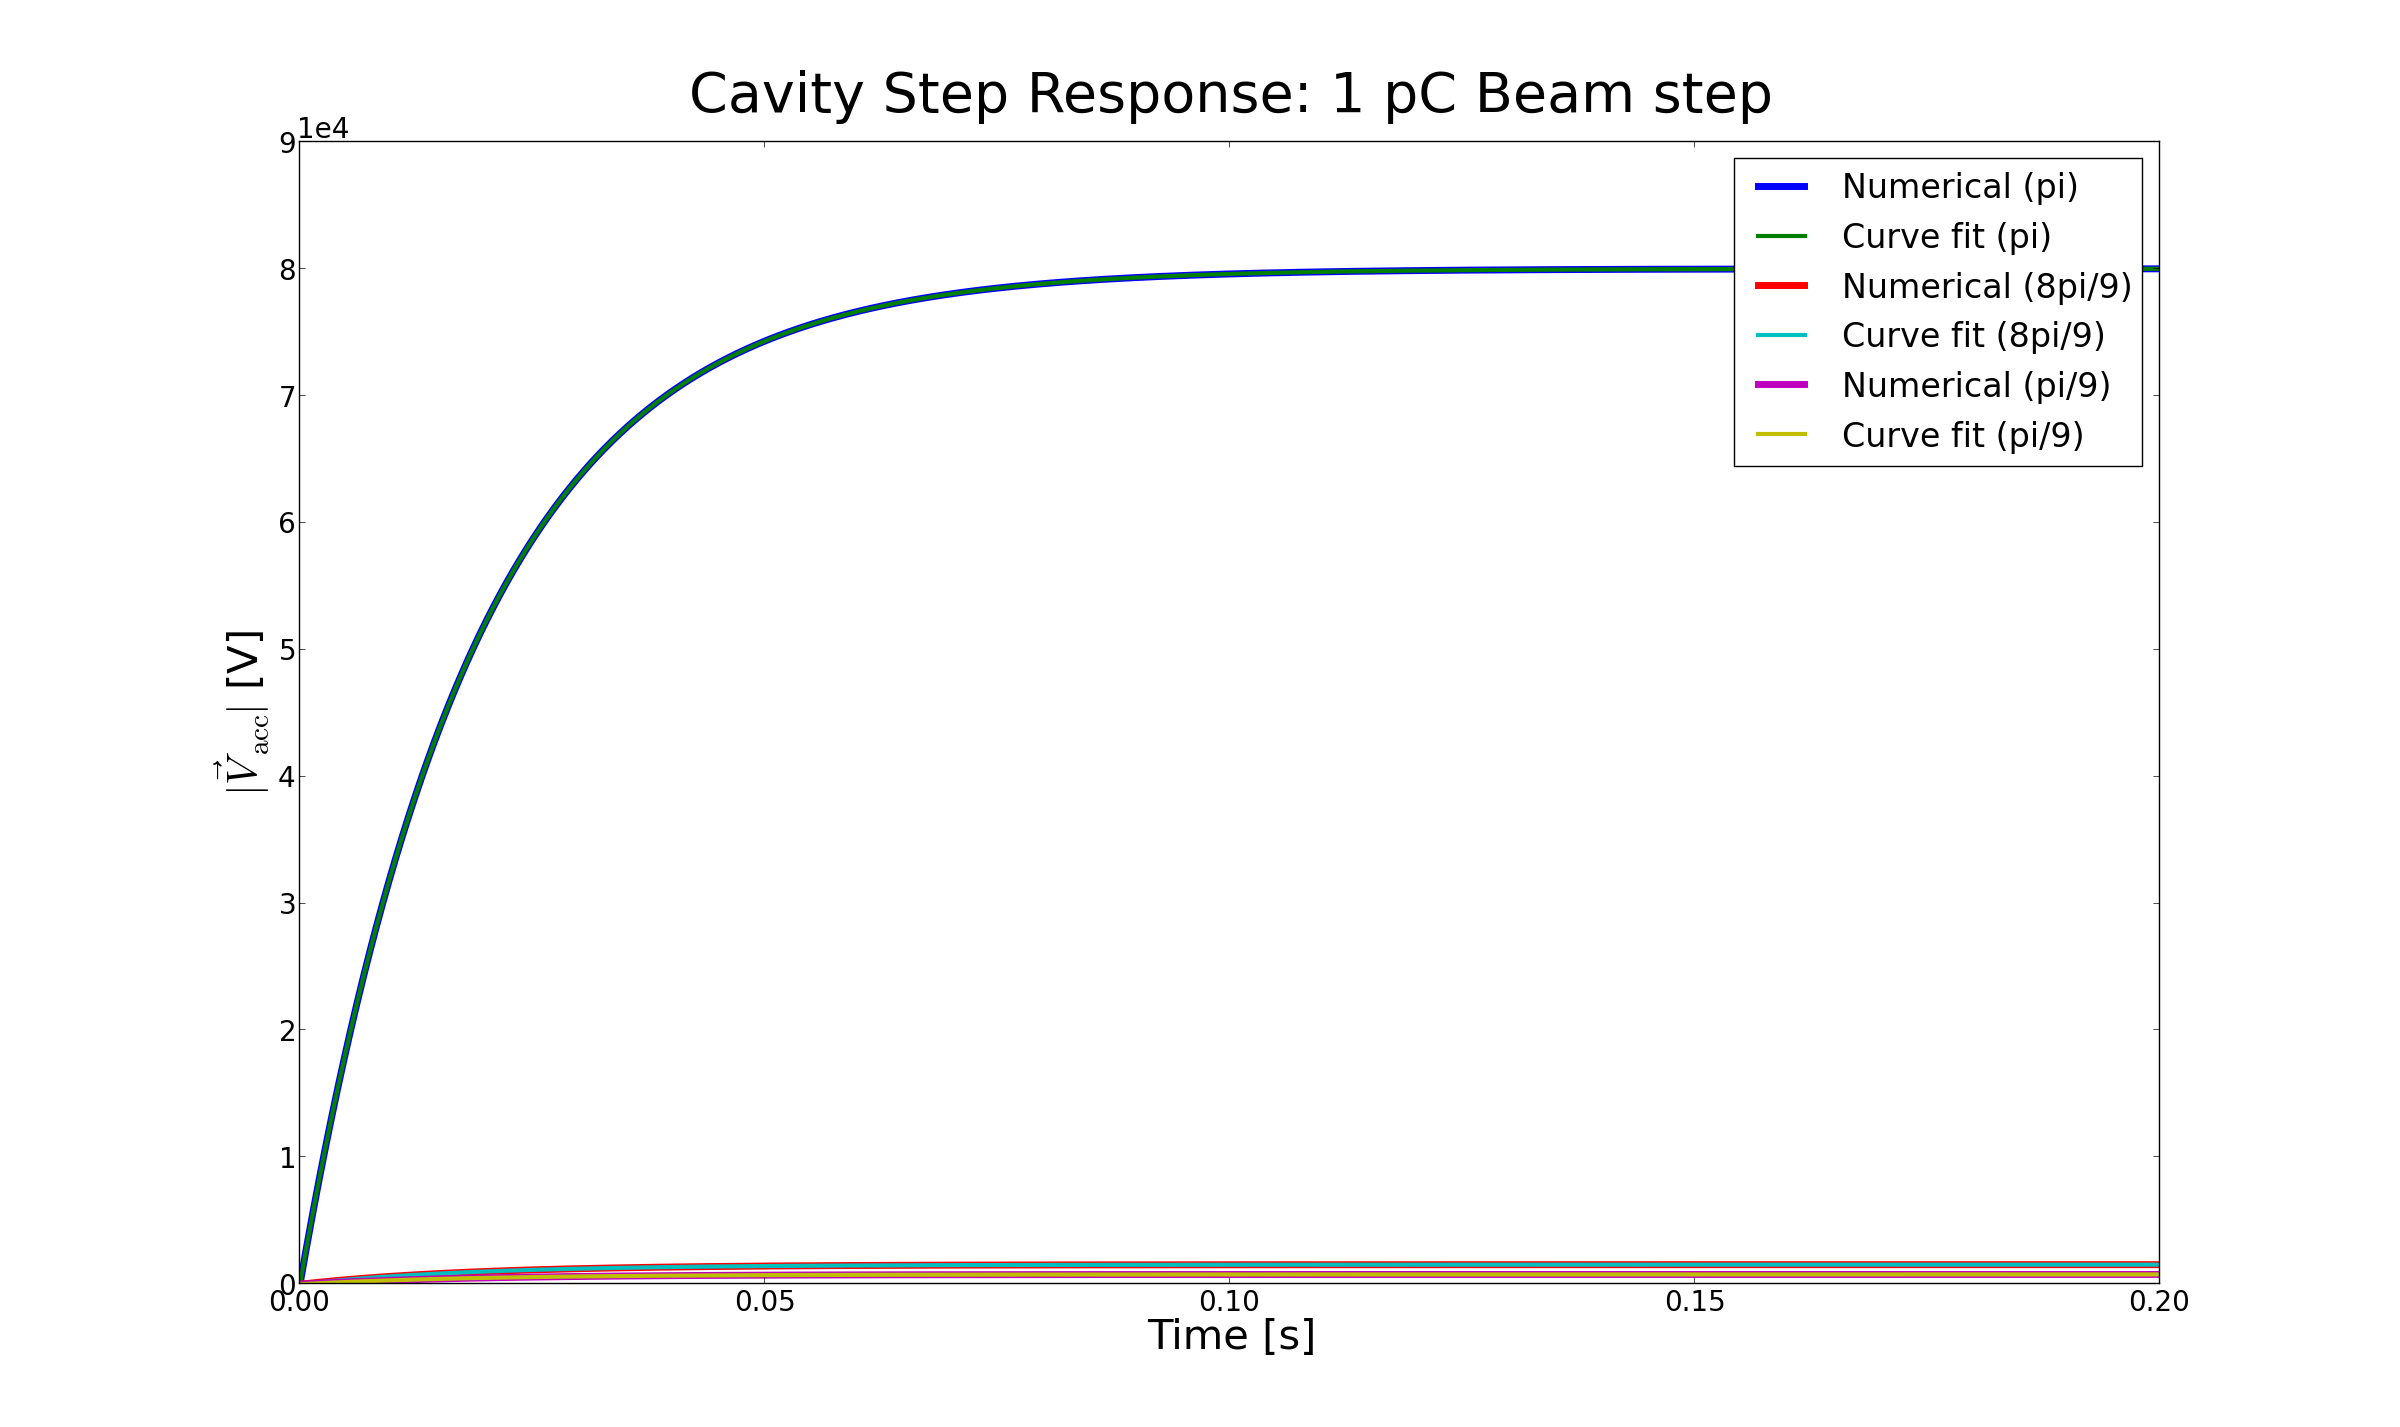
\includegraphics[scale=0.26]{../figures/cavity_test_beam.png}
\caption{Cavity unit test: Step response, beam coupling.}
\label{fig:cav_step2}
\end{figure}

In Fig.~\ref{fig:cav_step1} we introduce a unit amplitude step signal on the RF drive port at the mode's resonance frequency ($\omega_{0_{\mu}}$), which is equivalent to driving the input drive signal with a vector of unity length rotating at the mode's detune frequency ($\omega_{f_{\mu}}$). The input signals are then: $\vec K_{\rm g}=e^{j\theta_{\mu}}$ ($d\theta_{\mu}/dt = \omega_{d_\mu}$) and $\vec I_{\rm beam}=0$. As a result no ringing is observed. The model is designed to have unity gain at the mode's center frequency and one can therefore deduce couplings to the drive input by measuring the steady-state values. The step response is then fit to a 1st-order differential equation and the bandwidth of each mode is deduced, matching the configuration settings. This test provides a verification for the incident wave coupling impedance ($R_{\rm g_{\mu}}$ in eq.~\ref{eq: dS_dt}) as well as the mode's bandwidth ($\omega_{f_{\mu}}$ in the same equation).

In Fig.~\ref{fig:cav_step2} we introduce a step signal on the beam input signal equivalent to 1 pC beam charge (this number is just anecdotal since we are interested in measuring couplings, etc.). In this case $\vec K_{\rm g}=0$, providing means to deduce the beam coupling impedance for each eigenmode in a similar manner as described in the previous test. In both tests we also evaluate the probe ($\vec E_{\rm probe}$ in eq.~\ref{eq:E_probe}) and reverse field signals ($\vec E_{\rm reverse}$ in eq.~\ref{eq:E_reverse}) and compare them to the accelerating voltages, therefore being able to deduce the coupling impedances to the probe and drive ports for each eigenmode ($Q_{\rm p_{\mu}}(R/Q)_{\mu}$ and $Q_{g_{\mu}}(R/Q)_\mu$ in eqs.~\ref{eq:E_probe} and~\ref{eq:E_reverse} respectively).

\begin{figure}
\centering
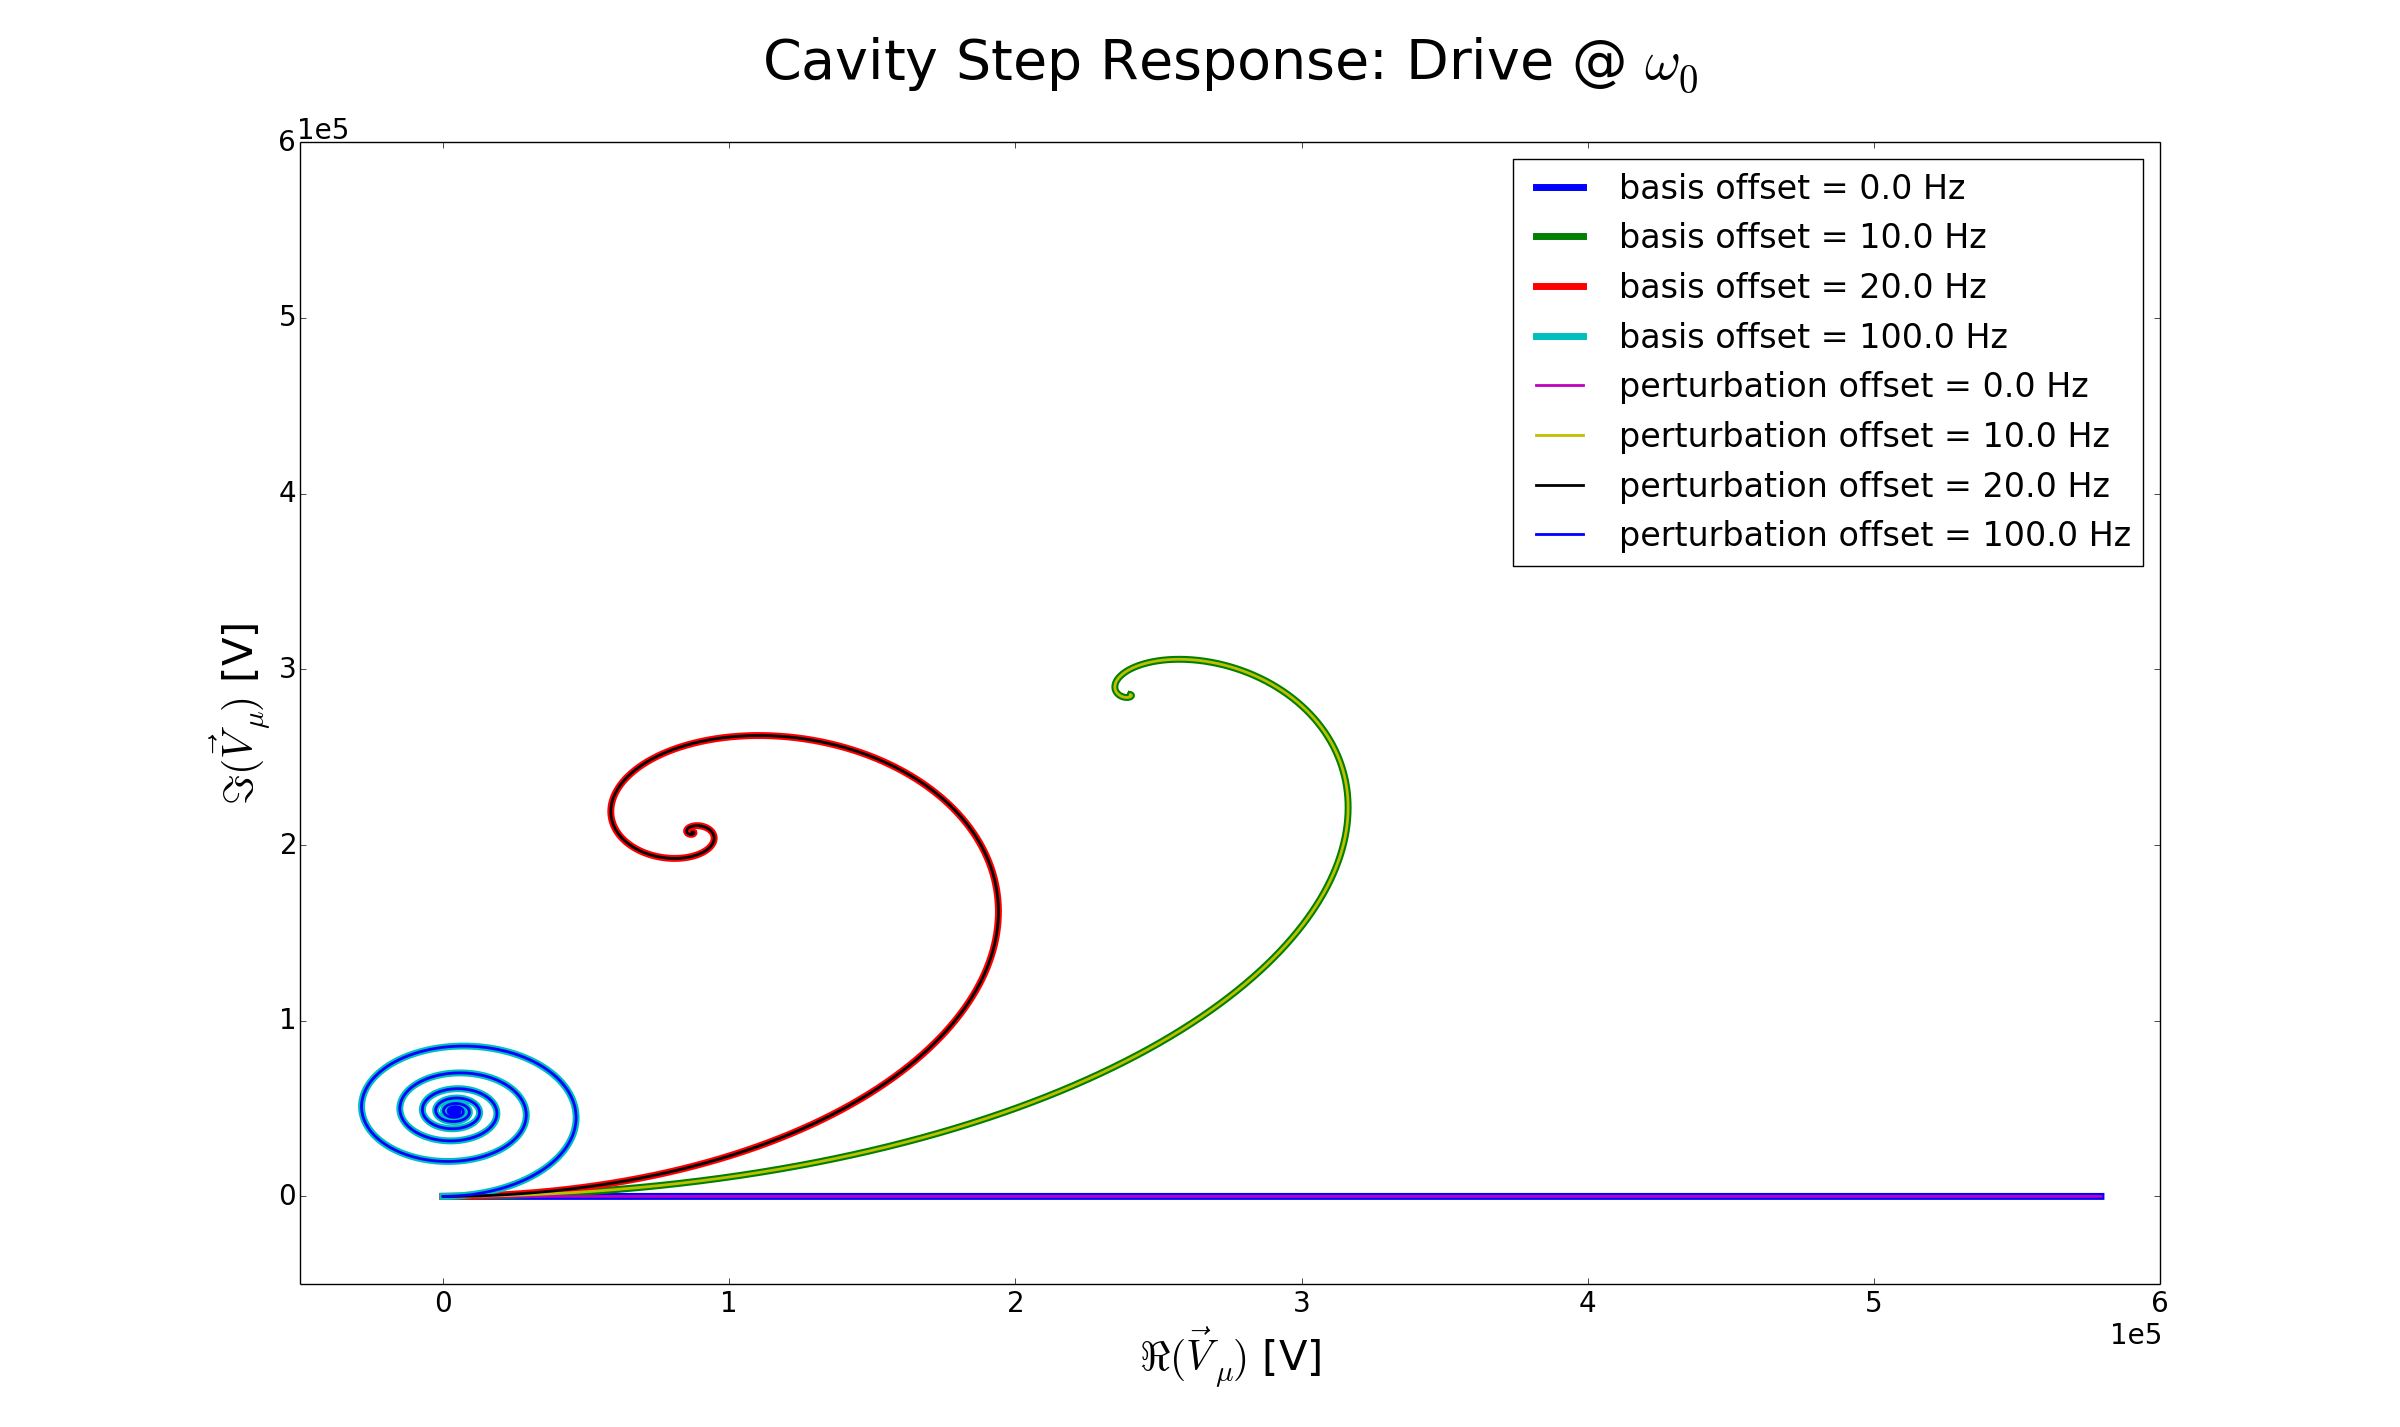
\includegraphics[scale=0.26]{../figures/cavity_test_freqs.png}
\caption{Cavity unit test: Step response RF drive coupling at $\omega_{\rm ref}$ for three different frequency offsets.}
\label{fig:cav_step3}
\end{figure}

At this point we have demonstrated the low-pass filter blocks in Fig.~\ref{fig:RF_cavity_block_diagram} as well as the couplings to the input and output ports. We are now going to demonstrate an important feature (cavity detuning). One can both configure an electrical eigenmode to have a static frequency offset with respect to the RF reference, as well as introducing a time-varying frequency offset due to Lorentz forces or other perturbances.

In Fig~\ref{fig:cav_step3} we introduce a unit amplitude step signal on the RF drive port at the RF reference frequency ($\omega_{\rm ref}$) (instead of at each mode's resonance frequency as in the case of Fig.~\ref{fig:cav_step1}). Each curve is reproduced in two equivalent ways in order to exercise two features of the software: first by sweeping the setting for the so-called basis, or static, offset frequency (the frequency offset between the mode's resonance frequency and the RF reference), and second by sweeping the setting for the frequency shift due to perturbances such as Lorentz forces. All curves correspond to the same mode's accelerating voltage, where only the frequency offset changes, and is plotted in the complex plane to observe the different degrees of ringing as frequency offsets are introduced.

\begin{figure}
\centering
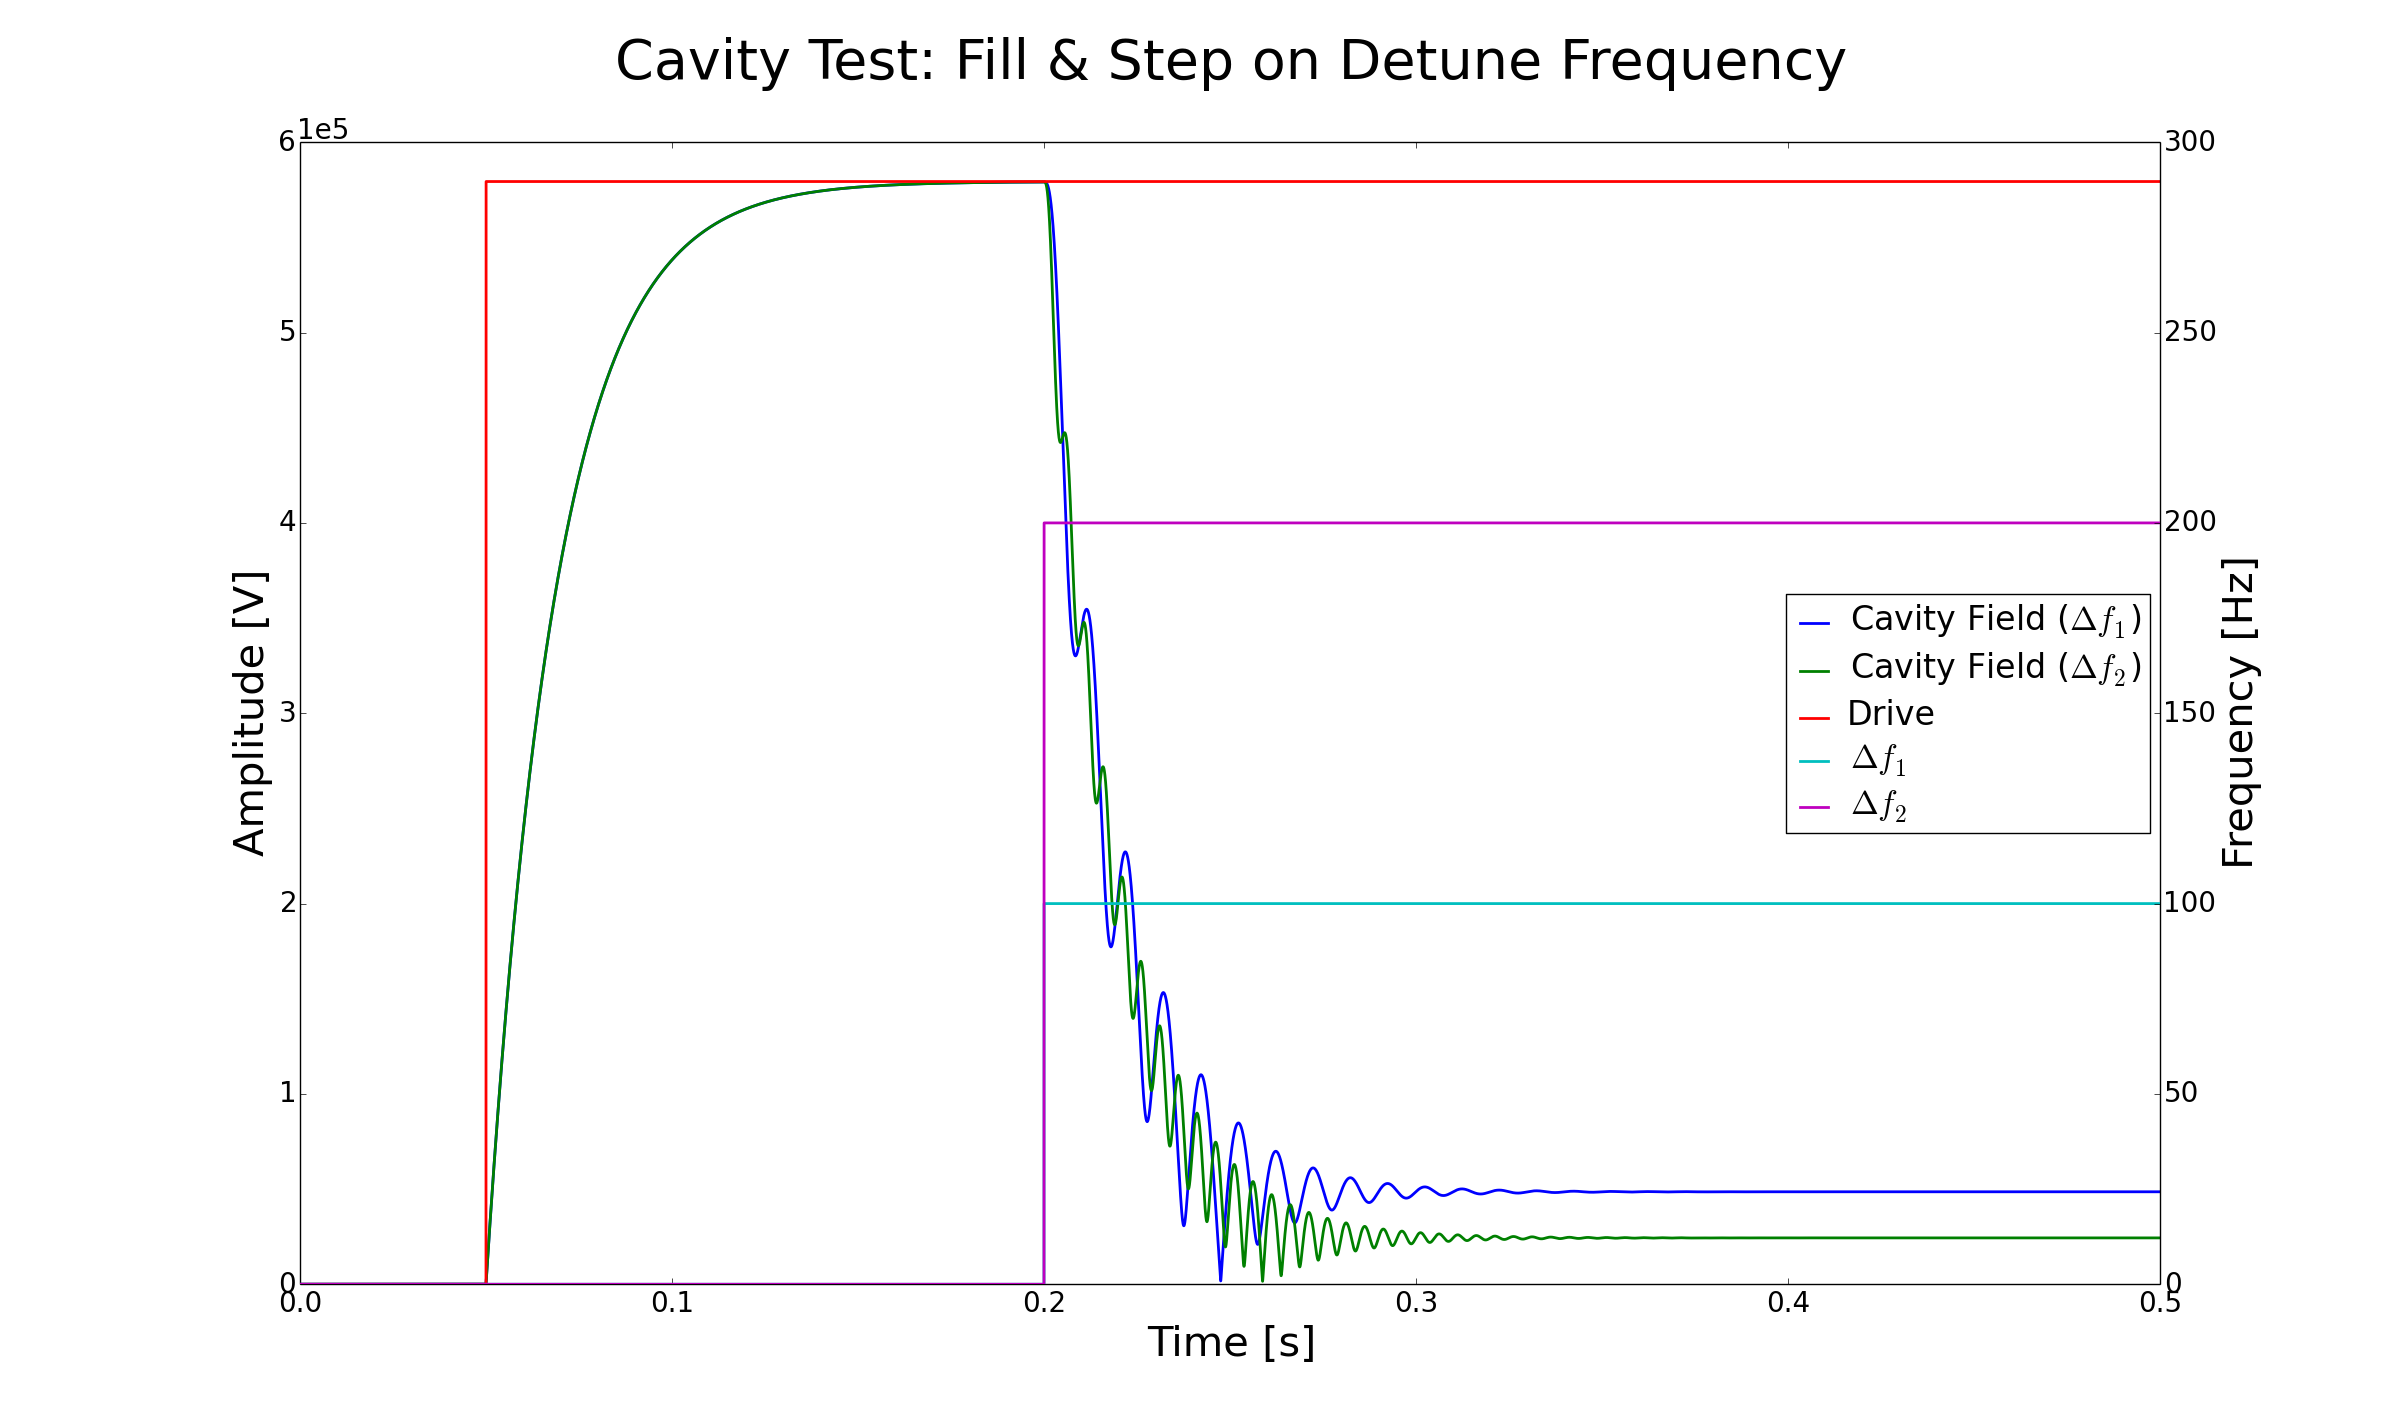
\includegraphics[scale=0.26]{../figures/cavity_test_detune.png}
\caption{Cavity unit test: Step response RF drive coupling at $\omega_{\rm ref}$ and step on the detune frequency.}
\label{fig:cav_step4}
\end{figure}

Fig.~\ref{fig:cav_step4} shows a combination of the previous exercises, where the cavity mode is initially in perfect resonance. A step is applied to the drive signal at the mode's resonance frequency and the cavity field fills up following its time constant (quantified in previous tests). Then, we apply a step to the detune frequency of 10 to 20 times the badwidth of the cavity mode and we observe the cavity decay following its time constant along with ringing induced by the cavity being out of tune. Note that the frequency modulations of the cavity field correspond to the frequency offset applied in each case, and for the case where the step applied is of 100 Hz, the steady-state value is equivalent to the one observed in fig.~\ref{fig:cav_step3} for the same value of freqency offset.

\subsection{FPGA Controller}

Feedback is necessary in order to guarantee the stability of the cavity fields. Latency of the control loop limits the performance of the system and is typically implemented in an FPGA in the form of a Proportional-Integrator (PI) Controller. A flow chart of this controller is shown below, followed by the mathematical expressions. 

%Define block styles
\tikzstyle{block} = [rectangle, draw, node distance = 2.5cm, text width =16em, text centered, rounded corners, minimum height=2em]
\tikzstyle{line} = [draw, -latex']
\tikzstyle{cloud} = [draw, ellipse,  node distance = 3cm, minimum height=2em]
\tikzstyle{circ} = [draw, circle, node distance = 3cm, minimum height = 2em]

\begin{figure}[H]
\centering

\begin{tikzpicture}[node distance = 1cm, auto]
	%Place Nodes
	\node [block, text width = 1cm] (Kp) {$k_{p}$};
	\node [block, below of=Kp, node distance= 1.5cm, text width = 2.2cm] (integrator) {$k_{i} 	 \int_{{0}}^{t} e(\tau)d\tau$};
	\node [circ, left of= Kp, xshift = -1cm](sum){$\Sigma$};
	\node [block, below of=Kp, node distance = 4cm, text width = 2cm](Cavity){Cavity}; 
	\node [block, left of= sum, text width = 1cm] (set point){$\vec{E}_{\rm sp}$}; 
	\node [circ, right of= Kp] (sum1){$\Sigma$};

	\path [line] (sum) -- (-3cm,0) |- (integrator); 
	\path [line] (sum) -- node[near start, anchor = south]{$e(t)$}(Kp);
	\path [line] (integrator) -| (sum1);
	\path [line] (sum1) -- (4cm,0) |- (Cavity); 
	\path [line] (Cavity) -| node[near end]{$-\vec{E}_{\rm probe}$}(sum);
	\path [line] (set point) -- (sum); 
	\path [line] (Kp) -- (sum1);
	\path [line] (sum1) -- node{$\vec{K}_{\rm drive}$}(6cm,0);
	
	
\end{tikzpicture}
\caption{Flow chart of the PI controller}
\end{figure}

Based on different factors, a reference cavity field (set point, $\vec{E}_{\rm sp}$) is chosen as a target. The cavity field is entirely defined by three figures: frequency, amplitude and phase. The feedback control loop described here assumes a fixed frequency for the excitation signal (where cavity detuning can be measured and controlled using other feedback loops) and measures and controls the cavity field amplitude and phase. In the real system, the cavity field is measured using an antenna probe, downconverted, filtered and digitized in the LLRF. As explained earlier, this model works on complex vectors at baseband, where the up and downcoverter circuitry is ommitted. As a result, the model takes discrete values of a sampled cavity field as a complex input and produces a excitation signal to drive the high-power RF source, also a complex vector. In practice, this drive signal is digitized, filtered and up-converted in the LLRF. Here it will be directly connected to the RF amplifier model block as shown in Fig.~\ref{fig:Station_block_diagram}. The error $e(t)$ is defined as the difference between the reference value and the the current measurement of the cavity field $\vec{E}_{\rm probe}$, and the job of the control loop is to minimize this error as much as possible:

\be
e(t) = \vec{E}_{\rm sp} - \vec{E}_{\rm probe}(t)
\ee

\noindent This error is passed onto a proportional and integral controller, with (following text book notation) respective gain constants $k_{p}$ and $k_{i}$. Following the paths, we see that the FPGA drive signal $\vec{K}_{\rm drive}$ is altered according to: 
\be \label{eq: controller}
\vec{K}_{\rm drive} = k_{p} e(t) + k_{i} \int_{\tau_{0}}^{t} e(t) d\tau
\ee

\noindent where $\vec{K}_{\rm drive}$ value is used to drive the high-power RF source feeding the cavity.

\subsubsection{Software implementation}

\begin{figure}
\centering
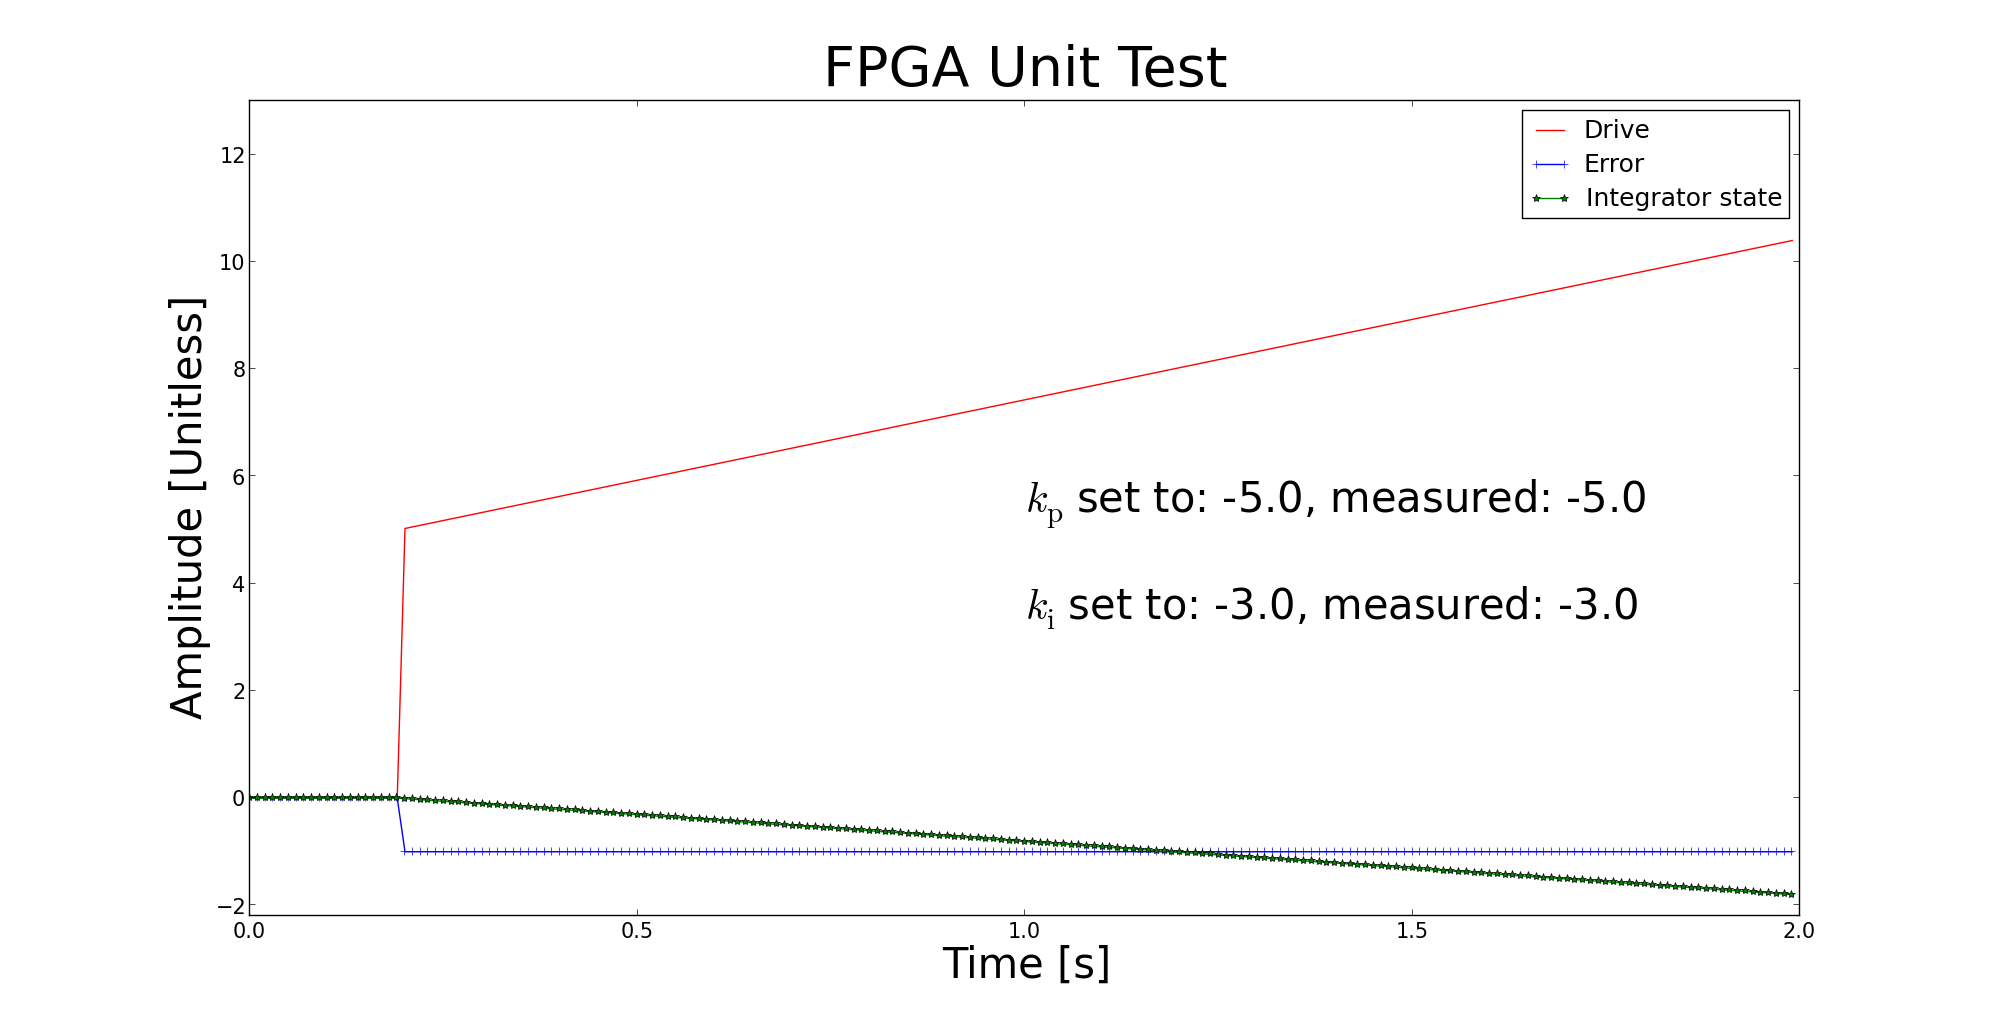
\includegraphics[scale=0.25]{../figures/fpga_unit_test.png}
\caption{FPGA unit test.}
\label{fig:fpga_unit_test}
\end{figure}

In order to implement the PI controller in software, we need to discretize integral term of Equation ~\ref{eq: controller}. This term is shown below. 
\be
k_{i} \int_{\tau_{0}}^{t} e(\tau)d\tau
\ee

There are many ways to evaluate this integral. Most commonly utilized are right-hand, left-hand, and mid-point Riemann sums, Trapezoidal Rule, or Simpson's Rule. In our case, we will simply use a Trapezoidal Rule, which basically comes out to averaging the value of $e(t)$ at the previous and current time step. Considering a very small time step is used, this is a good approximation. Numerically, we have the following for the general case:
\be
\int_{\tau_{0}}^{\tau_{n}} f(\tau) d\tau \approx \Delta t
		    \left[\frac{f(\tau_{0})}{2} + f(\tau_{1}) + f(\tau_{2}) + ...
		      + f(\tau_{n-1}) + \frac{f(\tau_{n})}{2}\right]
\ee

\noindent where the subscript $n$ indicates the time step. To transform to actual time, one merely uses the relationship $\tau_{n} = n\Delta t$. Applied to our problem, we have the following: 

\be
k_{i} \int_{\tau_{0}}^{\tau_{n}} e(\tau)d\tau \approx k_{i}T
	      \left[\frac{e^{0}}{2} + e^{1} + e^{2} + ... 
		+ e^{n-1} + \frac{e^{n}}{2} \right]
\ee

\noindent where again the superscript notation indicates the time step. 

The overall update for $\vec{K}_{\rm drive}$ can then be expressed as:
\be \label{eq: controller_dis}
\vec{K}_{\rm drive}^{n+1} = k_{p} e^{n+1} + k_{i}T \sum_{k=0}^{n}\frac{e^{k+1}+e^k}{2}
\ee

Fig.~\ref{fig:fpga_unit_test} shows the result of a unit tests performed using the software implementation of Eq.~\ref{eq: controller_dis}. The input signal and set-point are initially set to 0 and the FPGA routine is exercised individually, in the absence of a plant or feedback loop. The PI controller is then configured to have certain values of proportional and integral gains ($k_{\rm p}$ and $k_{\rm i}$, as indicated in Fig.~\ref{fig:fpga_unit_test}) and a time-series simulation is run. After 0.1 seconds of simulation, a step is introduced in the set-point (going from 0 to 1) and the drive signal is analyzed. Before any error signal is present in the integrator state, the drive signal is modulated by the set-point by a factor of $k_{\rm p}$. From that point the integrator behavior can be observed, where the slope of the drive signal is given by the integral gain constant $k_{\rm i}$. The measured values of the controller constants (indicated in Fig.~\ref{fig:fpga_unit_test}) are compared with the configuration settings in order to verify the proper behavior of the model.

\subsection{RF Amplifier}

\begin{figure}
\centering
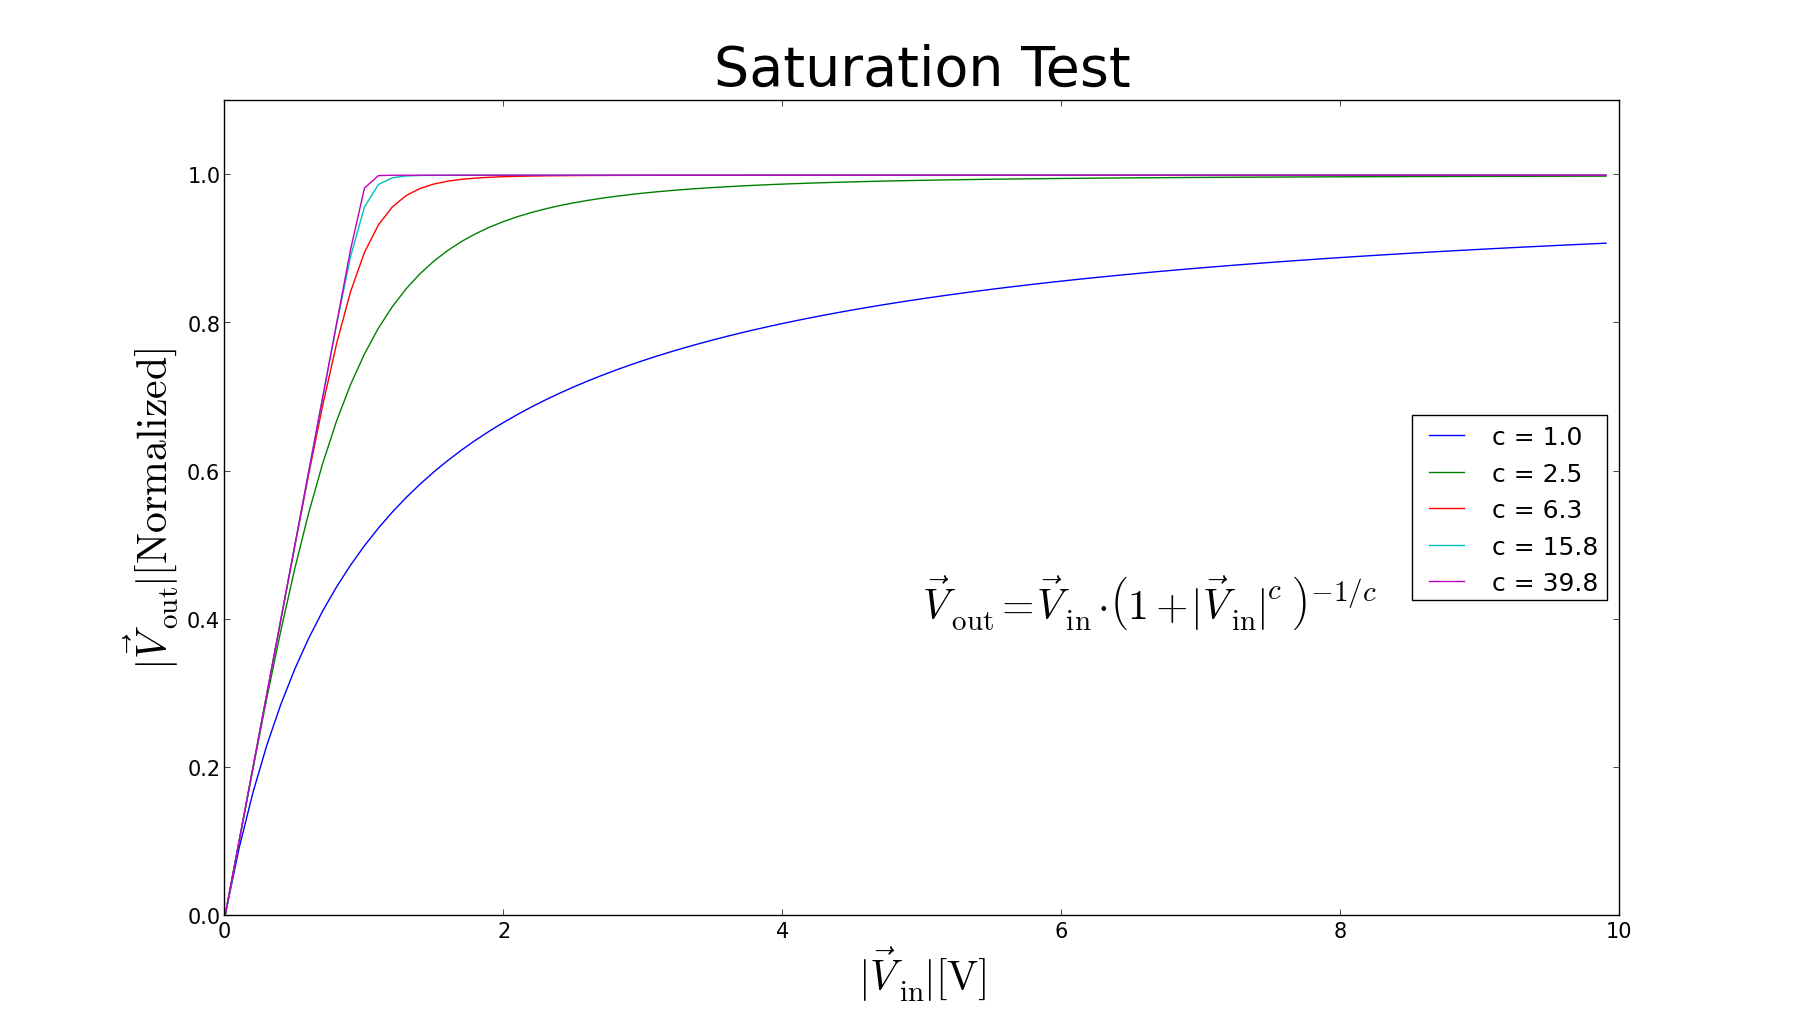
\includegraphics[scale=0.35]{../figures/saturation_test.png}
\caption{RF Amplifier saturation test, where the output is plotted as a function of the input for different values of the harshness parameter c in Equation~\ref{eq:clip}.}
\label{fig:saturation_test}
\end{figure}

For the purposes of including the RF amplifier response in the LLRF simulations we have used two elements: clipping in order to emulate the amplifier saturation curve, combined with a low-pass filter to limit the bandwidth of the amplifier and therefore limit the speed at which the drive signal applied to the cavity can vary. It is useful, in practice, to tweak the configuration of this model in order to match measurements done on the real amplifier in use. Here we propose a clipping equation which has matched RF amplifier saturation curves well in the past. However, if this equation does not match well a particular instance other equations can be chosen.

Amplifier clipping is then described with a harshness parameter c, such that the output signal $\vec V_{\rm out}$, based on its input $\vec V_{\rm in}$ varies according to:

\begin{equation}
  \vec V_{\rm out} = \vec V_{\rm in} \cdot \left(1 + |\vec V_{\rm in}|^c\right)^{-1/c}
  \label{eq:clip}
\end{equation}

The saturated output amplitude from this equation is 1. While some phase shift with drive level is observed in real amplifiers, this effect is not yet included in the model. Fig.~\ref{fig:saturation_test} shows the output of the saturation routine as a function of the input for different values of the harshness parameter c. Note the use of normalized units. In order to obtain units of power, the model is configured to scale these values by the amplifier full-scale input and output values. Also, as described earlier and not shown here is the use of a low-pass filter (typically configured with a cutoff frequency in the MHz range) in order to limit the bandwidth of the amplifier.

\subsection{Phase Shifter}

\begin{figure}
\centering
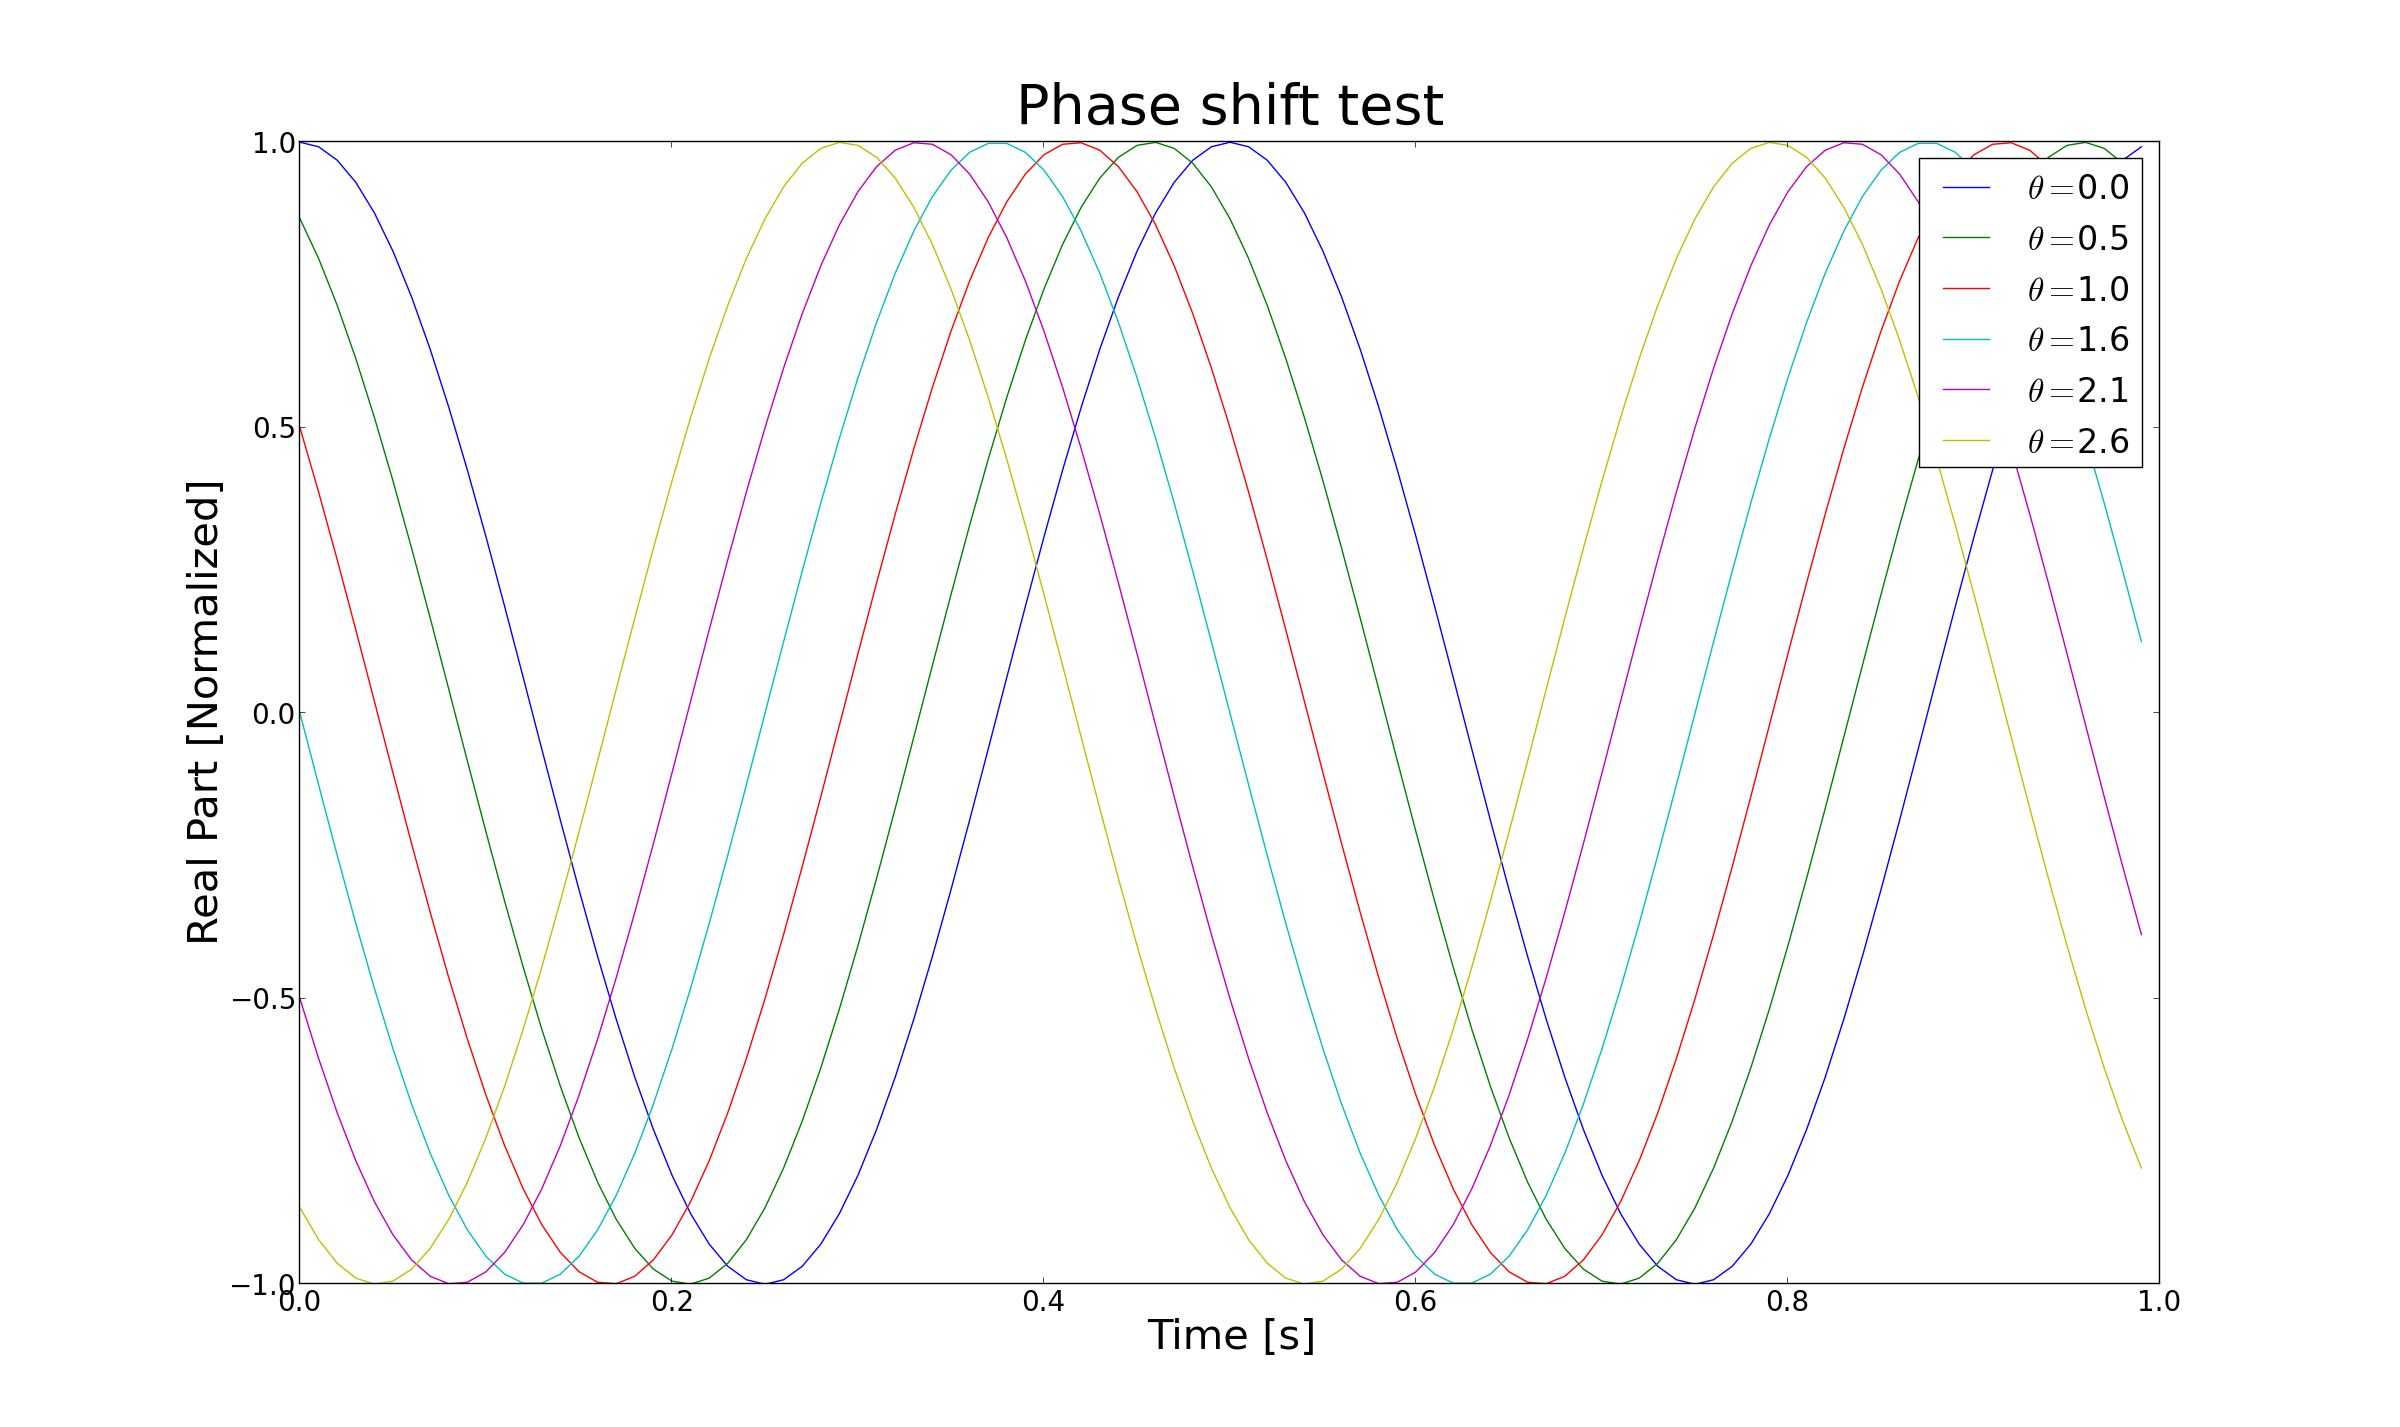
\includegraphics[scale=0.265]{../figures/phase_shift_test.png}
\caption{Phase shift test.}
\label{fig:phase_shfiter_test}
\end{figure}

Phase shifts are encountered at several stages of the model. A phase shifter module (not necessarily explicitly represented in block diagrams) is present in the software implementation and performs a phase shift of an input signal by an angle $\theta$ according to:

\begin{equation}
  \vec V_{\rm out} = \vec V_{\rm in} \cdot e^{j\theta}
\end{equation}

Fig.~\ref{fig:phase_shfiter_test} shows results of a unit tests performed on the phase shifter, where a sample signal is shifted by different angles and the phase differences are measured and compared with the phase angle parameter provided to the phase shifter software routine.

\subsection{LLRF Noise}

LLRF noise is dominated by ADC and preamplifier noise, which typically have broad-band (white) and 1/$f$ components. Here we only consider the broad-band component, as digital LLRF controllers (with {\it in-situ} calibration schemes) are effective at rejecting low frequency noise.

RF systems include several components such as the RF cavity, filters, digitizers, mixers (up and down converters), digital controller, etc. Some of these components are shown the the block diagram in Fig.~\ref{fig:Station_block_diagram}. Since different configurations of the RF system will result in differences in its frequency response, we prefer to express each noise sources in terms of its Power Spectral Density (PSD).

It is useful to express RF analog signal processing and ADC noise in dBc/Hz, where dBc is a logarithmic representation of the ratio between noise and carrier power. In the accelerator case, the carrier represents the nominal cavity signal, in turn something close to the full range of the \hbox{ADC}.  Normalization by the bandwidth gives a true performance number, independent of bandwidth (or equivalently, averaging). As mentioned earlier, we are only considering broad-band noise, so we will use a single noise value expressed in dBc/Hz, being constant over the entire frequency spectrum. This is a figure of merit for the RF measurement channel, which will vary depending on the amplifiers and ADCs used.
%Integrating this noise using the closed-loop frequency response one obtain the noise contribution in dBc (or Volts, or $\rm{V^2}$).

In our simulation models we use pseudo-random number generators to emulate noise sources, and typically express signals in normalized units, where the normalizing factor is the nominal cavity voltage. In the case of LLRF broadband noise, we choose normally distributed pseudo-random generated samples with zero mean and a variance calculated using the LLRF noise specs (in dBc/Hz), the full range of the ADC, and the operating bandwidth.

Let us use as an example the measured noise PSD of the LLRF4 system:
\begin{equation}
  \centering {\rm PSD}_{\rm LLRF} = -135\thinspace{\rm dBc/Hz} = 10^{-13.5} {\rm /Hz}
\end{equation}
The total normalized noise power in a bandwidth $B$ is then
%First we convert from dBc/Hz to dBc integrating over the operating bandwidth (B):
\begin{equation}
  \centering {\rm Noise}_{\rm LLRF} ={\rm PSD}_{\rm LLRF}\cdot B
  \label{eq:PSD_to_noise}
\end{equation}

\noindent If we use $1\thinspace\mu s$ simulation steps ($\Delta t_{sim}$):
\begin{equation}
  \centering B = \frac{1}{2} \cdot \frac{1}{\Delta t_{\rm sim}}=\frac{1}{2} \cdot 1\thinspace {\rm MHz} = 500\thinspace {\rm kHz}
\end{equation}

LLRF systems typically sample the cavity field faster than 1\thinspace MHz. Taking a more realistic sampling rate such as 100\thinspace MS/s ($f_S=100$\thinspace MHz), using $1\thinspace\mu s$ simulation steps would be equivalent to averaging 100\thinspace MHz samples by a factor $n=100$, which leads us to the same result:
\begin{equation}
  \centering B = \frac{1}{2} \cdot f_S \cdot \frac{1}{n} = \frac{1}{2} \cdot 100\thinspace{\rm MHz} \cdot \frac{1}{100} = 500\thinspace{\rm kHz}
\end{equation}

\noindent This means that we can use the simulation step to calculate the bandwidth, independent of the actual sampling rate.  While the choice of the latter has important practical implications, it doesn't affect the noise performance at this abstract level.

Once we know the bandwidth, we can obtain LLRF noise from the PSD using Eq.~\eqref{eq:PSD_to_noise}, which can be expressed as:
\begin{equation}
  \centering {\rm Noise}_{\rm LLRF} = \frac{P_{\rm Noise}}{P_{\rm ADC}}
  \label{eq:dBc_def}
\end{equation}
where $P_{\rm Noise}$ and $P_{\rm ADC}$ can be given in any self-consistent power units, such as $V^2$,
and $P_{\rm ADC}$ refers to the full-scale level of the \hbox{ADC}.
As mentioned earlier, we are interested in expressing the LLRF noise in normalized units, using the nominal cavity voltage as normalizing factor. Considering we design the RF system to provide the ADC with a dynamic range of 1.5 times the nominal cavity voltage as an example, 
%\begin{equation}
%  \centering V_{\rm Noise} (norm.) = \frac{V_{\rm Noise}(V)}{V_{\rm nom}(V)} = \frac{V_{\rm Noise}(V)}{V_{\rm ADC}(V)} \times \frac{V_{\rm ADC}(V)}{V_{\rm nom}(V)}=1.5 \times \sqrt{\frac{P_{\rm Noise}(V^2)}{P_{\rm ADC}(V^2)}}
%  \label{eq:v_noise_norm_def}
%\end{equation}
%where:\\
%$V_{\rm Noise} (norm.) = \mbox{LLRF noise voltage in normalized units,}$
%$V_{\rm nom}(V) = \mbox{Nominal cavity voltage in Volts} \quad \mbox{and} \quad $
%$V_{\rm ADC}(V) = \mbox{Full range of the ADC in Volts}$\\
%Combining Eqs.~\ref{eq:dBc_def} and~\ref{eq:PSD_to_noise}, we find:
%\begin{equation}
%  \centering \frac{P_{\rm Noise}(V^2)}{P_{\rm ADC}(V^2)} = 10^{\frac{Noise_{\rm LLRF}(dBc)}{10}} = 10^{\frac{PSD_{\rm LLRF}(dBc/Hz)}{10}} \times B
%  \label{eq:power_fraction}
%\end{equation}
%and substituting Eq.~\ref{eq:power_fraction} into~\ref{eq:v_noise_norm_def}, we get:
and defining $V_{\rm rms,norm}$ as the root-mean-square noise component added to
normalized cavity voltage, we get:
\begin{equation}
  \centering V_{\rm rms,norm} = 1.5 \cdot \sqrt{{\rm PSD}_{\rm LLRF} \cdot B}
  \label{eq:v_noise_final}
\end{equation}

The above discussion is valid for baseband signals, but LLRF systems digitize the signal
around a carrier frequency, typically using $I/Q$ or near-$I/Q$ sampling of the measured cavity voltages. When sampled at $90^\circ$, the ADC produces a stream of $I, Q, -I, -Q$ samples, which gets repeated over and over again. We therefore get a stream of $I$ and $Q$ samples respectively at half the total rate. Eq.~\eqref{eq:v_noise_final} gives us the noise in one sample as a function of the bandwidth. In order to find the noise of the $I$ and $Q$ samples respectively we need to divide the total bandwidth by a factor of two. Considering $B$ in Eq.~\eqref{eq:v_noise_final} the total bandwidth, we get an identical noise level for both $I$ and $Q$ samples:
\begin{equation}
  I_{\rm rms,norm}= Q_{\rm rms,norm} = \frac{1}{\sqrt{2}}\cdot V_{\rm rms,norm}
  \label{eq:i_q_vs_v_rms}
\end{equation}
This relationship is also valid for near-$I/Q$ sampling after the DSP converts raw ADC samples to digital
$I$ and $Q$.

Now that we have the noise in the $I$ and $Q$ components of the measured cavity voltage, we can calculate the contribution of LLRF noise to both amplitude ($A_{\rm rms}$) and phase ($\Phi_{\rm rms}$) errors.
The general case is a nonlinear transformation that depends on the instantaneous value of the cavity field.
For small amounts of noise around an equilibrium setpoint, which is unity in our normalized treatment,
the results simplify to
\begin{equation}
  A_{\rm rms,norm} = I_{\rm rms,norm}
  \label{eq:a_noise}
\end{equation}
\begin{equation}
  \Phi_{\rm rms,rad} = Q_{\rm rms,norm}
  \label{eq:p_noise}
\end{equation}

Let us now calculate the expected noise levels in both amplitude and phase when using a LLRF4 system (${\rm PSD}_{\rm LLRF}=-135\thinspace$dBc/Hz) and a $1\thinspace\mu s$ simulation step ($B$=500\thinspace kHz). Combining Eqs.~\eqref{eq:v_noise_final} and~\ref{eq:i_q_vs_v_rms}, we get:

\begin{equation}
   I_{\rm rms,norm} = Q_{\rm rms,norm} =  1.5 \cdot \sqrt{\frac{1}{2} \cdot 10^{-13.5} \cdot 500 \times 10^3}= 1.334\times 10^{-4}
\end{equation}
which can then be approximated to amplitude and phase errors using Eqs.~\eqref{eq:a_noise} and~\eqref{eq:p_noise}, where the amplitude error is expressed in normalized units (normalizing factor being the nominal cavity voltage), and the phase error is expressed in radians.

\subsection{Simulation results}


\newpage

\section{Cryomodule}

The cryomodule model shown in Fig.~\ref{fig:Cryomodule_block_diagram} includes a configurable number of RF Station instances (described in detail in Section~\ref{sec:rf_station}), as well as cavity-to-cavity interactions through mechanical couplings. Here we describe the state-space model representing the dynamics of the mechanical resonances (also, as in the case of the electical modes in a cavity, decomposed into eigenmodes) as well as the interactions bewteen these mechanical eignenmodes and the cavity electrical eigenmodes (through Lorentz forces), piezos and tuners.

\begin{figure}
\centering
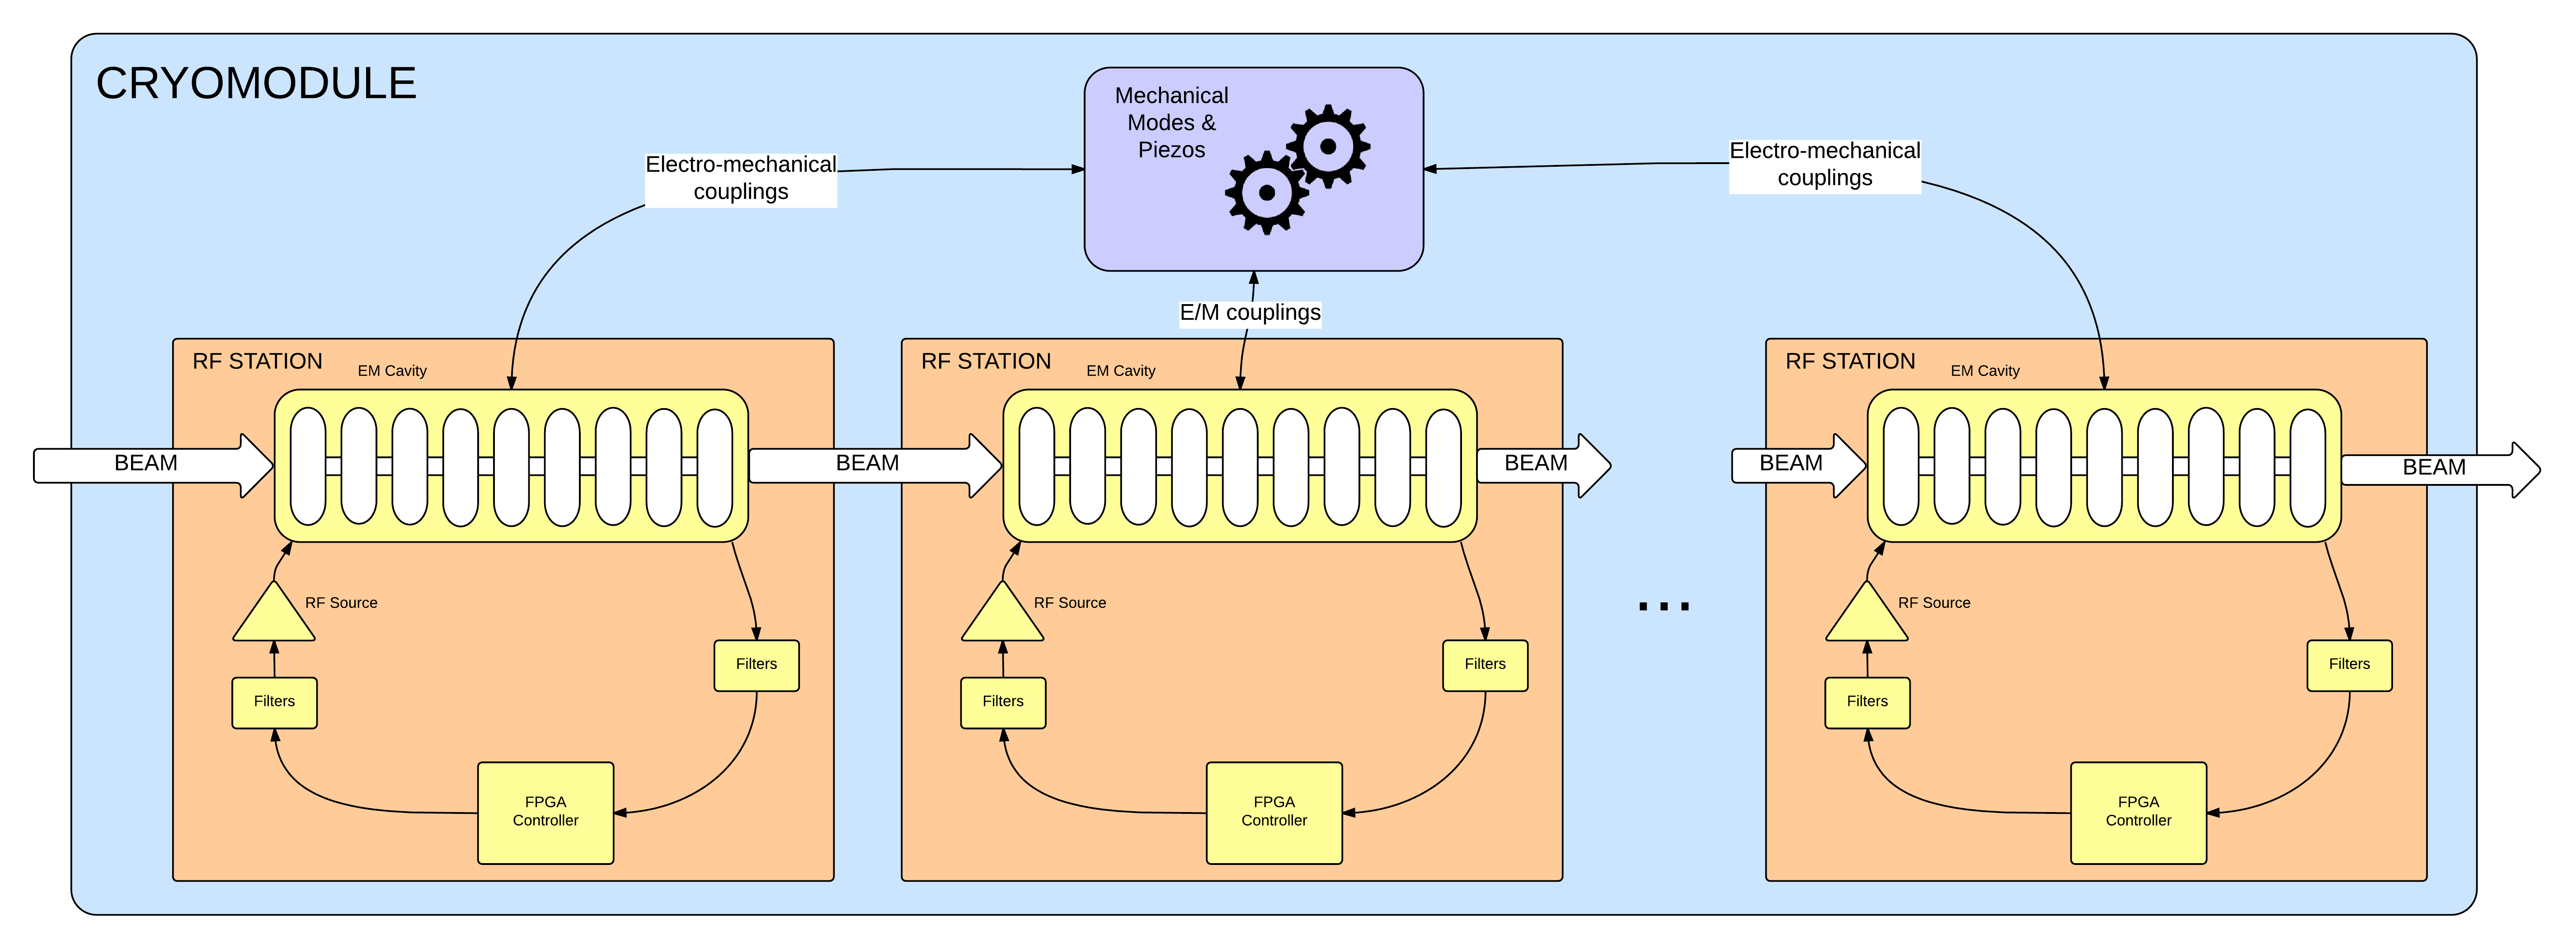
\includegraphics[scale=0.3]{../figures/Cryomodule_block_diagram.png}
\caption{Cryomodule block diagram.}
\label{fig:Cryomodule_block_diagram}
\end{figure}

\subsection{Electro-mechanical interactions}

The presence of an EM field inside the cavity generates forces on the cavity walls, resulting in deformation of the cavity and subsequently in a shift of the cavity resonant frequency~\cite{ref:delayen}, designated in Section~\ref{sec:rf_station} as detune frequency $\omega_{d_\mu}$. Each mode's fields generate a force proportional to $V_\mu^2 = |\vec V_\mu|^2$, and mechanical displacements influence each mode's instantaneous detune frequency.  Construct $\omega_d$ in Section~\ref{sec:rf_station} as a baseline $\omega_{d0}$ from the electrical mode solution ({\it e.g.}, $-2\pi (800\thinspace {\rm kHz})$ for the TTF cavity's $8\pi/9$ mode), plus a perturbation $\omega_{\mu}$ contributed from the mechanical mode deflections. 

Consider the electrical mode index $\mu$ to include not only electrical eigenmodes of one cavity, but modes of all cavities in the mechanical assembly ({\it e.g.}, cryomodule). Also include the dependence on piezoelectric actuator voltages $V_\kappa$. Then if the assembly's mechanical eigenmodes are indexed by $\nu$, mechanical forces $F_\nu$ and displacements $x_\nu$ of those eigenmodes are related to the electrical system by

\begin{figure}
\centering
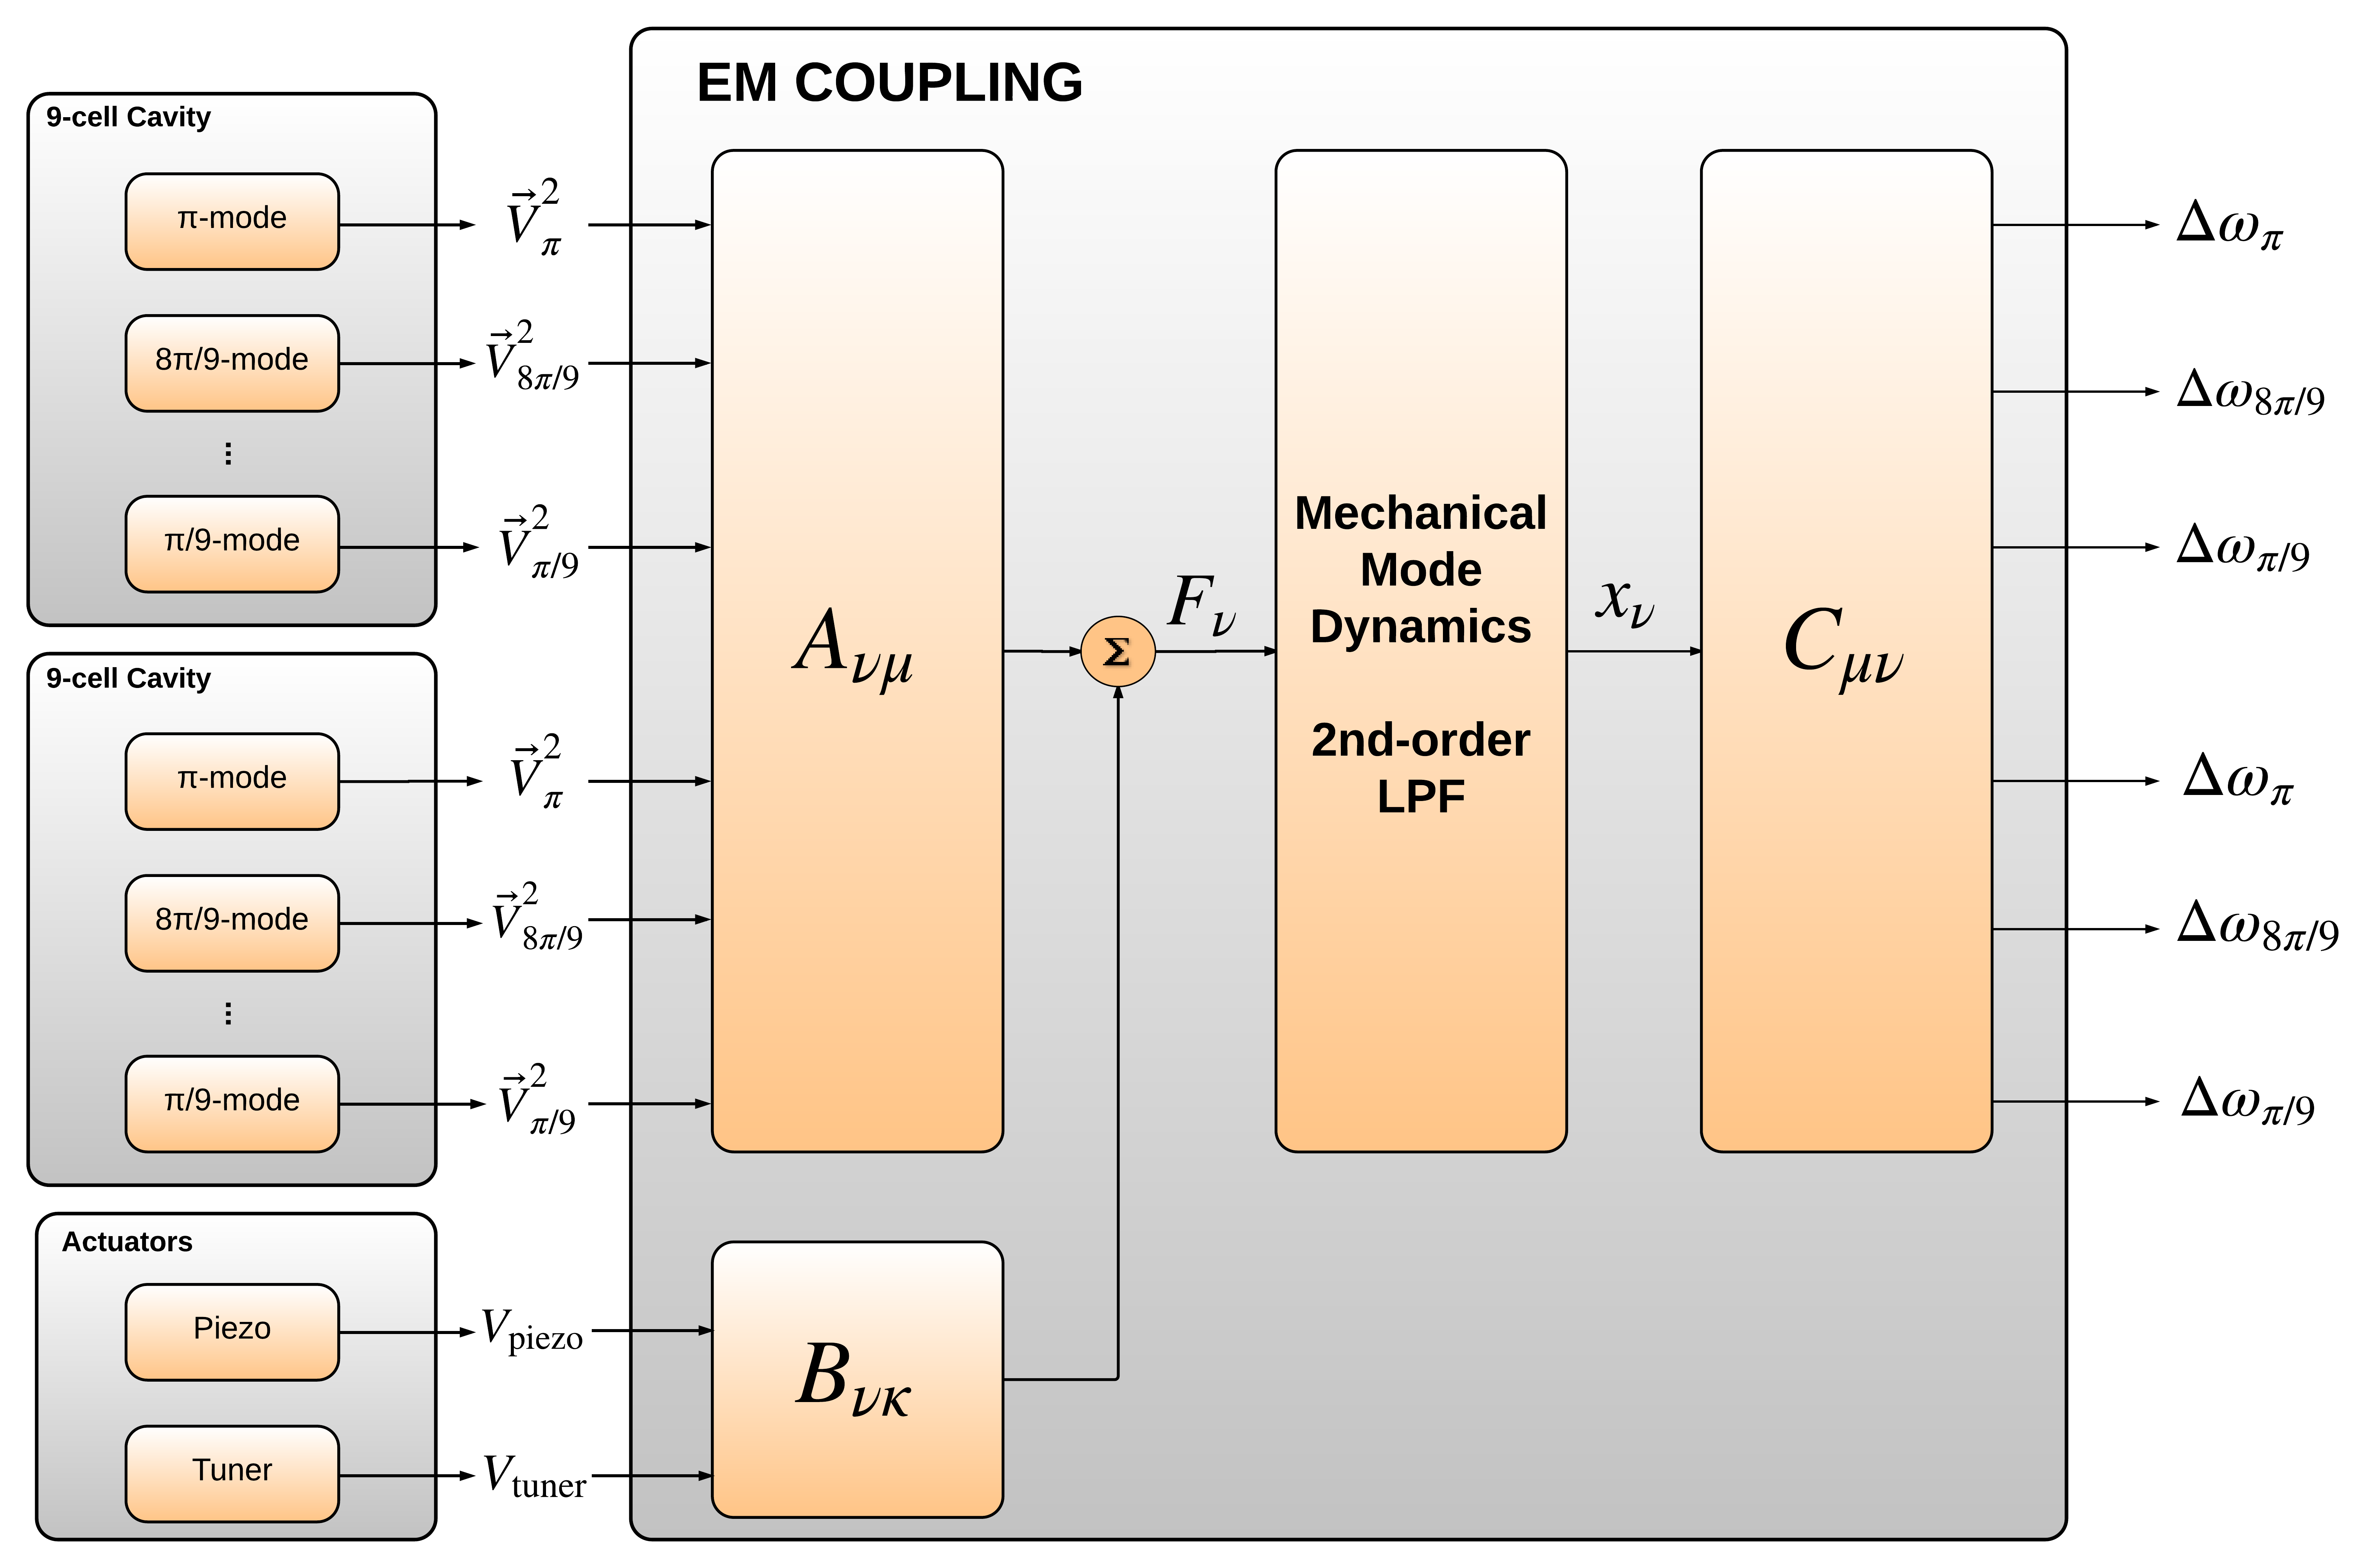
\includegraphics[scale=0.25]{../figures/EM_Coupling_blocks.png}
\caption{Electro-mechanical coupling block diagram.}
\label{fig:EM_couplings}
\end{figure}

\begin{equation}
F_\nu = \sum_\mu A_{\nu\mu} V_\mu^2 + \sum_\kappa B_{\nu\kappa}V_\kappa
\label{eq:F_nu}
\end{equation}

\begin{equation}
\omega_\mu = \sum_\nu C_{\mu\nu} x_\nu~~~,
\label{eq:omega_mu}
\end{equation}

\noindent where $A$, $B$, and $C$ are constant matrices.

These matrix calculations are represented in Fig.~\ref{fig:EM_couplings}. Note that in the same way any electrical eignenmode can be coupled to any mechanical eigenmode, one can configure the matrix to define couplings only present for intra-cavity interactions. In Section~\ref{sec:rf_station} we described in detail how to solve for the accelerating voltages for each electrical mode independently, and the translation between Lorentz forces ($F_\nu$) and mechanical displacements ($x_\nu$) is represented by the state-space model of the mechanical eigenmode described next.

\subsubsection{Mechanical Eignemodes}

Equations~\ref{eq:F_nu} and~\ref{eq:omega_mu} are understood to apply at every time instant; the quantities $V$, $F$, $x$, and $\omega$ all vary with time. The differential equation governing the dynamics of each mechanical eigenmode is that of a textbook second order low-pass filter.  In Laplace form,

\begin{equation}
k_\nu x_\nu = \frac{F_\nu}{ \displaystyle 1 + \frac{1}{Q_\nu}\frac{s}{\omega_\nu} + \left(\frac{s}{\omega_\nu}\right)^2}~~~,
\end{equation}

\noindent where $k_\nu$ is the spring constant. For computational purposes, we want it expressed in terms of the state-space formulation

\begin{equation}
\frac{d}{dt} \begin{pmatrix}
              x_{\nu} \\
              y_{\nu}
             \end{pmatrix}
             = \begin{pmatrix}
                a_{\nu} & -b_{\nu} \\
                b_{\nu} & a_{\nu} \\
               \end{pmatrix}
               \begin{pmatrix}
                x_{\nu}\\
                y_{\nu}
               \end{pmatrix}
               +c_{\nu} \begin{pmatrix}
                  0 \\
                  F_{\nu}
                 \end{pmatrix}
\label{eq: state_space}
\end{equation}

\noindent where a scaled velocity coordinate $y_{\nu}$ has been introduced. Convert the latter equation to Laplace form and solve to get

\begin{equation}
  \begin{pmatrix}
    x_{\nu} \\
    y_{\nu}
  \end{pmatrix}
  = 
  \begin{pmatrix}
    a_{\nu}-s& -b_{\nu} \\
    b_{\nu} & a_{\nu}-s \\
   \end{pmatrix}^{-1}
   \cdot
   \begin{pmatrix}
     0 \\
     F_{\nu}
  \end{pmatrix}
\end{equation}

\noindent Analytically invert that $2\times 2$ matrix, and multiply out to get

\begin{equation}
x_{\nu} = \frac{-b_{\nu}c_{\nu}F_{\nu}}{ (a_{\nu}-s)^2 + b_{\nu}^2}~~~.
\end{equation}

\noindent Equate coefficients with the earlier low-pass filter form, in the case $Q > \frac{1}{2}$, to get

\begin{equation}
a_{\nu}\pm jb_{\nu} = \omega_{\nu}\left( \frac{-1}{2Q_{\nu}} \pm j\sqrt{1-\frac{1}{4Q_{\nu}^2}}\right)
\end{equation}

\begin{equation}
c_{\nu} = -\frac{1}{k_{\nu}}\cdot\frac{a_{\nu}^2+b_{\nu}^2 }{ b_{\nu}} = - \frac{\omega_{\nu}^2}{k_{\nu} b_{\nu}}~~~.
\end{equation}

A deeper understanding of the forces and responses of a single electrical eigenmode $\mu$ of the cavity comes from Slater's perturbation theory.  For an eigenmode solution $\vec H_{\mu}(\vec r)\sin(\omega_{0_{\mu}} t)$, $\vec E_{\mu}(\vec r)\cos(\omega_{0_{\mu}} t)$ to Maxwell's equations in a closed conducting cavity (volume $V$), the stored energy $U_{\mu}$ is given by

\begin{equation} 
U_{\mu} = \int_V \left[ \frac{\mu_0}{4}H_{\mu}^2(\vec r)
                 +  \frac{\varepsilon_0}{4}E_{\mu}^2(\vec r) \right] dv~~~.
\end{equation}

Suppose a mechanical eigenmode $\nu$ involves small deflections $x_{\nu}\cdot \vec\xi(\vec r)$, where $x_{\nu}$ gives the amount of deflection, and the dimensionless quantity $\xi(\vec r)$ represents the mode shape. Both the force on the mode and the response to a deflection $x_{\nu}$ are given in terms of the Slater integral

\begin{equation}
 F_{\mu} = \int_S \left[ \frac{\mu_0    }{ 4}H^2(\vec r)
                 -  \frac{\varepsilon_0}{ 4}E^2(\vec r) \right]
   \vec n(\vec r) \cdot \vec\xi(\vec r) dS ~~~,
\end{equation}

\noindent where $\vec n(\vec r)$ is the normal vector to the cavity surface $S$, and $F_{\mu}$ directly gives the force. Note in particular the subtraction of $E$ and $H$ terms, contrasted with the addition in the energy integral.  Also notice the dot product of the deflection shape with the surface normal.  Then

\begin{equation}
\Delta\omega_{\mu} = -x\omega_{0_{\mu}} \left(\frac{F}{U}\right)_{\mu}
\end{equation}

\noindent and

\begin{equation}
F_{\mu} = \left(\frac{F}{U}\right)_{\mu} \cdot \frac{1}{(R/Q)_{\mu}\omega_{0_{\mu}}}  V_{\mu}^2~~~,
\end{equation}

\noindent where $\left(F/U\right)_{\mu}$ is a property of the electrical eigenmode, independent of amplitude, with units of~\hbox{m$^{-1}$}. Thus 

\begin{equation}
A_{\nu\mu} = \left(\frac{F}{U}\right)_{\mu} \cdot \frac{1}{(R/Q)_{\mu}\omega_{0_{\mu}}}~~~,
\end{equation}

\noindent and 

\begin{equation}
C_{\mu\nu} = -\omega_{0_{\mu}} \left(\frac{F}{U}\right)_{\mu}
\end{equation}

Slater's analysis above lets us express the static Lorentz response as

\begin{equation}
 \left(\frac{\Delta \omega}{ V^2}\right)_{\nu \mu} = \frac{C_{\mu\nu} A_{\nu\mu}}{ k_\nu} = - \left(\frac{F}{U}\right)_{\mu}^2 \cdot \frac{1}{k_\nu (R/Q)_{\mu}}
\end{equation}

\noindent correctly showing that this constant is always negative: the mode's static resonant frequency gets lower as it is filled. Summing over all mechanical modes $\nu$ gives the total DC response, often quoted in units of \hbox{Hz/(MV/m)$^2$}.

Using electrical measurements alone, it's not possible to constrain the scaling of $x_\nu$. It is therefore helpful to rescale $x_\nu$ and $F_\nu$ each by a factor of $\sqrt{k_\nu}$, and eliminate $k_\nu$ from the equations.  Instead of conventional units (m and N) for $x$ and $F$, they now both have units of $\sqrt{\rm Joules}$, so that $x\cdot F$ still represents energy. In this rescaled no-$k$ case,

\begin{equation}
A_{\nu\mu} = \frac{1}{ \omega_{0_{\mu}}} \sqrt{-\frac{1}{ (R/Q)_{\mu}}  \left(\frac{\Delta \omega}{ V^2}\right)_{\nu \mu}}
\end{equation}

\begin{equation}
 C_{\mu\nu} = -\omega_{0_{\mu}} \sqrt{-(R/Q)_{\mu}{ \left(\frac{\Delta \omega}{ V^2}\right)_{\nu \mu}}}\rlap{~~~.}
\end{equation}

It is perhaps an unexpected result that the cross-coupling between cavity modes ({\it e.g.}, excite the $\pi$ mode, measure $\Delta\omega$ for the $8\pi/9$ mode) is quantitatively predicted from measurements of each mode individually, with the exception of the choice of sign of the above radicals.  All that is required is confidence that mechanical modes are correctly identified and non-degenerate.

\subsubsection{Software implementation}

\begin{figure}
\centering
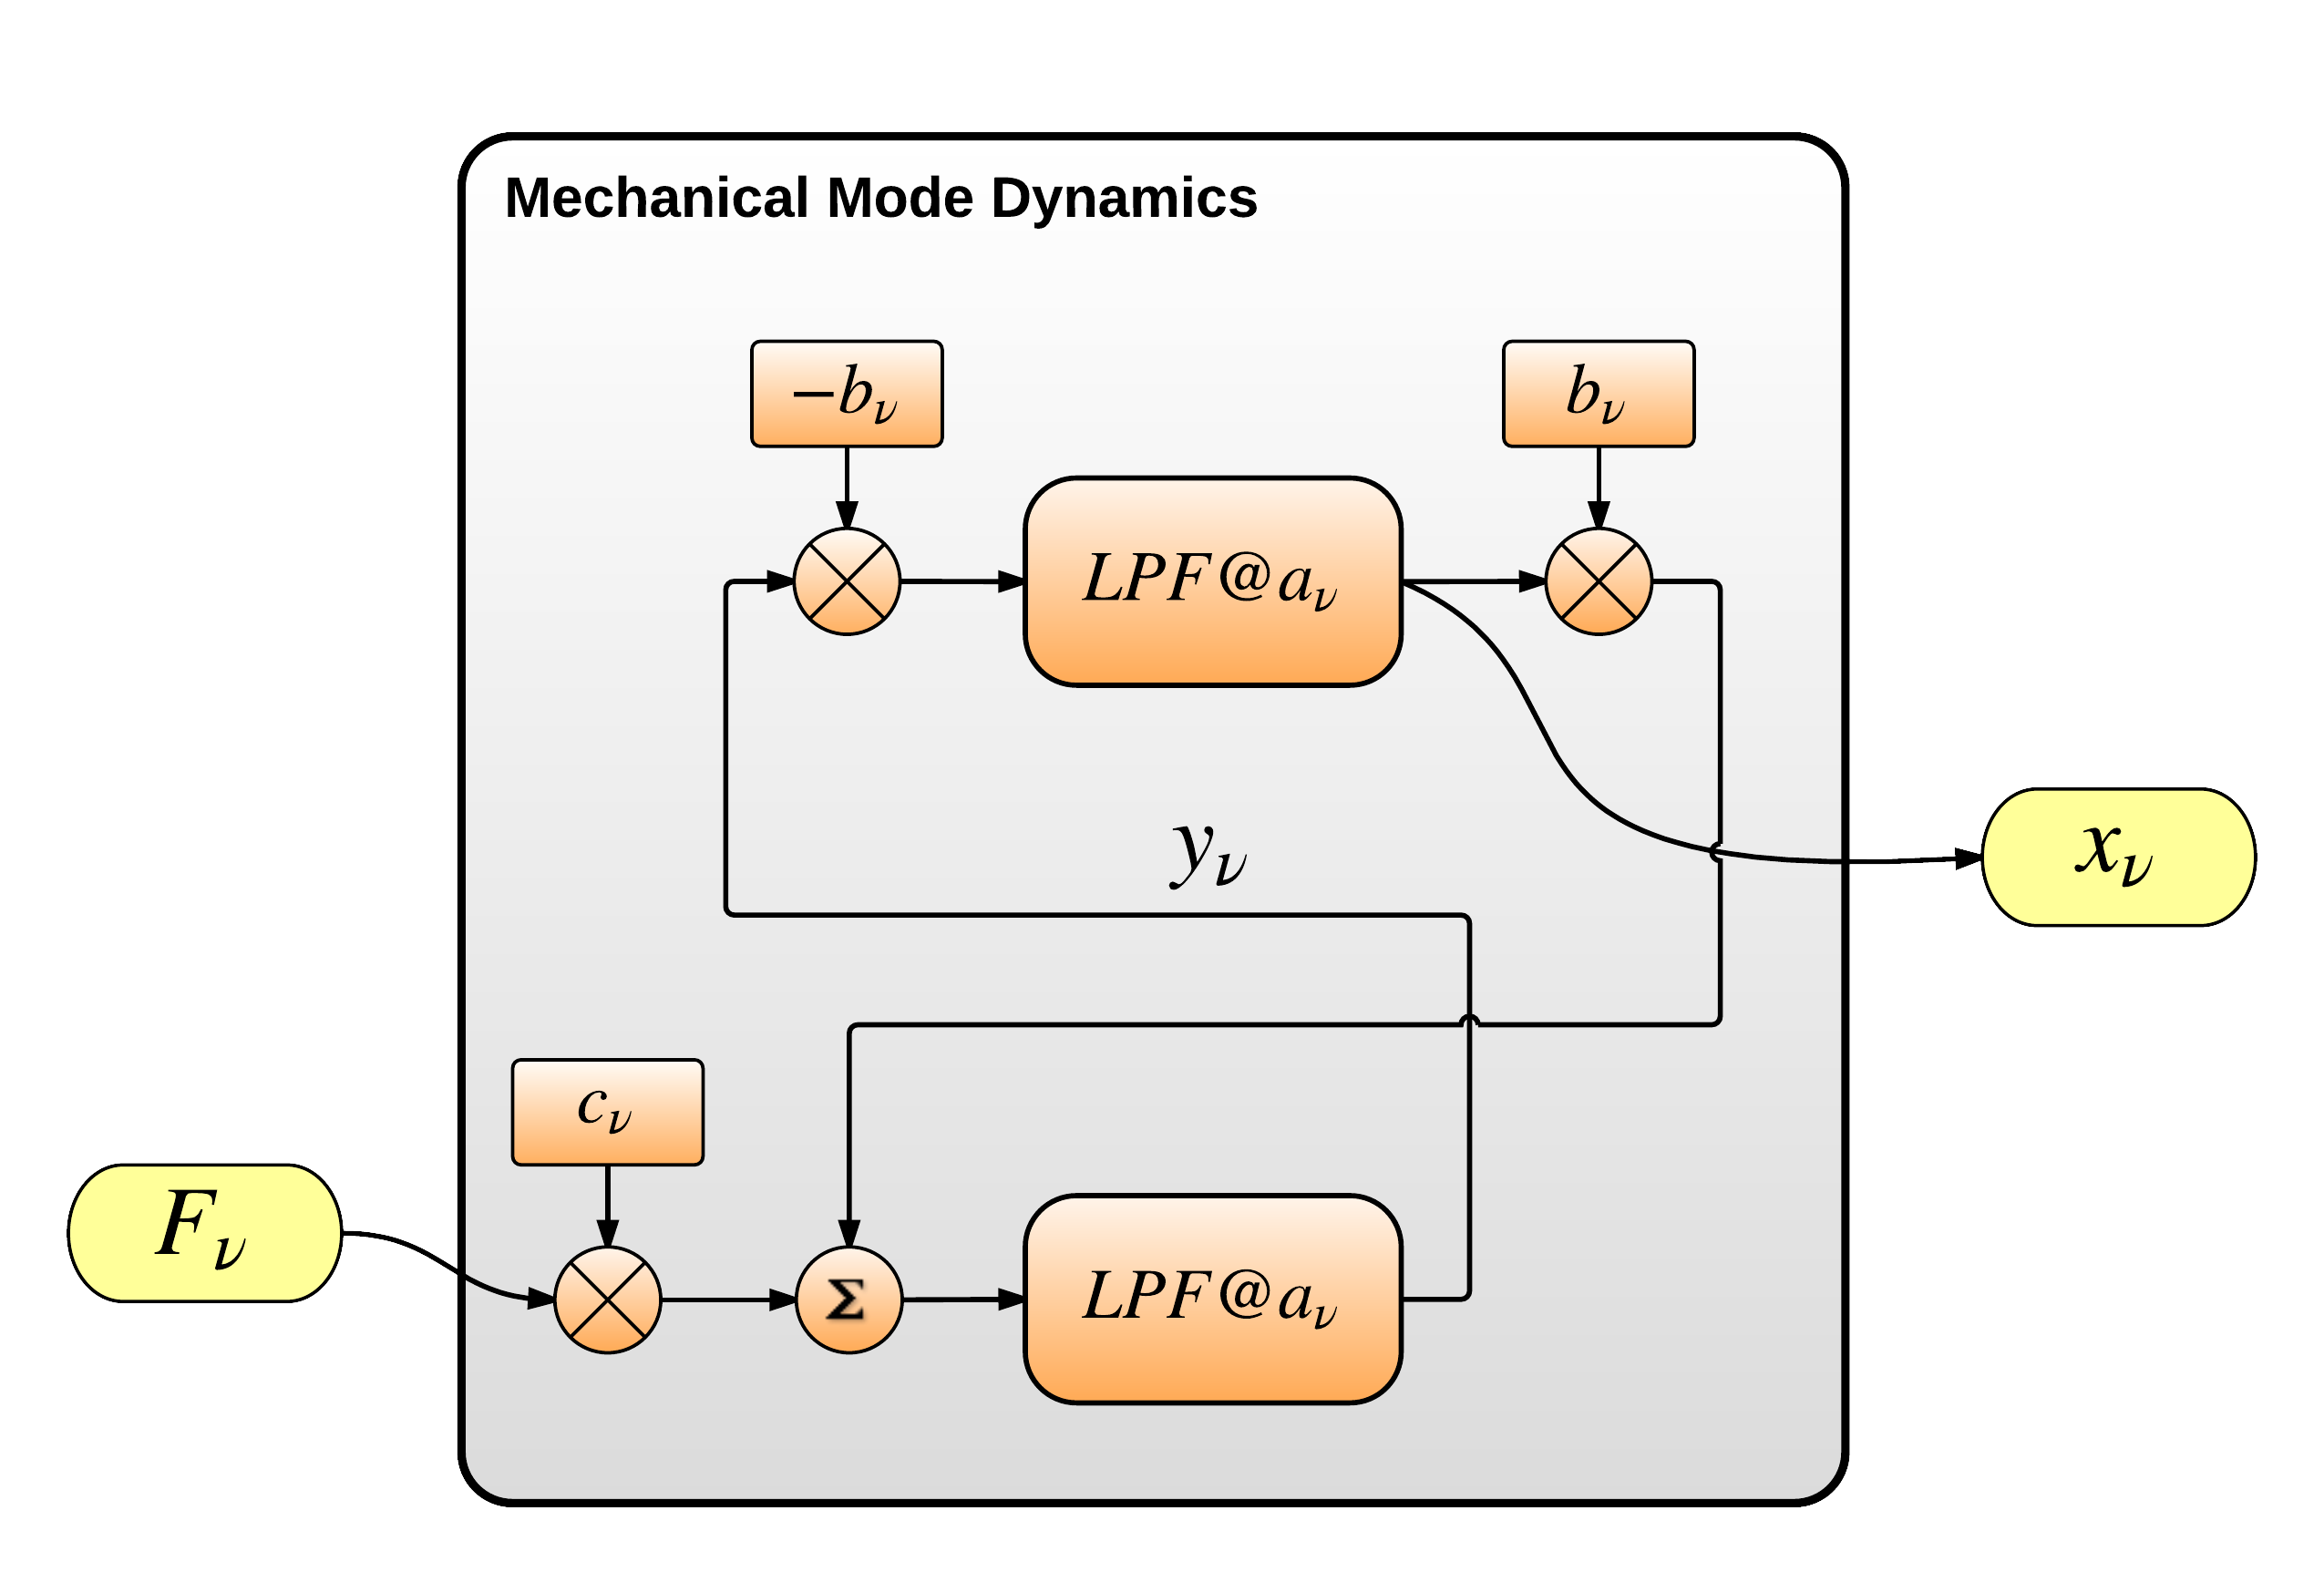
\includegraphics[scale=0.55]{../figures/mech_state_space_blocks.png}
\caption{Mechanical mode dynamics block diagram, second order low-pass filter.}
\label{fig:mech_state_space}
\end{figure}

The matrix calculations shown in Fig.~\ref{fig:EM_couplings} are applied every time step following Equations~\ref{eq:F_nu} and~\ref{eq:omega_mu}. The box labeled ``Mechanical Mode Dynamics, 2nd-order LPF'' takes Lorentz forces for each mechanical eigenmode as an input ($F_{\nu}$) and produces a mechanical displacement ($x_{\nu}$). This corresponds to Equation~\ref{eq: state_space}, the the state-space formulation of the 2nd-order low-pass filter. Expanding that equation in matrix form, two expressions appear:

\begin{equation}
  \frac{dx_{\nu}}{dt} = a_{\nu}x_{\nu} - b_{\nu}y_{\nu}~~~.
  \label{eq:dx/dt}
\end{equation}

\noindent and

\begin{equation}
  \frac{dy_{\nu}}{dt} = b_{\nu}x_{\nu} + a_{\nu}y_{\nu} + c_{\nu}F_{\nu}
  \label{eq:dy/dt}
\end{equation}

\noindent where: 

\be
a_{\nu} =  \frac{-\omega_{\nu}}{2Q_{\nu}} 
\ee
\be
b_{\nu} = \omega_{\nu} \sqrt{1 - \frac{1}{4Q_{\nu}^{2}}} 
\ee
\be
c_{\nu} = -\frac{\omega_{\nu}}{k_{\nu}b_{\nu}}
\ee

These displacements influence each electrical mode's instantaneous eigenmode frequency $\omega_{\mu}$ as follows:

\be
\omega_\mu = \sum_\nu C_{\mu\nu} x_\nu
\label{eq:sum_w_mu}
\ee

\noindent where $C$ is the coupling matrix from mechanics to EM.

The combination of Equations~\ref{eq:dx/dt} and~\ref{eq:dy/dt} is illustrated in Fig.~\ref{fig:mech_state_space}, where the 2nd-oder low-pass filter is implemented as two cascading 1st-order low-pass filters. The blocks labeled ``$LPF@a_{\nu}$'' are instances of the same block used in the cavity state-space model. As in the case of the electrical eigenmodes, equations~\ref{eq:dx/dt} and~\ref{eq:dy/dt} are in the form of a 1st-order differential equation, for which the ODE integration is derived in Appendix~\ref{App:ODE_integration}, where Equations~\ref{eq:dx/dt} and~\ref{eq:dy/dt} can be written as Equation~\ref{eq:exp_diff2}. In this case, the variable matching is as follows:

\begin{equation}
 \vec V_{\rm out} = x_{\nu} \mbox{ , } p = a_{\nu} \mbox{ and, } \vec V_{\rm in} = -b_{\nu}y_{\nu}~~~,
\end{equation}

\noindent and

\begin{equation}
 \vec V_{\rm out} = y_{\nu} \mbox{ , } p = a_{\nu} \mbox{ and, } \vec V_{\rm in} = b_{\nu}x_{\nu} + c_{\nu}F_{\nu}
\end{equation}

\noindent respectively.

At this point we have covered the mechanical state-space model physics and software implementation, as well as the electro-mechanical interactions. We have then all the elements needed in order to perform time-series simulation runs and some results are presented next.

\subsection{Simulation results}

\newpage

\section{Linac Section}

A Linac section is composed of a series of cryomodules potentially followed by a bunch compressor. It is at this level that the longitudinal beam dynamics phase-state model is computed along with the state-space models we have described so far for each one of the Linac components.

\begin{figure}
\centering
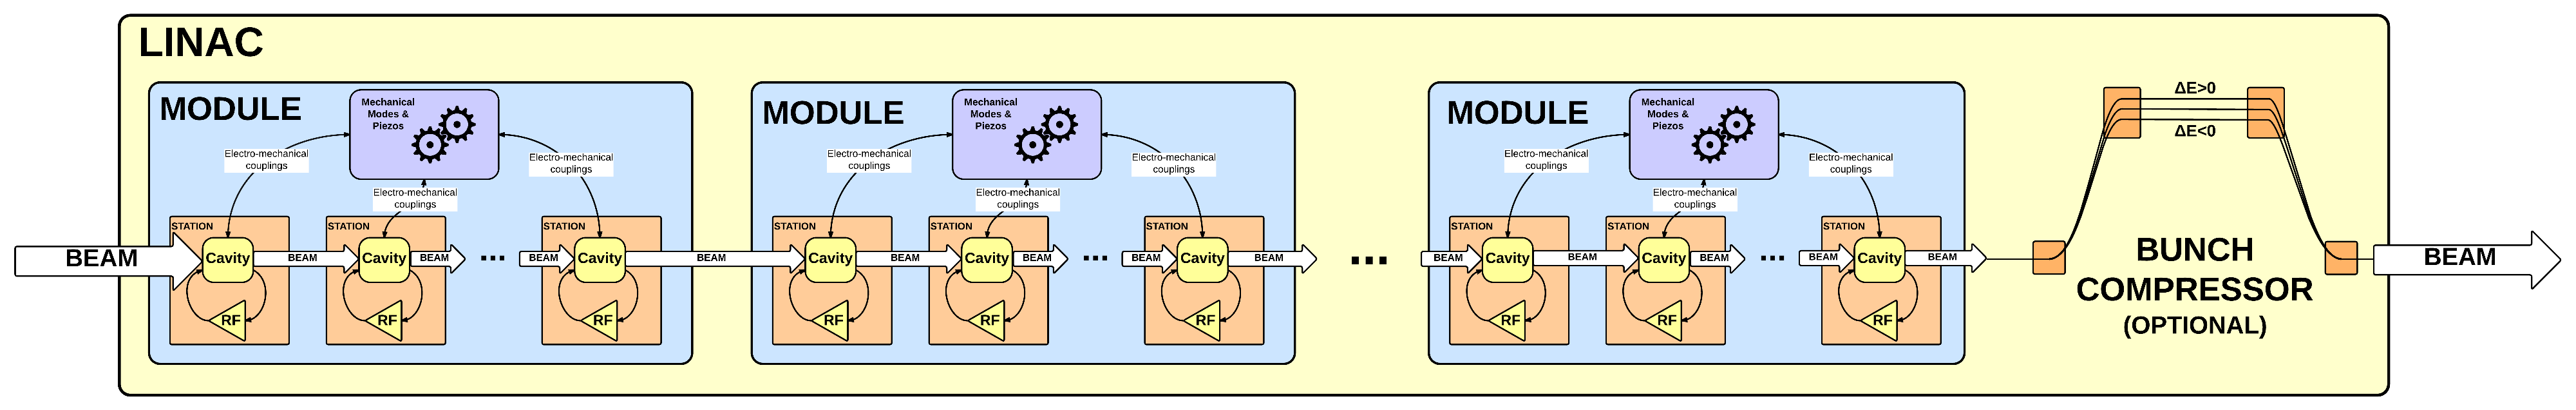
\includegraphics[scale=0.45]{../figures/Linac_block_diagram.png}
\caption{Linac block diagram.}
\label{fig:Linac_block_diagram}
\end{figure}

\subsection{Longitudinal Dynamics Phase-Space model}

\section{Accelerator Model}

\subsection{Noise sources}
\subsection{Beam-based feedback model}
\subsection{State-Space \& Phase-Space Integration}


\section{Conclusions}

\newpage

\begin{appendix}

\section{Appendix}

\subsection{ODE Integration of single-pole low-pass filter}
\label{App:ODE_integration}

\begin{figure}
\centering
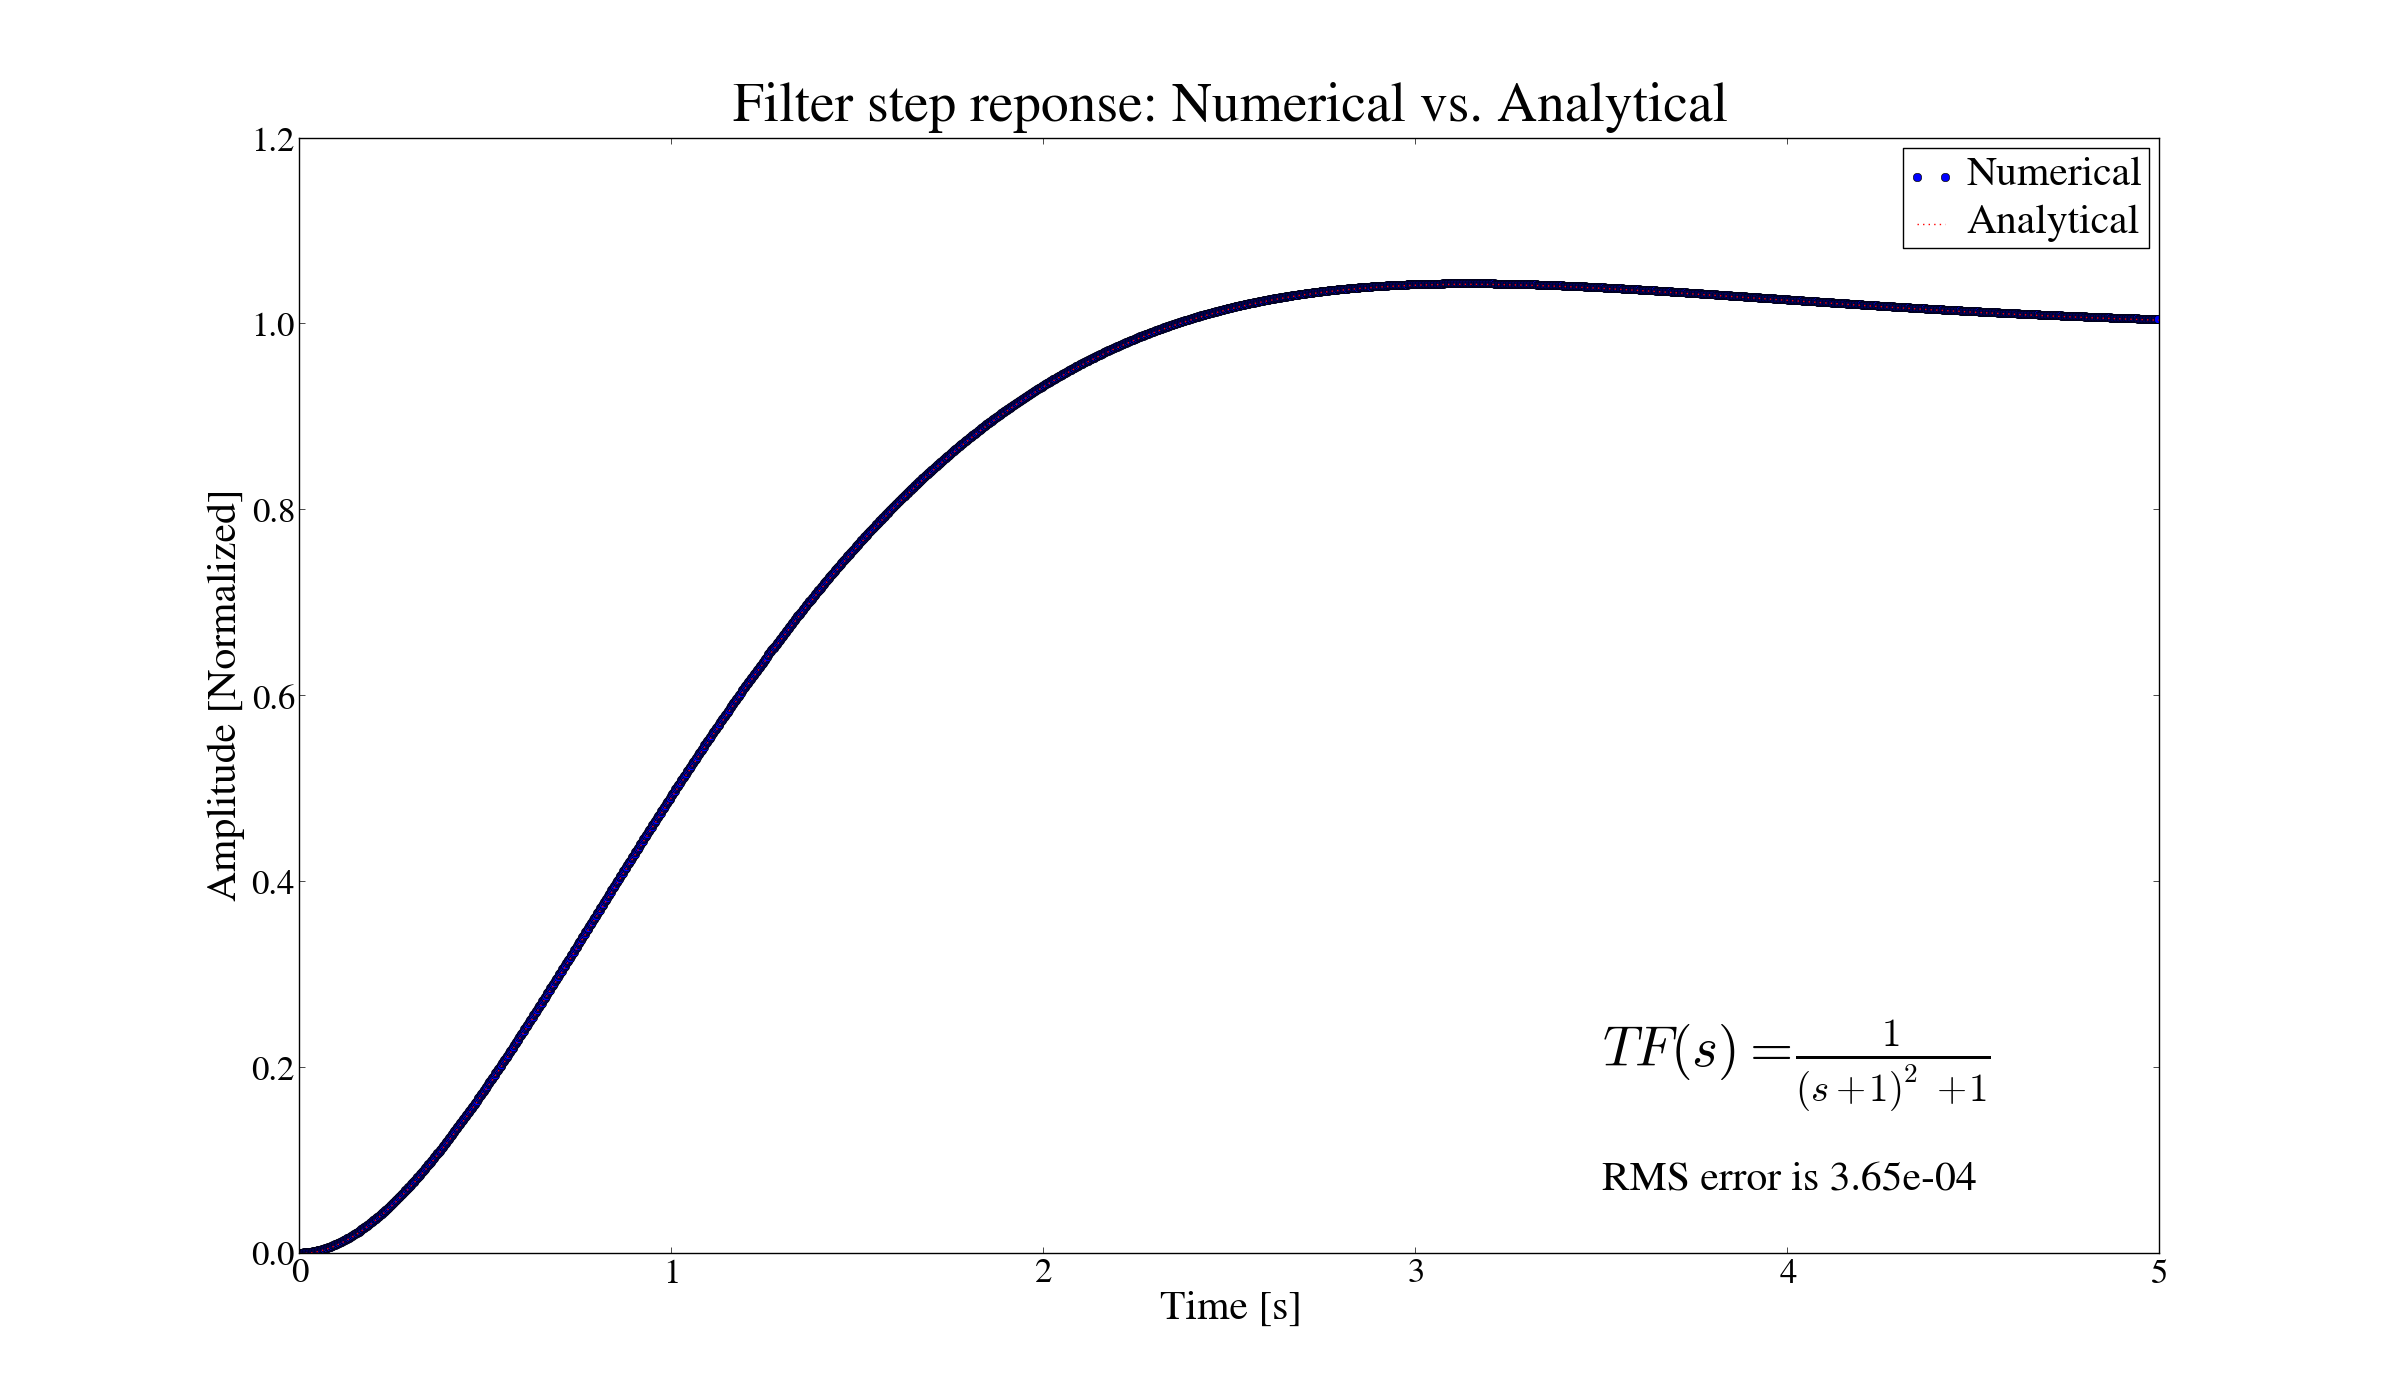
\includegraphics[scale=0.265]{../figures/filter_step_response.png}
\caption{Comparison between numerical and analytical filter step response.}
\label{fig:filter_step_response}
\end{figure}

% \begin{figure}
% \centering
% 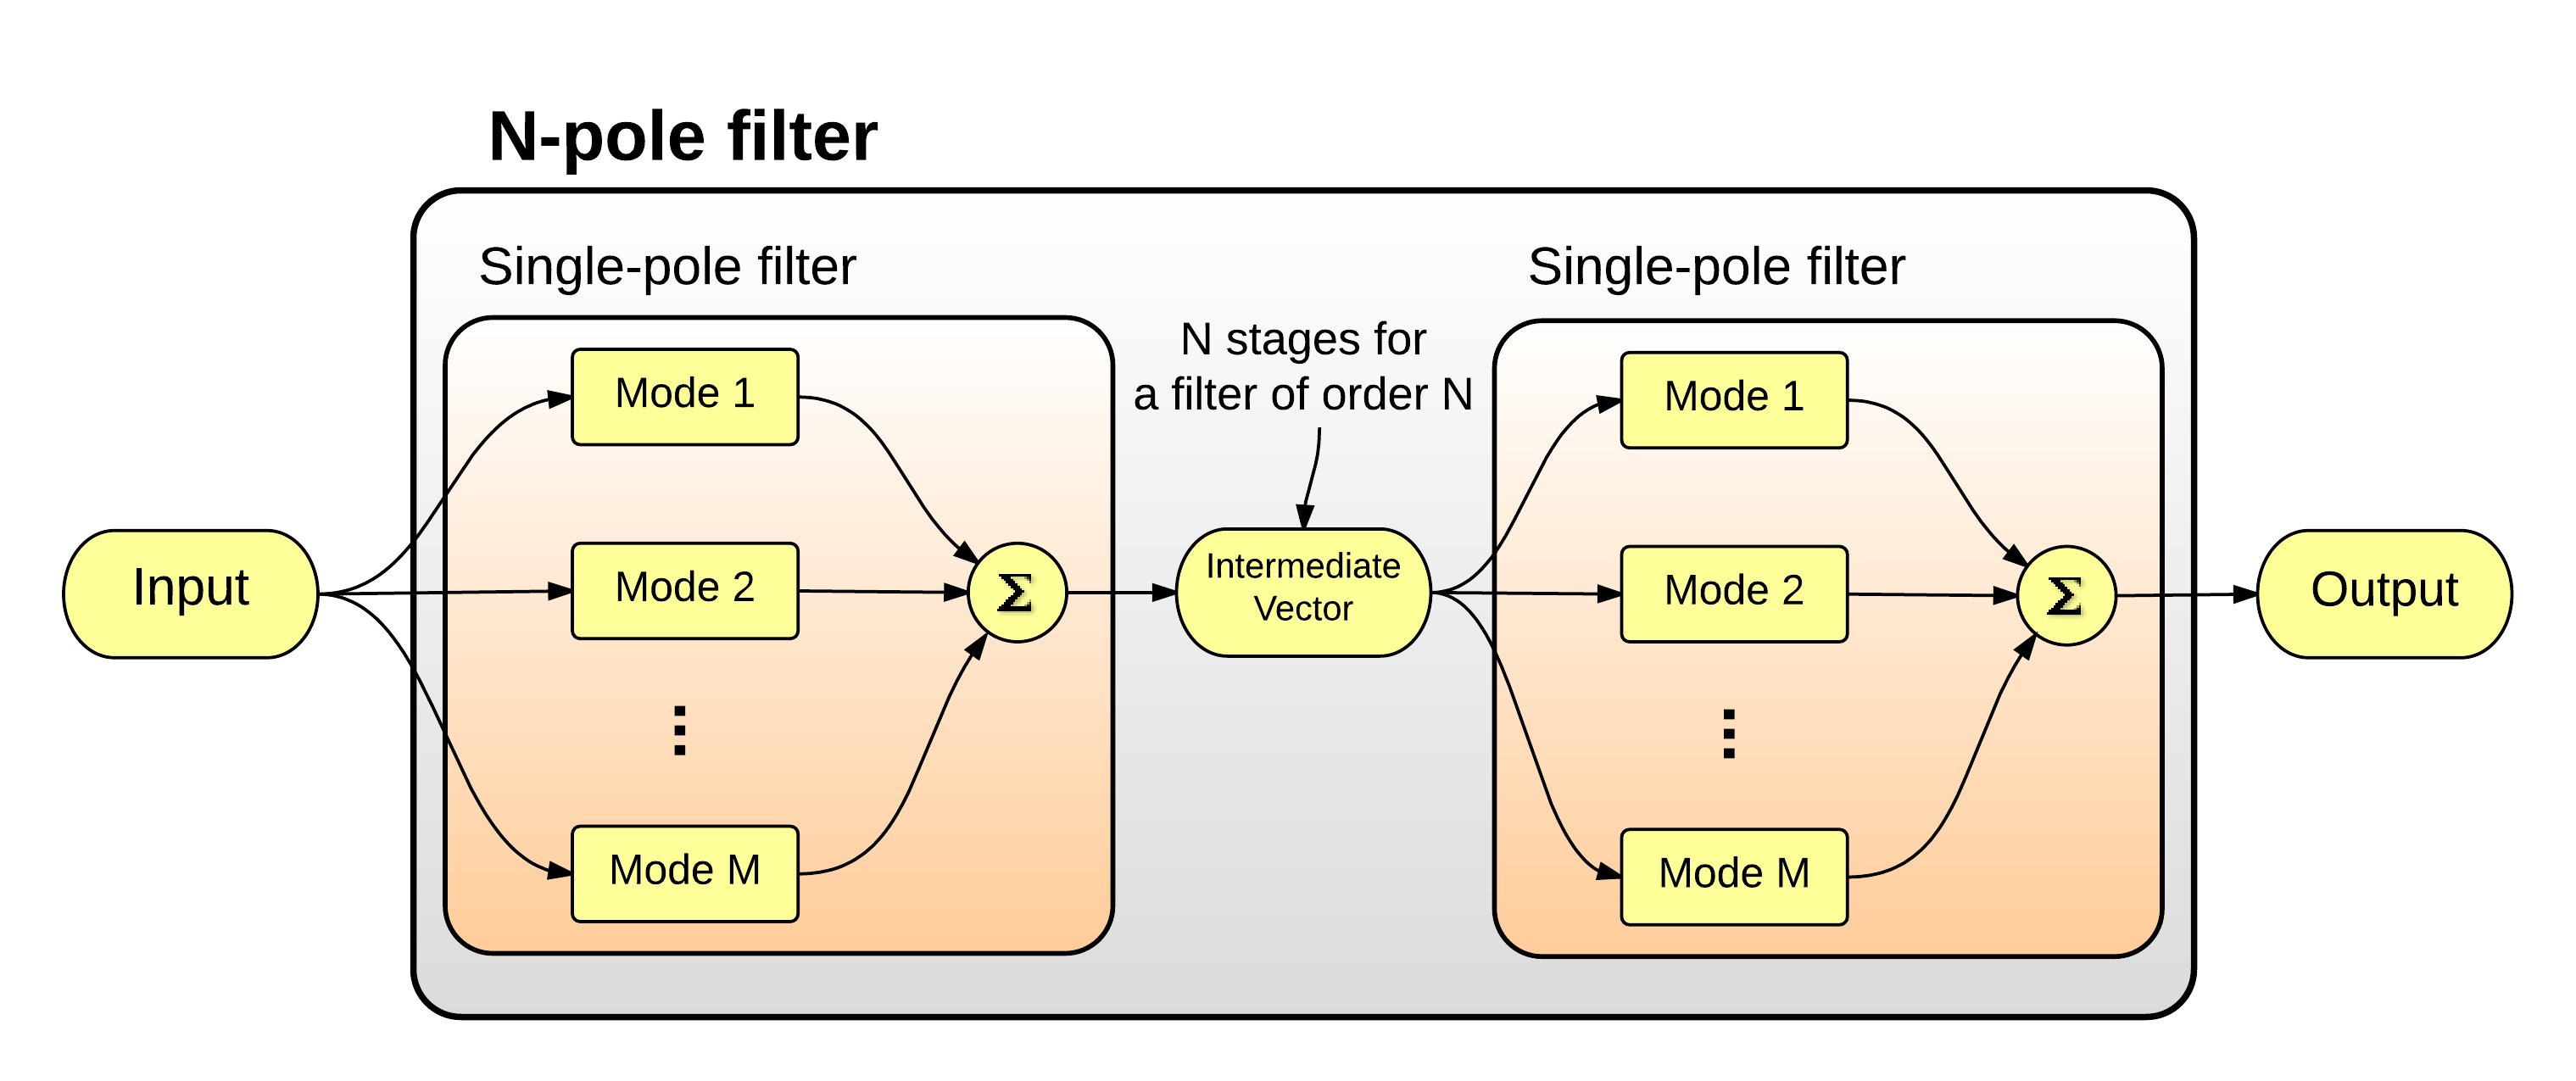
\includegraphics[scale=0.6]{../figures/filter_block_diagram.png}
% \caption{Generalized N-pole filter block diagram.}
% \label{fig:filter_block_diagram}
% \end{figure}

Start with the first order differential equation for a single-pole low pass filter. Its transfer function is expressed in Laplace form as

\begin{equation}
 TF(s)=\frac{\vec V_{\rm out}(s)}{\vec V_{\rm in}(s)} = \frac{1}{s-p}
\end{equation}

\noindent where $\vec V_{\rm in}$ and $\vec V_{\rm out}$ are the input and output signals, and $p$ is the pole location. Make the differentiation explicit, and rearrange to get a form consistent with state-variable numerical ODE integration,

\begin{equation}
 \frac{d\vec V_{\rm out}(t)}{dt} = \vec V_{\rm in}(t) + p\cdot \vec V_{\rm out}(t)
\label{eq:exp_diff}
\end{equation}

The simplest expression for a 'next' value at step $n$ in a discrete time \emph{ansatz} is

\begin{equation}
 \vec V_{\rm out}^n = \left( 1 + \Delta t \cdot p\right) \vec V_{\rm out}^{n-1} + \Delta t \cdot V_{\rm in}^n
\end{equation}

\noindent To improve convergence properties in the case where $\Delta t \cdot p$ is not tiny, approximate the trajectory of $\vec V_{\rm in}$ and $\vec V_{\rm out}$ as linear within a single time step. Specifically, assume that $\vec V_{\rm out}$ changes from $\vec V_{\rm out}^{n-1}$ to $\vec V_{\rm out}^n$, and $\vec V_{\rm in}$ changes from $\vec V_{\rm in}^{n-1}$ to $\vec V_{\rm in}^n$.

Using what is essentially the Trapezoidal Formula~\cite{ref:trapezoid}, our rendition of the discrete time approximation to the above differential equation becomes

\begin{equation} \label{eq:approx}
 	\vec V_{\rm out}^n=a \cdot \vec V_{\rm out}^{n-1}+\frac{1}{2}\cdot b \cdot (\vec V_{\rm in}^{n-1}+\vec V_{\rm in}^n)
\end{equation}

\begin{eqnarray}
	\nonumber \mbox{where} \quad a=\frac{1+ \frac{1}{2} \Delta t \cdot p}{1-\frac{1}{2}\Delta t \cdot p}, \quad \mbox{and} \quad b=\frac{\Delta t}{1-\frac{1}{2}\Delta t \cdot p}
\end{eqnarray}

\noindent $\Delta t$ is the simulation step duration, and $p$ is the pole location (a complex number). Cavity detuning is represented by a slight pole shifting into the imaginary direction.

In order to preserve scaling and have unity gain at DC, Eq.~\ref{eq:exp_diff} needs to be scaled by a factor of p, such that

\begin{equation}
 \frac{d\vec V_{\rm out}(t)}{dt} = p \cdot \vec V_{\rm in}(t) + p\cdot \vec V_{\rm out}(t)
\label{eq:exp_diff2}
\end{equation}

\noindent which is equivalent to scaling $\vec V_{\rm out}^n$ by a factor of $|p|$ in the software implementation.

This process is coded in C, and tested using a two-pole ow pass Butterworth filter. Given the transfer function $1/((s+1)^2+1)$, which has poles at (-1+1j) and (-1-1j), 
the step response is $1 - e^{-t} (\sin x + \cos x)$, for $t > 0$. This analytically known response is plotted in Fig.~\ref{fig:filter_step_response} along with the response obtained using the numerical model.


\end{appendix}

\newpage

\begin{thebibliography}{19}   % Use for  1-9  references

\bibitem{ref:model-paper}
M. Mellado Munoz, L. Doolittle, P. Emma, G. Huang, A. Ratti, C. Serrano, J. M. Byrd, ``A Dynamic feedback model for high repetition rate LINAC-Driver FELs,''
IPAC'12, New Orleans, LA, May 2012.

\bibitem{ref:litrack} 
P. Emma, K. Bane, L. Freitag, ``LiTrack : A Fast longitudinal phase space tracking code with graphical user interface'', PAC'05,  Knoxville, TN, May 2005.

\bibitem{ref:superfish}
Poisson Superfish Software, \url{http://laacg.lanl.gov/laacg/services/download_sf.phtml}

\bibitem{ref:montgomery}
C. G. Montgomery, R. H. Dicke. E. M Purcell, ``Principles of Microwave Circuits'', MIT Radiation Lab Series V8, 1947.

\bibitem{ref:svea}
Slowly varying envelope approximation (SVEA), \url{http://en.wikipedia.org/wiki/Slowly_varying_envelope_approximation}.

\bibitem{ref:schilcher}
T. Schilcher, ``Vector Sum Control of Pulsed Accelerating Fields in Lorentz Force Detuned Superconducting Cavities'', Hamburg 1998.

\bibitem{ref:cell_modes}
L. R. Doolittle, ``Understanding 5-cell mode structures'', JLab tech note CEBAF-TN-0120, May 1989.

\bibitem{ref:delayen}
J. R. Delayen, ``Ponderomotive Instabilities and Microphonics -- A Tutorial'', SRF'05, Ithaca, NY, July 2005.

\bibitem{ref:trapezoid}
Abramowitz and Stegun, ``Handbook of Mathematical Functions'', Formula 25.5.3, 1964.


\end{thebibliography}

\end{document}